\chapter{Methodology}\label{ch:methodology}
% This section will describe the data used (in terms of it's properties such as wavelengths z-steps, timelapse lengths (if consistent), the source of the cell cultures and the make of the microscope used) and why the data was collected in this way (confocal for 3D resolution, treatments applied for mitophagy). Section for methodology employed for auto thresholding

With Chapter \ref{chp:Background} providing background context for the 
\section{Dataset acquisition process and preparation}\label{sec:Dataset_making}
%this section describes properties surrounding the data acquisition, structures labelled (organelles), the fluorophores used, the treatments applied and concisely why, the reason for confocal microscopy (3D resolution and reduced out-of-focus fluorescence), and imaging parameters such as z-step size etc. such that someone could hypothetically reproduce this.
The image data set that was acquired for this research project is composed of microscopy images that can be used in mitophagy analysis. This is due to the primary intended application of this automated binarization system being in the high-throughput pre-processing of microscopy images in mitophagy research.
\subsection{Sample preparation prior to imaging}
%This subsection must discuss what cell types were used, the treatments applied, the organelles stained and the reasons (briefly)
\subsubsection*{Cell culturing}
MEF and GT1-7 cell lines were used and were maintained in Dulbecco's Modified Eagle Medium (DMEM) (ThermoFisher, \#41965062) supplemented with 10\% fetal bovine serum (FBS) (Sigma-Aldrich, \#F0679) and 1\% Penstrep (Sigma-Aldrich, \#P4333) and were kept in a humidified incubator at 37$^{\circ}$C and 5\% CO2. Cells were subcultured using trypsin (Sigma-Aldrich, \#T4049) to detach cells from flasks. Afterwards, DMEM was added to the cells at a 2:1 ratio and cells were collected into 15 mL Falcon tubes (Bio-Smart Scientific, \#50050). Cells were centrifuged at 1500 rpm at room temperature for 3 minutes (Centrifuge, Eppendorf, \#5804R). Media was discarded and cells were resuspended in fresh DMEM. Cells were seeded to T25 flasks (Bio-Smart Scientific, \#70025) 8-chamber dished (ThermoFisher, \#Z734853).
\subsubsection*{Treatments applied}
All treatment interventions were made up using 1x phosphate-buffered saline. The treatments applied were memantine hydrochloride (Sigma-Aldrich, \#PHR1886), carbonyl cyanide m-chlorophenylhydrazone (CCCP) (Sigma-Aldrich, \#857815), and bafilomycin A1 (Baf) (Sigma-Aldich, \#B1793). Only the GT1-7 cells were treated with Memantine hydrochloride which was done by incubating the treatment with the cells at working concentrations of either 50 $\mu$M (LM) or 100 $\mu$M (HM), low and high concentration dosage respectively, for 48 hours prior to any imaging and while refreshing any memantine-treated media every 24 hours. The CCCP treatment was incubated 6 hours prior to imaging at 10 $\mu$M causing mitochondrial depolarization with the goal of increasing the frequency of mitophagy events to observe them. The Baf treatment was incubated with the cells 4 hours prior to imaging at 400 nM to inhibit the completion of mitophagy by preventing the fusion of lysosomes and autophagosomes (described in Section \ref{subsec:lysosome}) resulting in damaged mitochondria to remain contained in autophagosomes. Different combinations of these treatments formed treatment groups, with no treatments forming a control group, so that observations from the analysis could be better correlated with the appropriate treatments.
\textcolor{red}{I feel that this, due to being basically copied from Sholto, should reference the same paper in case it is flagged for plagiarism}
\subsection{Image acquisition via microscopy}
%Briefly discuss the resolution used, the fluorophores in terms of cross-talk, the z-resolution ranges, the z-step size, the microscopy used (confocal) and the type of microscope used such that these imaging conditions can be reproduced.
The mitochondria, autophagosomes, and lysosomes were imaged for the image data set used in this research as they are the organelles associated with mitophagy. To image these intra-cellular organelles with specificity and easy differentiation confocal microscopy was used as fluorophores can be selected specific to the organelles of interest. The imaging was performed using a Carl Zeiss LSM780 ELYRA PS.1 Super-resolution platform using an LCI Plan Apochromat 100x/1.4 Oil DIC M27 objective at 100x magnification with the lateral slices composing the 3D z-stack having a step-size of 0.35 $\mu$m between each slice with the number of slices ranging from 6 to 13 depending on the sample.\par 
Green fluorescent protein - light chain 3 (GFP-LC3) plasmid (Addgene, \#21073), LysoTracker Red (ThermoFisher, \#L7528), and MitoTracker DeepRed (ThermoFisher, \#M22426) were used to fluorescently stain for autophagosomes. lysosomes and mitochondria respectively. For GFP-LC3, 5 $\mu$g were transfected into the cells using the NEON Electroporation System (Invitrogen, MPK5000) and NEON Transfection tool kit (Invitrogen, MPK10096) according to the manufacturer's instructions. These transfected cells were seeded onto 8-chamber dishes 24 hours before the treatment protocol. The LysoTracker Red and MitoTracker DeepRed were combined into a master mix solution at 75 nM each and were incubated with the cells for 20 minutes prior to imaging. The GFP, Lysotracker and Mitotracker used were excited during fluorescence microscopy by lasers with a wavelength of 488nm, 561 nm and 633 nm respectively with 561 nm and 633 nm kept on separate tracks to avoid cross-talk and bleed-through between them. 

\subsection{Preprocessing prior to thresholding}\label{sec:preprocess_applied}
After the cell images have been acquired they are pre-processed to improve the image quality before any analysis is undertaken. The pre-processing pipeline that was implemented entailed:
\begin{enumerate}
    \item Deconvolution: Richardson-Lucy Total Variation (RLTV) Deconvolution~\cite{DeconLab2, rltv}
    \item Upscaling: Bicubic interpolation
    \item Background subtraction: Rolling ball algorithm~\cite{rolling_ball}
    \item Denoising: Sigma filter plus~\cite{sigma_filter}
    \item Image enhancement: Contrast Limited Adaptive Histogram Equalisation (CLAHE)~\cite{clahe}
    \item Gamma correction
\end{enumerate}
For each image in the batch the number of lateral z-slices (z-resolution), the NA, the channel wavelength, the refractive index immersion, the pixel resolution, the pixel size and z-step size would be used to generate a theoretical PSF for the said channel using software~\cite{psfgen}. Since the channels were associated with specific fluorophores and all other parameters, except for the z-resolution (z-stack size), the PSF could be generated prior and applied to all images matching those parameters.\par With the PSF generated deconvolution is performed using a FiJi~\cite{Fiji_paper} plugin called DeconvolutionLab2~\cite{DeconLab2} and the applied techniques is RLTV~\cite{rltv}. This differs from the Richardson-Lucy deconvolution described prior (Section \ref{subsec:richardson_lucy}) where the addition of the total variation regularization reduces noise amplification while still preserving the edges of objects. Bicubic interpolation is used to upscale the deconvolved image prior to further processing. Once upscaled, background subtraction is applied to correct any uneven illumination that may be present in the image followed by denoising. With the illumination balanced throughout the image, the sigma filter can be applied to remove noise. This filter is similar to a mean filter which is with the added benefit of better edge preservation and robustness to outliers within the pixel neighbourhood. Image enhancement through CLAHE is applied which compensates for some of the signal loss due to denoising and the localised application of it to pixel neighbourhoods means that the contrast enhancement is adapted to the specific pixel regions. This results in a contrast adjustment that is not sensitive to localised fluctuations in the contrast providing a better end result given that the parameters are suitable for the image. Lastly, gamma correction is applied to the image and is typically followed by binarization to produce a mask of the objects of interest depending on the analysis. Since this research project entails the development of a binarized mask designating the foreground and background objects in the image all images will be pre-processed as described above.
\section{Automatic thresholding method}
%First start with a preface regarding the structuring of this method and how it was born (to automate thresholding that could threshold images consistently with a sufficient degree of accuracy)
In order to achieve the objectives discussed in Section \ref{sec:objectives}, a new image binarization method was developed. Initially, both automated global and local thresholding methods were experimented with where it was heuristically determined that each had caveats preventing them from meeting these objectives. While automated global thresholding methods require no mandatory parameter selections the results achieved are highly sensitive to both the imaging conditions and the image quality. Automated local thresholding methods are more robust to image quality due to the ability to evaluate the threshold based on pixel attributes that are significant in localized regions (such as the contrast of an object edge) but are dependent on the correct parameter selection and tuning to produce optimal results. Due to this a new method was developed with the intent of adopting the benefits of each of both global and local being the lack of parameter tuning and the robustness to poor image quality.
\iffalse
The automatic thresholding method was developed with the intention of providing image thresholds with minimal or no human involvement. The requirements of this method were to provided threshold results that are usable in further analysis or processing with a quality comparable to or exceeding that of a novice image analyst and to threshold large batches of image with consistent results.
\fi
\subsection{Choice of threshold method} \label{sec:thresh_choice}
%This subsection must describe why Hysteresis thresholding was chosen as the thresholding method as opposed to others. Refer to chapter 2
Rather than attempt to establish an entirely new binarization method the improvement of an established method was deemed prudent. Since such a method would have already been tested prior benefits and drawbacks of such a method were already known and could potentially be addressed through this method. \paragraph{Hysteresis thresholding}(Section \ref{sec:Hyst}) was chosen as the results were similar to that of local thresholding methods where the outcome was the intensity of pixels (or voxels) within an object where considered and allowed individual objects to be validated. This was also similar to global thresholding methods as the parameters to be selected were intensities which could be inferred from the image histogram or be determined by other image intensity-based criteria. While methods like Adaptive Thresholding may provide more robust results, the necessity of visual analysis in the approximation of the parameters including the tuning of said parameters makes it, along with most other automated local thresholding methods, either inappropriate or less appropriate for automated high-throughput thresholding. Using the showcase of the Hysteresis application in Figure \ref{fig:hysteresis_showcase_2D_3D}, an analogy can be presented to both summarize the logic behind Hysteresis thresholding and the role each parameter plays in it. Assume that the pixels of the image described a terrain composed of a landmass with heights relative to the pixel intensities displayed in Figure \ref{subfig:raw_3D}. Certain regions of this landmass are of interest typically those that would be islands possessing mountains of a certain height. The sea level and mountain threshold are each visualised by a \#blue and \#yellow plane respectively where regions of land above the `water' are considered independent regions, or continuous contours, with each being a potential island of interest as seen in Figure \ref{subfig:hyst_labels_3D}. Islands that intersect with the \#yellow plane are those that can be deemed to be mountains and said islands are then deemed to be of interest. A representation of this selection can be shown in Figure \ref{subfig:hyst_applied_3D} where only the islands meeting said criteria remain. In this analogy, the sea level represented the low threshold, the mountain height threshold represented the high threshold while the continuous regions above the low threshold represented potential foreground regions. \paragraph{Considerations due to this} were determined early in the system prototyping when postulations regarding how image properties or behaviours could be related to the thresholding and be quantified using an algorithm removing human involvement. This is performed in automated local thresholding methods like Sauvola~\cite{adapt_sauvola} where a number of parameters can be left as their defaults but these only function well under specific circumstances and can collapse if the image differs too much from the image around which the defaults were approximated. A number of these methods were used earlier for pre-processing and it was 
developed method was to be a medium built upon Hysteresis thresholding and what components of Hysteresis thresholding could be addressed through this method. The primary components are the binarization logic the method employs and the parameters which need to be selected to execute this logic which typically involve some level of visual analysis to approximate appropriate parameters. It is the latter component is the parameter selection which prevents high-throughput application yet provides most of the robustness as the low and high thresholds can be tuned to reduce the impact of image degradation on the binarization result.\paragraph{The system design based on this} will target the determination parameter selection in a manner that is both automatic and adapts to each image by allowing them to be automatically "tuned" to each image by considering features related to the image pixel intensities. Based on the analogy described prior, the low threshold must first be acquired as it determines what pixels compose potential foreground regions while the acquisition of the high threshold will follow to filter which of said regions actually belong to the image foreground.
\begin{figure}
%This will be a figure made with 6 subfigure panels. The left-hand panels will be the 2D versions while the right will be the 3D. The first pair will be the raw image, the second will be with the thresholds highlighted (the 2D will highlight structures if above or below the thresh), and the third pair will be post thresholding.
    \centering
    \subcaptionbox{2D representation of the image prior to any threshold application \label{subfig:raw_2D}}{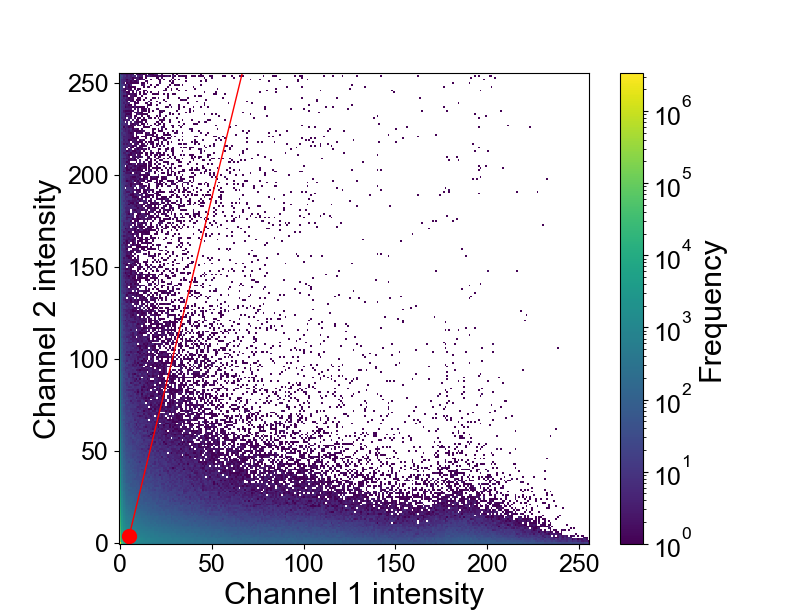
\includegraphics[width=0.49\linewidth]{figs/Placeholder_Image.png}}
    \subcaptionbox{The 3D intensity elevation projection of the image where the z-axis heights represent the pixel intensities \label{subfig:raw_3D}}{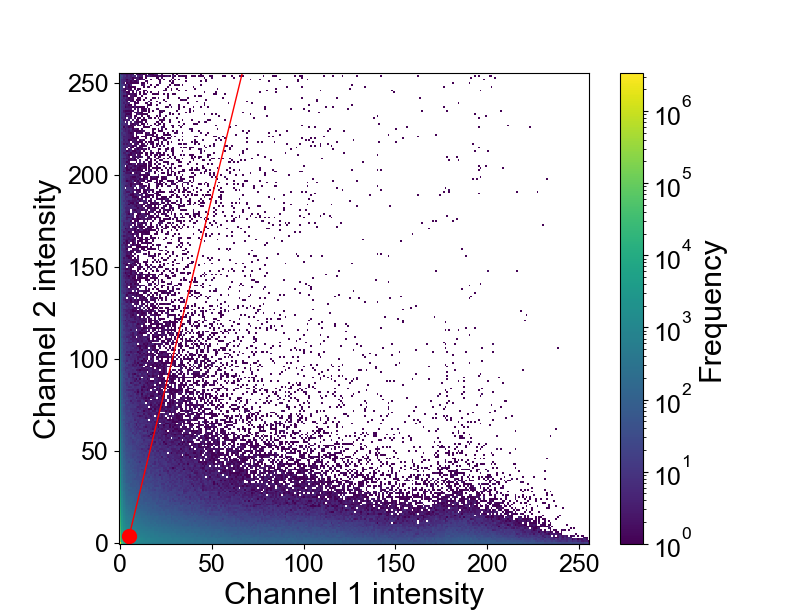
\includegraphics[width=0.49\linewidth]{figs/Placeholder_Image.png}}
    \subcaptionbox{The 2D image with the objects above and below the thresholds labelled. \label{subfig:hyst_labels_2D}}{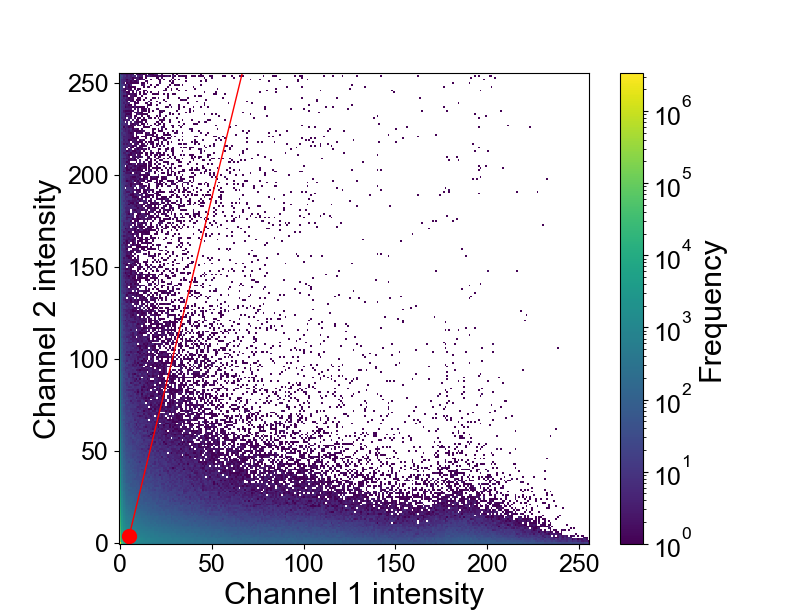
\includegraphics[width=0.49\linewidth]{figs/Placeholder_Image.png}}
    \subcaptionbox{The 3D representation with coloured labelling based on the thresholds \label{subfig:hyst_labels_3D}}{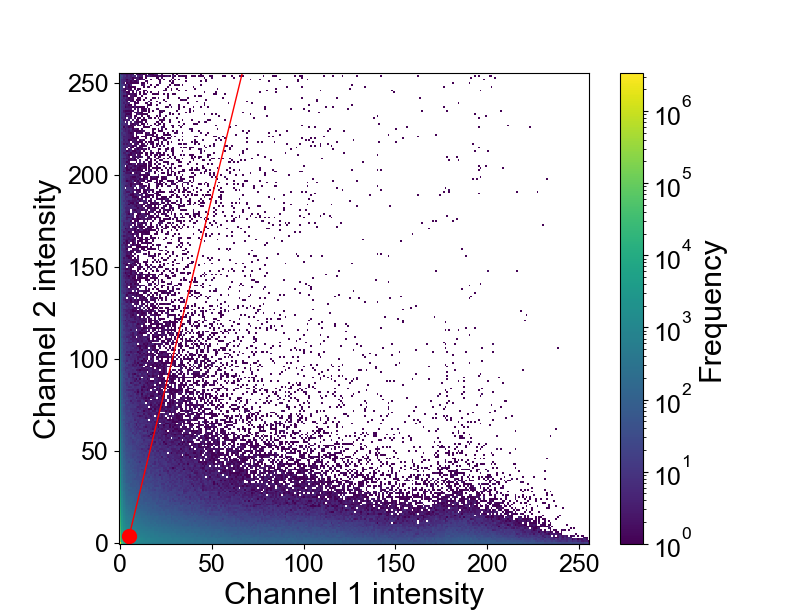
\includegraphics[width=0.49\linewidth]{figs/Placeholder_Image.png}}
    \subcaptionbox{The binarized 2D image of the regions that are preserved after Hysteresis is applied \label{subfig:hyst_applied_2D}}{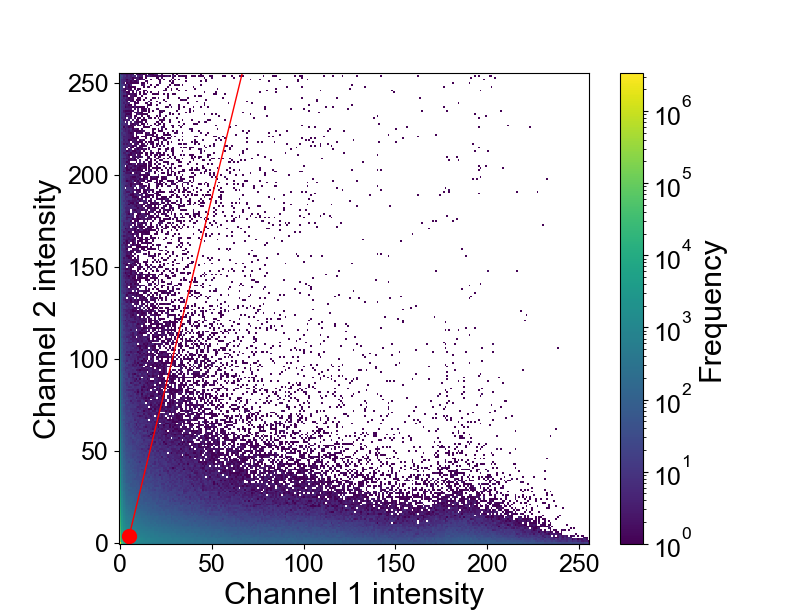
\includegraphics[width=0.49\linewidth]{figs/Placeholder_Image.png}}
    \subcaptionbox{The 3D intensity projection of the image after Hysteresis is applied. \label{subfig:hyst_applied_3D}}{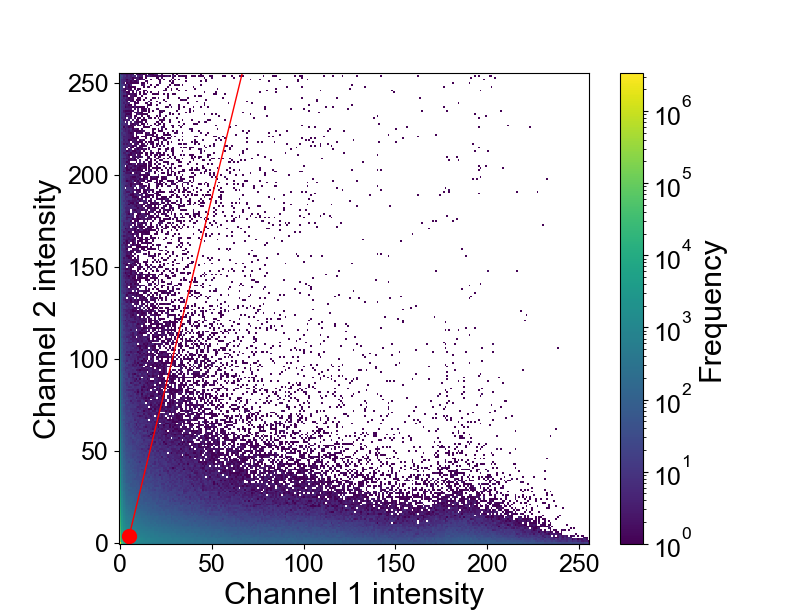
\includegraphics[width=0.49\linewidth]{figs/Placeholder_Image.png}}
    \caption[\textcolor{red}{This is currently not complete as 3D images are being a bit difficult and this is going to be moved to Chapter 2 (Hysteresis Section)}Showcasing the application of Hysteresis thresholding on a microscope image along with 3D intensity projections]{The application of Hysteresis thresholding is illustrating using an arbitrary 2D microscope image which is shown in sub-figures (\subref{subfig:raw_2D}), (\subref{subfig:hyst_labels_2D}), and (\subref{subfig:hyst_applied_2D}) while the 3D representation of each of these sub-figures are shown in (\subref{subfig:raw_3D}), (\subref{subfig:hyst_labels_3D}), and (\subref{subfig:hyst_applied_3D}) respectively. The Hysteresis labels applied in sub-figures (\subref{subfig:hyst_labels_2D}) and (\subref{subfig:hyst_labels_3D}) are selected based on what the pixel intensity is relative to the low and high thresholds with red representing pixels above the high threshold, green representing pixels between both thresholds and green representing pixels below the low threshold. Sub-figures (\subref{subfig:hyst_applied_2D}) and (\subref{subfig:hyst_applied_3D}) show the image after Hysteresis application with the results being binarized in the 2D representation (\subref{subfig:hyst_applied_2D}) while the 3D representation (\subref{subfig:hyst_applied_3D}) uses the binary output to mask the intensity image to improve clarity.}
    \label{fig:hysteresis_showcase_2D_3D}
\end{figure}
\subsection{Acquisition of the low threshold}\label{sec:low_acquis}
%Describe use of Kneedle (which should be discussed in theory in Chapter 2) and cite the github used for the software implementation. The use of the Normal and Log version (need to confirm that the log knee is always greater than the normal knee using data), and how Otsu is used to select the low threshold (picking between normal and log knee and compare both with Otsu thresh for why Otsu isn't used).
As has been described in Section \ref{sec:Hyst}, the low threshold is a crucial step in determining the quality of the Hysteresis thresholding outcome since it is the first threshold value deciding which voxels are background. This is important as the high threshold only acts on the remaining non-background voxels in the image thus a low threshold that is too low or too high results in either image noise that increases the difficulty of the high threshold selection or removes valuable regions of objects. Despite this, thresholding is a subjective operation frequently relying on the judgement of an expert to evaluate what is currently designated as background voxels in the image and whether they belong to an object of interest to the analysis.
\subsubsection*{Initial steps}
In the beginning, an investigation into robust and accurate low threshold estimators was performed but it was found that the established methods were lacking and for this reason established automated global threshold methods were considered. Automated global threshold methods had the benefit of not requiring parameter setting or tuning (aligning with a design objective of the system this research was developing) and there was a robust body of literature on these methods regarding their development. Many of these methods also were implemented in Python libraries thus the methods `Li', `Mean', `Otsu', `Triangle', and `Yen'~\cite{scikit-image} were tested. These methods were tested by application to the 25 sample images with the threshold results compared to the low threshold values selected by the experts.\paragraph{Initial findings} were that values chosen by `Li' or `Mean' were often far lower than the experts while `Yen' resulted in threshold values that diverged so greatly from all of the experts that Yen was omitted from further testing. Despite thresholding being a subjective evaluation, as mentioned prior, it is still ideal to achieve a closer value to the experts although how close, unfortunately, is image dependent. The remaining two methods, `Otsu' and `Triangle', were generally closer to the expert values although Otsu was generally closer to the experts.
%as can be seen in Table \ref{tab:results}.
\textcolor{red}{The table is empty for now as I need to determine if formatting functions well for horizontally long tables using tikz or tabular. For now, this is a placeholder and the boxplots visually describe this better (perhaps this should be moved to appendices?)}
\iffalse
\begin{table}
%A placeholder. If the sample data is too wide then the table will be generated as an image and then inserted. For now this will be where low threshold results will sit.
\begin{center}
\begin{tabular}{ |c|c|c| } 
 \hline
 cell1 & cell2 & cell3 \\ 
 cell4 & cell5 & cell6 \\ 
 cell7 & cell8 & cell9 \\ 
 \hline
\end{tabular}
\end{center}
\caption{\textcolor{red}{This is currently still a placeholder as I am determining a) if the formatting will work for the full numeric results; and b) whether they should rather be moved to the appendices as the box plot explains it better}\label{tab:results}}
\end{table}
\fi
This is visually described in Figure \ref{fig:expert_boxplot} where the overlaid box plot and strip plots represent the difference between each thresholding method and the experts for each sample. Although this is not a perfect comparison as each sample is technically unique to each other and this comparison is reductionist in that it does not consider the conditions of each image that lead to certain results but this can serve as an estimation of the sensitivity of the performance of the thresholding methods and how robust they are to a range of image conditions. As these comparisons regard the difference between the threshold method and the expert results tending towards zero are better as they are more similar to the expert with Figures \ref{subfig:thresh_diff} and \ref{subfig:vox_diff} describing the difference between the threshold value and the number of foreground voxels respectively. Although it was already established that Otsu and Triangle were the best-performing threshold methods there is confirmation of this with the threshold value difference (Fig. \ref{subfig:thresh_diff}) where Otsu has larger quartile ranges than that of Triangle but with the distribution of sample values more closely centred on the zero line. What this means is that Otsu experiences greater swing in performance across samples yet when it does perform well it performs better that Triangle yet Triangle is more consistent in outcome although this outcome is slightly worse. Image thresholding remains a highly subjective and image-dependent evaluation and for this reason, although still an unsatisfactory measure of overall performance, an evaluation in the binarization output per sample (Fig. \ref{subfig:vox_diff}) is to be explored. This difference in foreground voxel counts shows that save for Expert A, Otsu has greater consistent similarity to the experts although the shortcoming is that when it deviates it can deviate strongly. When this analysis was conducted there was also an evaluation of the binarization outcome on the samples between the thresholding methods and the experts although only these reductive comparisons have been shown as they serve as effective approximations of the binarization results across a large body of samples. What was determined is that although these methods could provide passable results, the impact of poorly selected low thresholds can render a binarization outcome useless for analysis, if not detrimental if uncaught, thus an alternative thresholding method is required.
\begin{figure}
    \centering
    \subcaptionbox{Difference between the low threshold determined by the automated method and the experts\label{subfig:thresh_diff}}{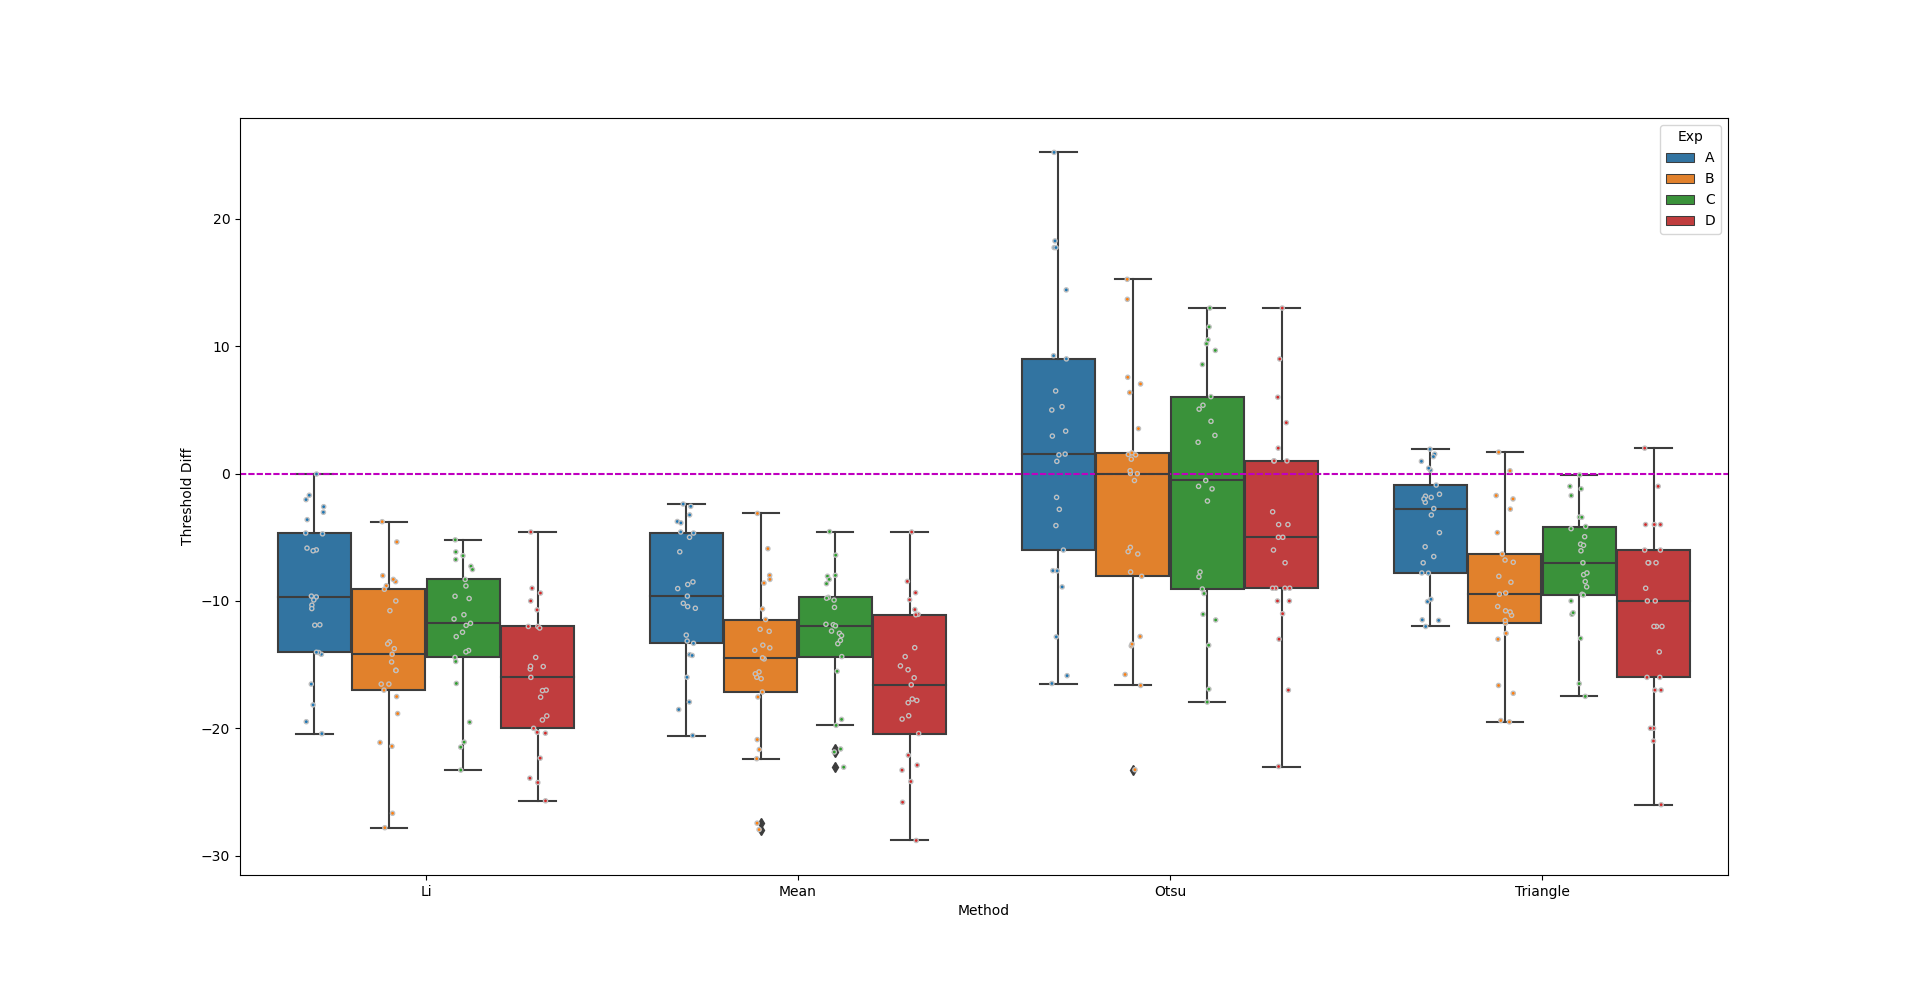
\includegraphics[width=\textwidth]{figs/ch3figs/Thresh_diff.png}}
    \subcaptionbox{Difference in non-background voxel count between the automated methods and the experts\label{subfig:vox_diff}}{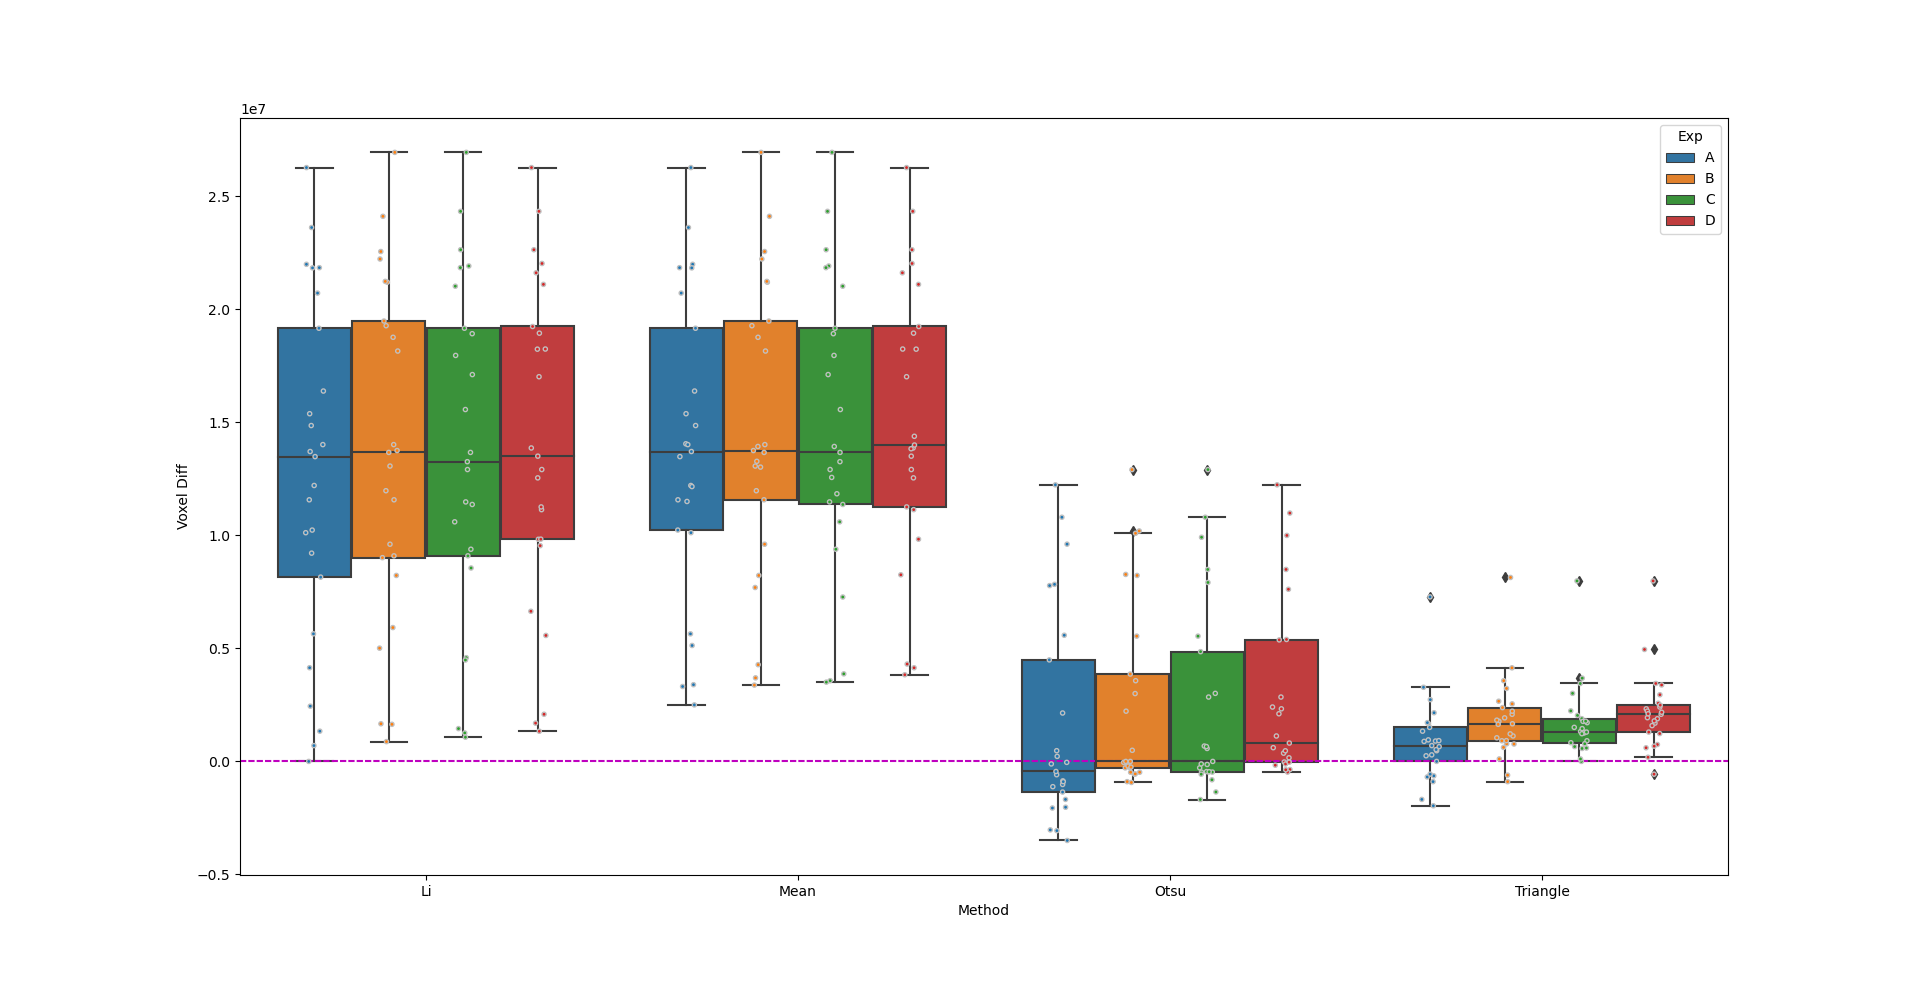
\includegraphics[width=\textwidth]{figs/ch3figs/Vox_diff.png}}
    
    \caption[Difference between expert values and automated thresholding results in terms of the threshold value and binarization outcome]{Difference between expert values and automated thresholding results in terms of the threshold value and binarization outcome depicted using box plots overlaid with strip plots. These plots describe the difference between the thresholding method and the experts for each sample where (\subref{subfig:thresh_diff}) represents the difference in the numeric threshold value while (\subref{subfig:vox_diff}) represents the difference in the count of the foreground image pixels. As greater similarity is preferred the goal is a value of zero denoted by a dashed magenta line on both sets of plots.}
    %Caption needs to be improved
    \label{fig:expert_boxplot}
\end{figure}
\paragraph{The alternative} thresholding method that was decided on was an application of the `Kneedle' algorithm (Section \ref{sec:kneedle}) where elbows within the image histogram are to be used as the low threshold. The motivation for this decision was based on comparisons between the expert-selected low thresholds and where they are positioned on the image histogram as it was hypothesised that there is some low-intensity region of the histogram that would represent the image background. The challenge surrounding this was, once again, that image binarization is a subjective process where typically some value can be estimated and based on its impact on the binarization it is further tuned. Despite this, it was hypothesised that there must be some baseline which would generally be agreed upon by experts regardless of the results. This baseline was formulated from four notions being:
\begin{enumerate}
    \item That there will always be a background within the image, as there must be two states to differentiate between with binarization, where the background will be comprised of voxels with intensities ranging from the lowest in the image up to, or below, the lowest foreground intensity.
    \item While the upper bound of the background intensity range is uncertain initially, the lower bound is well-defined. Given this, there is complete certainty that the lowest intensity belongs to the background but this does not hold true for consecutively greater intensity values.
    \begin{description}
        \item[Note:] This background upper bound is uncertain in ``lower quality'' images where there is no clear separation between the background and foreground modes due to either noise or other irregularities.
    \end{description}
    \item The background is composed of two potential ``groups'' of the background of which the lower intensity is referred to as the `empty' background and the high intensity is the `irregular' background. The term potential was used as the `empty' background is always present and this is the background voxels that do not describe any objects within the image but rather is the absence of any observable objects or phenomena which typically exist in a small near homogeneous intensity range. This composes the space between the foreground objects in the image but there is another group of backgrounds which can appear during unwanted imaging conditions which is the `irregular' background. 
    \begin{description}
        \item[Note:] This `irregular' background is an umbrella term for the background elements in the image composed of fluorescence signals which are unwanted for the analysis or were not intended to be captured, e.g. a small amount of a bio-molecules autofluorescence emission is within the filtered spectra and thus is included appearing as a faint shadow. This fluorescence is referred to as irregular as it does not follow noise models nor is it distinct enough to typically present as foreground objects thus it is irregular with respect to what is supposed to, or expected to, compose the image background. 
    \end{description}
    
    \item With pre-processing applied it is expected that background induced by noise will be near homogeneous and describe some ``empty background'' where no actual or false objects are depicted and exhibit among the lowest intensity values in the image. From this, our certainty is highest among the lowest intensities where the ``empty background'' is situated and diminishes as the voxel intensities originate from irregular background conditions.
    \begin{description}
        \item[Note:] This view was motivated by evaluations of the image histograms and the impact of the low threshold values on the image by image analysis. This was depicted by a high peak spanning a narrow range of intensity values centred at the lowest histogram values.  
    \end{description}
\end{enumerate}
Based on these notions a theoretical framework was established which can be referred to as the ``low-intensity background confidence'' where the confidence that an intensity value belongs to the background is relative to how low the intensity is and that the confidence for an intensity value cannot be greater than any lower intensity values e.g. if we are $A$ confident that voxels of intensity $x$ belongs to the background and $B$ confident that voxels of an intensity $x+1$ belong to the background then $A \geq B$ must hold true for the confidence. Despite this algebraic example, the confidence is closer to that of an informed intuition instead of some known distribution of function. Regardless, our most confident background selection lay from where the low-intensity peak significantly flattened in slope and thus a method to approximate this best point of plateau became necessary. This does not imply that all voxels of an intensity greater than this point do not belong to the background but rather were deemed to be a point which would sufficiently capture the majority of the noise which would be most impactful to the binarization as the low threshold determined the volume and joining of potentially foreground objects and since the ``empty background'' constituted the space between the foreground, insufficient binarization could induce the erroneous joining of foreground structures.
\textcolor{red}{Should I include some (say two) example histograms where I annotate where the low-intensity peak in the histogram lies?}
\iffalse
\begin{figure}
%The 3D images here need to be labelled based on ndi_labels and then spread across 255 to get a colour range. An inset for a specific region of interest should be shown as well
    \centering
    \subcaptionbox{3D intensity projection of all pixels above low threshold A\label{subfig:low_thresh_A}}{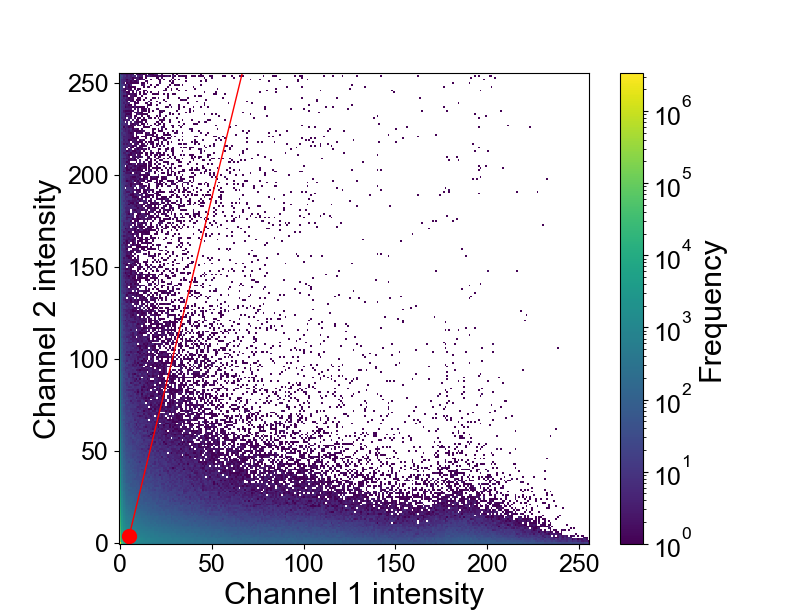
\includegraphics[width=0.49\linewidth]{figs/Placeholder_Image.png}}
    \subcaptionbox{3D intensity projection of all pixels above low threshold B\label{subfig:low_thresh_B}}{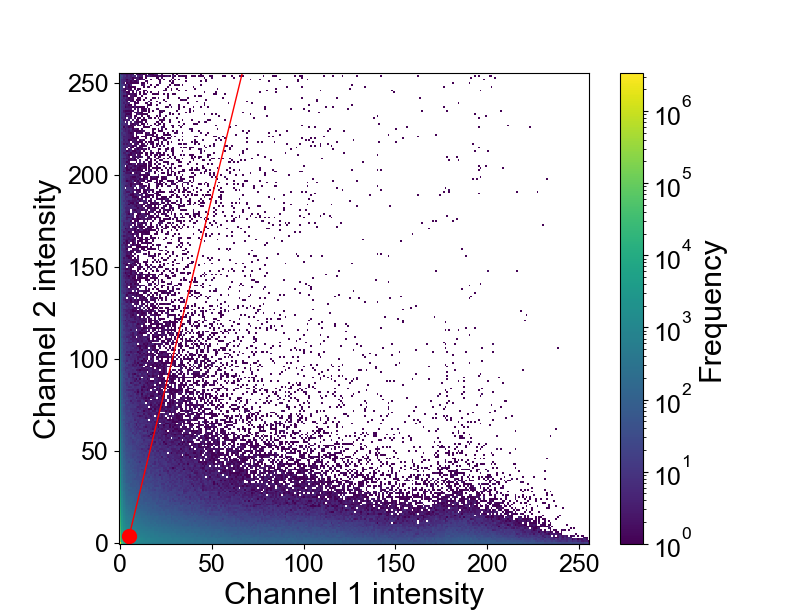
\includegraphics[width=0.49\linewidth]{figs/Placeholder_Image.png}}
    \caption[The outcome of the selected low threshold on area and separation of independent regions]{The outcome of the selected low threshold on area and separation of independent regions. The raw image is shown in Figure \ref{subfig:raw_3D} while both of the figures here (\subref{subfig:low_thresh_A}) and (\subref{subfig:low_thresh_B}) have different low thresholds of values A and B applied respectively where B is a low threshold value than A. \subref{subfig:low_thresh_A}) has smaller areas for the regions and which are also more separated, while in \subref{subfig:low_thresh_B}) the areas are larger yet previously separated regions are joined as shown in the annotated area of interest.}
    \label{fig:my_label}
\end{figure}
\fi
\subsubsection{Using Kneedle for low threshold approximation}\label{sec:low_thresh_kneedle}
%First, mention how Kneedle (ref the section) can be used to determine some turning point after a steep drop. Secondly, mention how this parts with our postulations where we will have some inital peak related to the background mode centred around the lowest background value (the size of the peak may vary but it is almost always there). Thirdly, mention how the log elbow was determined as a point to help with scenarios where it was fear to be too low. Lastly, mention the current selection criteria involving Otsu and the pros vs cons of it. There will be a single figure which will have the metric closeness and the voxel count closeness between Elbow, Log Elbow, Otsu, and Triangle.
The ``Kneedle'' algorithm (Section \ref{sec:kneedle}) is applied to the image histogram with the goal of approximating a sufficiently low threshold such that at least all of the `empty' background is captured within its range. This relies on the fact that Kneedle can determine either the knees or elbows within a function which can be characterised as the point of most sudden change in the gradient of the function after either increasing or decreasing respectively. For this application, the `empty' background is assumed to always be described by some crest among the lowest intensity values and it is the fall from this crest that is of interest. It was only after the application of this method and the evaluation of the binarized regions, regarding what it was certain was background from what might be foreground, that the effectiveness was observed. While the method at times fell short of the Expert values it frequently excluded the `empty' background values at least and was found to generally perform well. This can be seen in Figure \ref{fig:elbow_expert_compare} which compares the performance of the Kneedle low threshold, as well as Otsu and Triangle for reference as the prior best performers, to the Experts. While this comparison is reductive as it does not evaluate what is being binarized in the image (objects, shapes or patterns typically are passed through for evaluation by the High threshold) since it is a linear threshold it is known that if two thresholds are identical then their impact on the image binarization will be identical. From the results, it is seen that the results acquired by Kneedle are closer to the Experts across the span of samples and that the variance in the performance is tighter describing a more reliable outcome which is easier to predict. What may be noticed is that there is also a mention of ``Log Kneedle'' in both figures as well as ``Chosen Kneedle''.\paragraph{Log Kneedle} is the low threshold elbow that is acquired using the log of the histogram as opposed to the normal histogram. This application was hypothesised based on the notion that taking the log of the histogram will normalize and rescale it allowing the higher-intensity histogram components to be discerned if they have been drowned out by a huge `empty' background peak which can result in low threshold values that are too low. This is applicable as this log normalization allows large changes in the `empty' background, irregular background, and potential foreground intensity range to be evaluated in the histogram typically resulting in a higher elbow for the low threshold. Looking at Figure \ref{subfig:thresh_elbow} and \ref{subfig:voxel_elbow} it can be seen that the results of the Log Kneedle are highly varied in performance, particularly so for Expert A which also performed the worst, but its perspective on irregular background presence that the `empty' background might overshadow was believed to hold merit but not in the current approach.\paragraph{The Chosen Kneedle} was the approach which was established to tune whether to get the normal or log-transformed low threshold under some criteria. The criteria that were chosen were that if the Otsu threshold exceeded that of the Kneedle elbow then the log Kneedle elbow would be used instead. This was under the assumption that Otsu will be a poor performer given that the image quality resulted in the foreground and background modes being difficult to separate. The primary motivation behind this was that there were times when both the normal Kneedle elbow value and the Otsu value were too low leading to a greater amount of `empty' background being retained and diminishing the robustness of the high threshold approximation. This was a stopgap solution though and it cannot be reduced that the log Kneedle elbow value will be necessarily closer to the Experts but rather there is a significantly lower risk of `empty' background retention and the value still remains constrained.\textcolor{red}{I am slightly uncertain how to end this section. I feel that there is a distinct difference in the impact of both the Chosen and Normal Kneedle value although based on the similarity with the experts Normal appears to perform better but for cases where there is too much noise the normal incorrectly retains the chosen Kneedle is better. I could place a reference to Chapter 4 where the impact of each on the overall performance is evaluated?}
\iffalse
The 'Kneedle' algorithm (Section \ref{sec:kneedle}) is able to approximate turning points in distributions that are either \textit{knees} or \textit{elbows} where the elbow after the aforementioned low-intensity peak in the image histograms might be a sufficiently low threshold estimate. While this might not be the optimal low threshold in all samples particularly where the noise present persists into higher intensity ranges a slightly higher low threshold might be preferred but after manual evaluation over the 25 samples mentioned prior it was determined that in most cases it performed reasonably. This is supported by the results depicted in Figure \ref{fig:elbow_expert_compare} where in Fig. \ref{subfig:thresh_elbow} `Elbow Normal' can be seen to have a complete quartile range tighter than Otsu yet similar to Triangle meaning there is less variance in the difference from the experts than exhibited in Otsu. By observing the median line, where 50\% of sample values are situated above and below said line across the quartiles, it can be seen that in `Elbow Normal' the difference results typically skew in the direction of the zero line such that if the median is below zero then there is a positive skew meaning a greater proportion of those two quartile range values are closely situated around zero. In Fig. \ref{subfig:voxel_elbow} it can be seen that the `Elbow Normal' quartile distribution remains far tighter than that of Otsu and, surprisingly, Triangle although the median line positioning means that the skew tends towards zero strongly for only Expert A and C while only an outer quartile situates to zero for Expert B and D. Comparitively, Otsu only has noticeable skew with Experts B and C where the Median line lies on zero thus 
\fi
\begin{figure}
    \centering
    \subcaptionbox{Difference in threshold metric to be applied as the Hysteresis low threshold\label{subfig:thresh_elbow}}{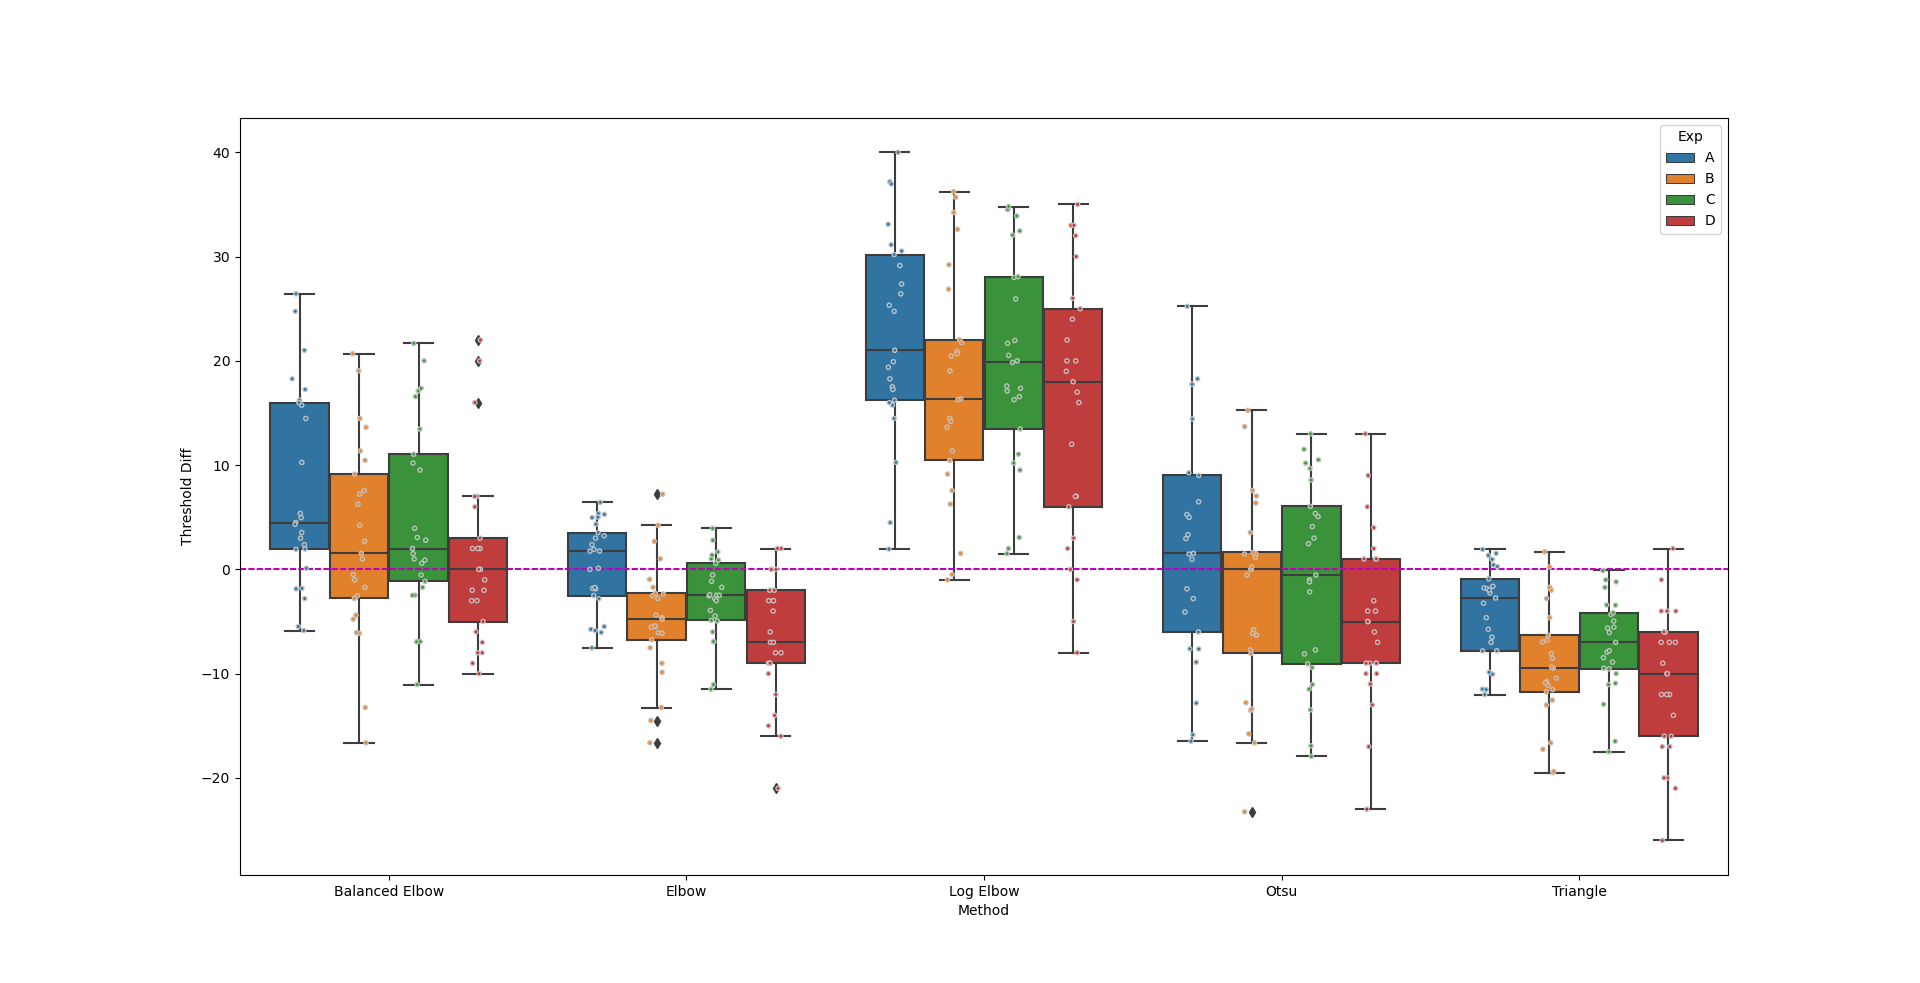
\includegraphics[width=0.49\textwidth]{figs/ch3figs/Knee_Thresh_diff.png}}
    \subcaptionbox{Difference in voxel count post-binarization using the threshold value as the image would appear after low threshold application\label{subfig:voxel_elbow}}{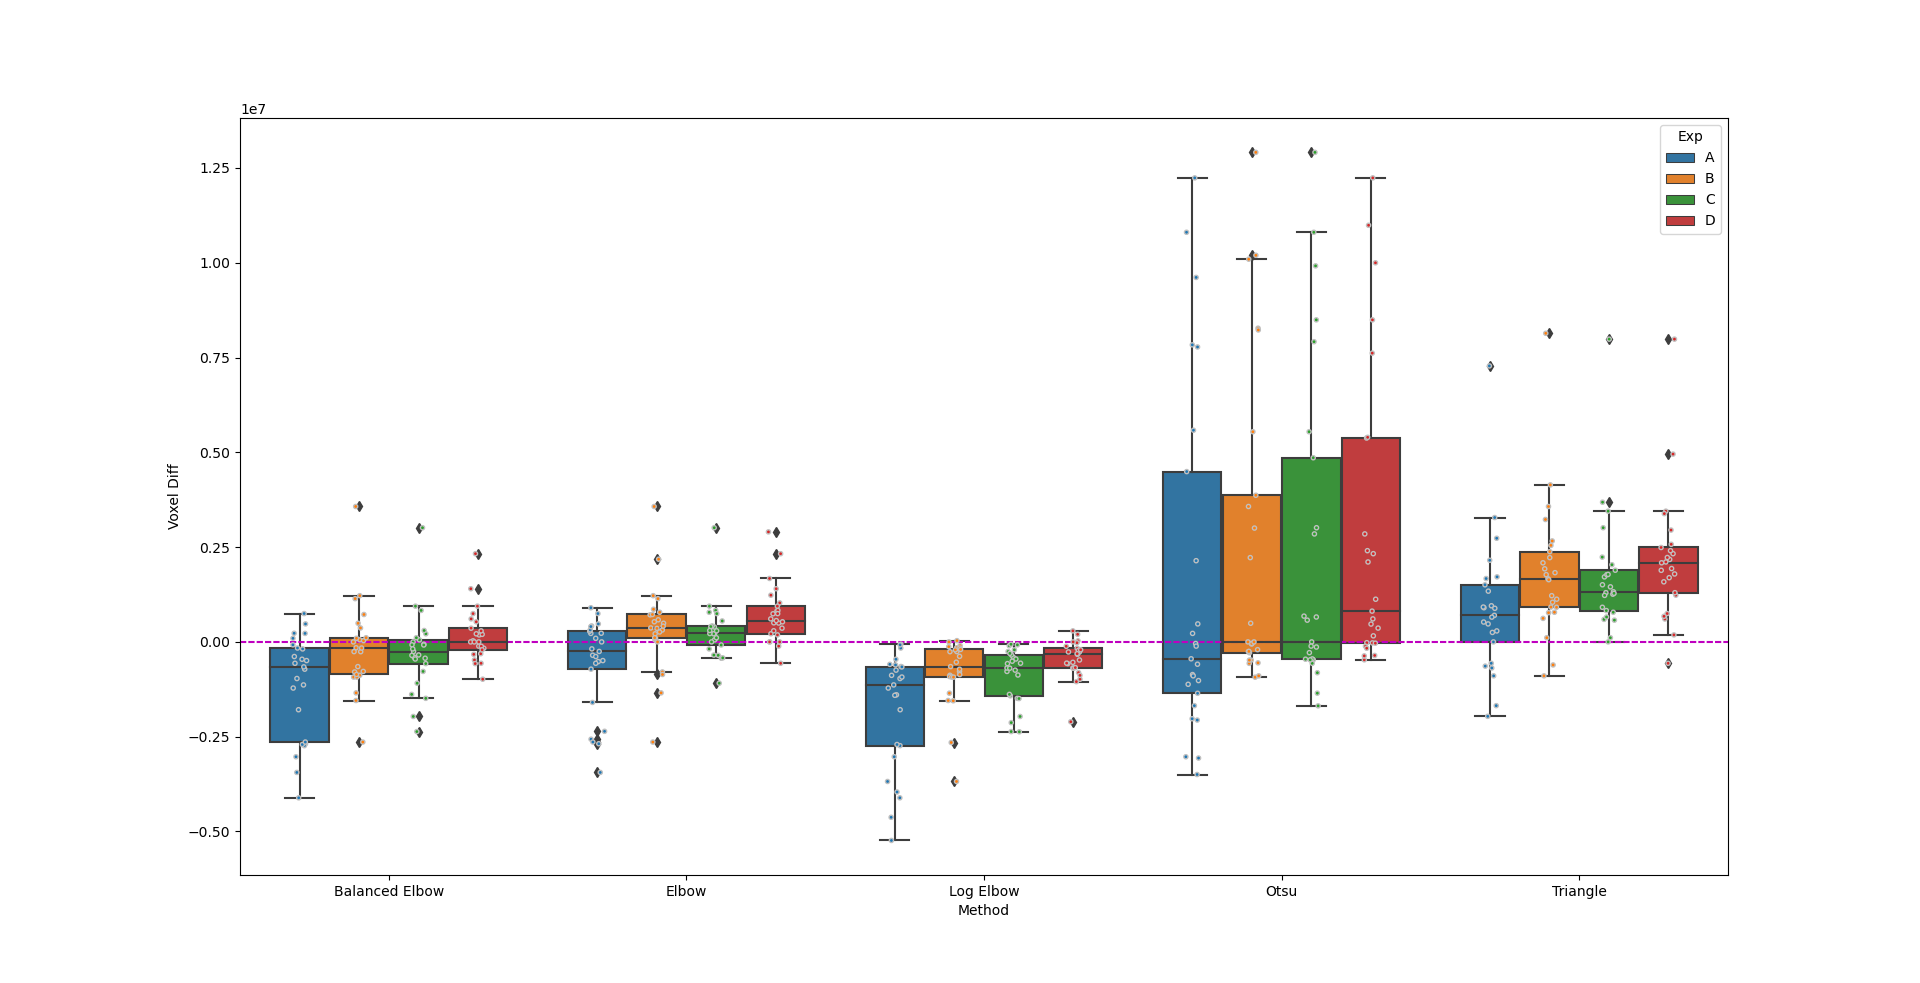
\includegraphics[width=0.49\textwidth]{figs/ch3figs/Knee_Vox_diff.png}}
    \caption[Comparison between the thresholding method and the Experts for Otsu, Triangle, normal Elbow, log Elbow, and the chosen Elbow]{Comparison between the thresholding method and the Experts for Otsu, Triangle, normal Elbow, log Elbow, and the chosen Elbow. This comparison is depicted using box plots to describe the variance in the difference between the experts across multiple samples and the simplified distribution of these values.}
    \label{fig:elbow_expert_compare}
\end{figure}
\iffalse
The application of Kneedle to determine a low threshold was based on the hypothesis that selecting a low threshold around the elbow of the histogram would be able to remove the majority of the low intensity in the image. It was found though that at certain times the determined elbow would be sufficient for threshold use while at other times the determined elbow was too low of a value. For reference a human selected low threshold for each sample was chosen that was used to compare the ideal estimated low threshold compared to what was determined. In a fair number of samples it was found that the determined elbow was too low of a value (significantly lower than the expert selected low threshold) and an approach was required to determine a closer value while not fixating on the expert's exact value as it recognised that the value would be determined subjectively by the expert. Simultaneously it was speculated that although the exact value selected by an expert was subjective there would be underlying components informing that decision and perhaps these objective components could be inferred from the histogram. To better visualise the complete histogram and evaluate where structural information is present within the intensity range the logarithm of the histogram was implement in the elbow approximation. After some brief observations of a small subset of samples a second hypothesis was formulated that calculating the elbow of the log of the histogram could determine an elbow higher in value than before but not out of realistic range for a sample compared to the expert. After some tests this hypothesis was partially fulfilled particularly where the elbow of the normal histogram was found to be far lower than the desired low threshold.% Stipulate that the log was an earlier exploration of the histogram from a suggestion made during a disucssion with Rensu Theart
\par The final problem lay in selecting which elbow to use of either the normal histogram elbow or the log histogram elbow without prior knowledge of which elbow would be more desirable for a given sample. Tests with the Otsu threshold were performed to compare with the respective Kneedle results (normal and log) to investigate if the values could act as some form of decision criteria between the two elbow options. These tests were performed and the comparison between the elbow results produced by the Kneedle algorithm \cite{kneedle_arvai}; the Otsu, Mean, Yen and Triangle thresholds in scikit-image \cite{scikit-image}; and the threshold values manually determined by an expert. Using this comparison it was observed that when the Otsu threshold was greater than the normal histogram elbow that the log histogram elbow was a closer threshold value to that selected by the expert while an Otsu value less than or equal to the normal histogram elbow occurred when the normal histogram elbow was closer to the threshold value selected by the expert. To evaluate the performance of this a test was performed involving a reference threshold which was generated for each image using expert low and high thresholds which was compared to images of the same corresponding samples but the low threshold was determined using one of the aforementioned automated methods. The automated threshold images used an automated low threshold determined by the Triangle, Otsu or best fit elbow method while the high threshold used for the image was still the expert high threshold such that only the relative impact of the low threshold was evaluated. The measure used to compare these partially automated threshold images and the expert reference image is the structural image overlap similarity measure described in Section \ref{sec:similarity_metric}. From Fig. \ref{subfig:low_boxplot} it can be seen that while the Otsu and Knee results share the same median value the interquartile range of the Knee results are not as wide as that of the Otsu results thus there is greater consistency in the performance of the Knee results across the tested samples. While the Triangle results have the narrowest interquartile range it is observed that the median similarity metric is the lowest and the upper quartile is lower than both the Otsu and Knee upper quartiles. In Fig. \ref{subfig:low_mean} the height of the bars depict the average similarity measure for each threshold measure across the test sample range. Of these average similarity results it is seen that the Knee threshold achieve a greater average similarity than the other threshold methods. Further analysis of these results is discussed in Section \ref{sec:low_thresh_metrics} but what can be summarised is that the selective Kneedle algorithm produces threshold images that achieve the highest similarity on average, have the highest minimum similarity across the sample set and provide the second most consistent results based on the interquartile range. %Need to also do a comparison comparing chosen vs normal vs log to determine why it is best to select the knee approach
\begin{figure}[h!]
    \centering
    \subcaptionbox{Sample histogram of the complete intensity range\label{subfig:noisy_hist}}{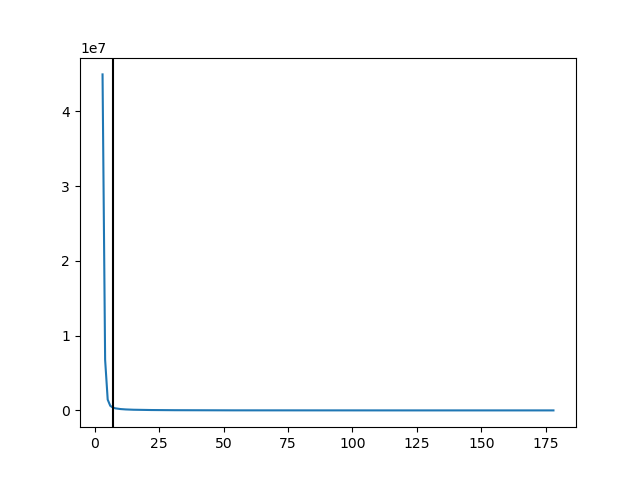
\includegraphics[width=0.48\linewidth]{figs/hist.png}}
    \subcaptionbox{Sample histogram with an intensity range from the low intensity elbow to the maximum}{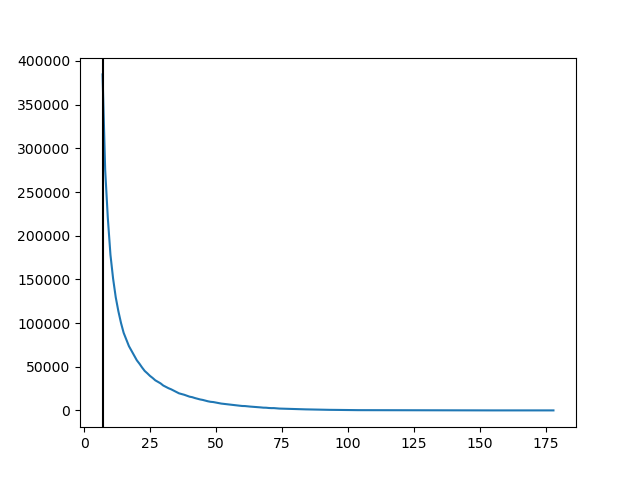
\includegraphics[width=0.48\linewidth]{figs/hist_cut.png}}
    \subcaptionbox{The log representation of the sample histogram for the full intensity range}{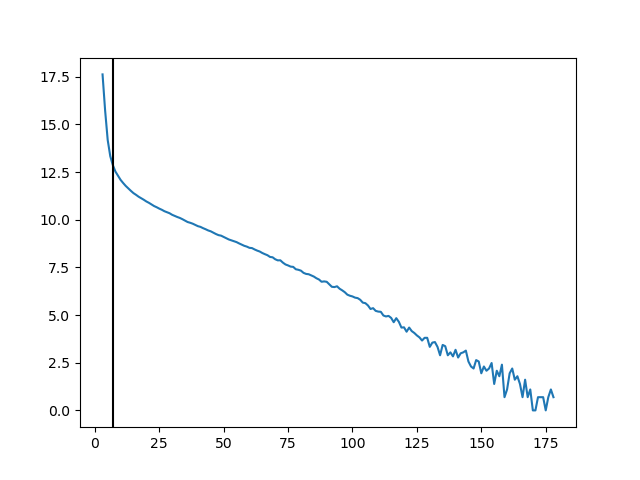
\includegraphics[width=0.48\linewidth]{figs/hist_log.png}}
    \subcaptionbox{The log representation of the sample histogram for the intensity range from the original histogram low intensity elbow}{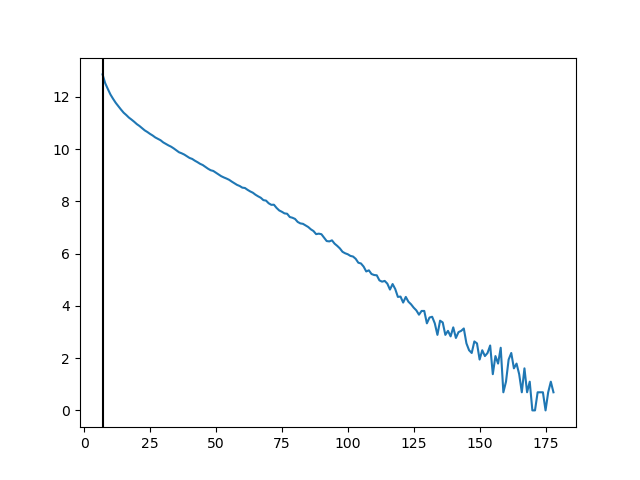
\includegraphics[width=0.48\linewidth]{figs/hist_log_cut.png}}
    \caption{Sample histograms of the intensity frequency across the intensity range. A black vertical line designates the estimated elbow of the histogram}
    \label{fig:sample_hist_for_low}
\end{figure}
\fi
\newpage
\subsection{High threshold acquistion}
With the low threshold for a given sample image selected the final step is to approximate a suitable high threshold value. While the low threshold approximation was also challenging the high threshold was a more complex problem due to the image histogram being comparatively less useful. While images with clearly depicted foreground and background modes in the histogram allow for the high threshold to be selected, relative to the foreground mode, this is not the case in images where the foreground mode is unclear. This is typically due to either out-of-focus fluorescence, higher-intensity noise components not removed by denoising, unexpectedly stained biomolecules (e.g. free-floating proteins in the Cytoplasm), or image artefacts. The former two are addressed by deconvolution and denoising respectively during pre-processing although when the presence is too strong there may be interferences remaining, particularly with noise as overly aggressive denoising can degrade the image signal, yet the latter two cannot be addressed as easily with most methods although appropriate image thresholding is one of the means to address this. The reason for this is that many thresholding methods can be tuned to preserve the actual foreground objects in the image while both rejecting the remainder as background and minimizing image signal degradation. The images worked with in this research exhibit all four of the aforementioned obstructions, in different severities, to effectively separate the foreground and background modes thus a means of estimating an optimal labelling of foreground objects. \paragraph{Design considerations made for foreground acquisition} were important to make as this method could not rely on some known perfect output but rather had to find some result which provided the best-estimated outcome. There were three primary considerations that were made which are:
\begin{enumerate}
    \item The system must adapt to each image to get an image-specific outcome but apply identical logic to all of them
    \item Image attributes used in the system must relate to the intensities of the potential foreground voxels
    \item If the system makes an error then it must be done in a manner that is the least detrimental to future analysis
\end{enumerate}
To address these considerations intensity-related attributes such as the pixel/voxel intensity distribution visualised by the histogram and intensity distributions across pixel neighbourhoods were raised. The primary problem with these is that utilizing the voxel intensity distribution across the image encounters the same problems of mode separation which confronts global threshold methods while neighbourhood-based approaches where the intensity distribution is aggregated encounter the parameter selection obstacles of local threshold methods where the size of the neighbourhood, among other parameters, directly affects performance. Since the low threshold had already been resolved a method that evaluates only the impact of the high threshold was required and led to a hypothesis that if the impact of the high threshold on the image across a threshold range could create a distribution then perhaps that could describe other image features?

\subsection{Iterative hysteresis histogram (IHH)}\label{sec:ihh}
%Define an acronym for this IHH and how this is constructed by iterating the high threshold until it equals the low thresh for hysteresis and the number of retained voxels is counted.
This method was termed iterative hysteresis histogram (IHH), which is a distribution relating to the high threshold hysteresis application but also the name of the method by which it is acquired. This distribution is the total count of potential foreground voxels at each high threshold where the high threshold ranges from 1 intensity above the low threshold up to the maximum image intensity. An example illustrating the approach used to construct the IHH is shown in Figure \ref{fig:ihh_sequence} where a microscope maximum intensity projection (MIP) image is used for illustrative purposes. This culminates in a distribution that begins at \underline{one above} the low threshold intensity with some maximum count $X$ which is a non-increasing function $f(x)$ which can either remain the same or decrease as $x$ increases (where $x$ is the high threshold value). Due to this non-increasing nature of the function, the largest magnitude of $f(x)$ will be at the lowest possible $x$ value (one above the low threshold) and the shape of $f(x)$ across the intensity range can describe certain image properties. This distribution across the high threshold range can describe the foreground `confidence' of structures within the image as higher intensities are more likely to compose the foreground as the intensity tends towards the maximum intensity (similar to the background confidence baseline described at the end of Section \ref{sec:low_acquis}). The reason for this confidence is that voxel intensities within the image are chiefly dependent on how in-focus the emitting fluorophores are implying that it is highly likely that the depth at which the captured fluorescence originates aligns with the depth described in the image and that there is a reasonably high density of fluorophores at that position such that the increased density of fluorescence originating from said point result in a higher combined intensity value in the image. This assumption functions as a heuristically based justification for this confidence but is not the sole reason and only functions under the assumption that the quality at which the image is captured is sufficient such that foreground and background separation can be performed using visual analysis performed by a human. As illustrated in Figure \ref{fig:ihh_contrast_compare} an image with a well-separated foreground and background has a more rectangular IHH (Fig. \ref{subfig:mip_good_contrast_ihh}. \& \subref{subfig:rectangular_ihh}. for MIP and IHH respectively) where the high peak in count in the highest intensities depicts that a large proportion of the structures persist from a strict high threshold and only a few additional structures appear at the lower intensities. The opposite is seen in the poorly separated foreground and background (Fig. \ref{subfig:mip_bad_contrast_ihh}. \& \subref{subfig:sloping_ihh}. for MIP and IHH respectively) where the sloping nature of the IHH reflects the dispersion of the structures across the range of intensity values increasing the difficulty in evaluating what is and is not of the foreground in the image. The challenge is that there are few algorithmic ways in which to quantify the shape of the IHH and consistent logic by which to evaluate it compared to some metric such as standard deviation or variance for example.  

\begin{figure}
%This will be a sequence of images to show how the IHH is determined. 1. The raw MIP; 2. The MIP with bordering around the structures; 3. The structures colour coded to show the independent volumes; 4. The colouring changed to match the brightest pixel in the structure and a legend denoting that; 5. The IHH with vertical lines annotating where certain structures appear at. If borders cannot be placed then ignore 2.
    \centering
    \subcaptionbox{Raw MIP of a microscopy image\label{subfig:raw_mip_sequence}}{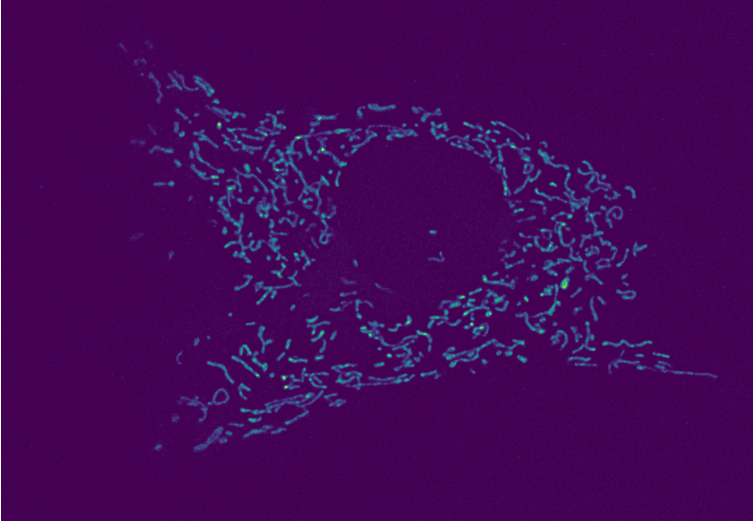
\includegraphics[width=0.32\textwidth]{figs/ch3figs/Before_Hyst.png}}
    \subcaptionbox{Structures labelled using unique colours for differentiation\label{subfig:colour_coded_sequence}}{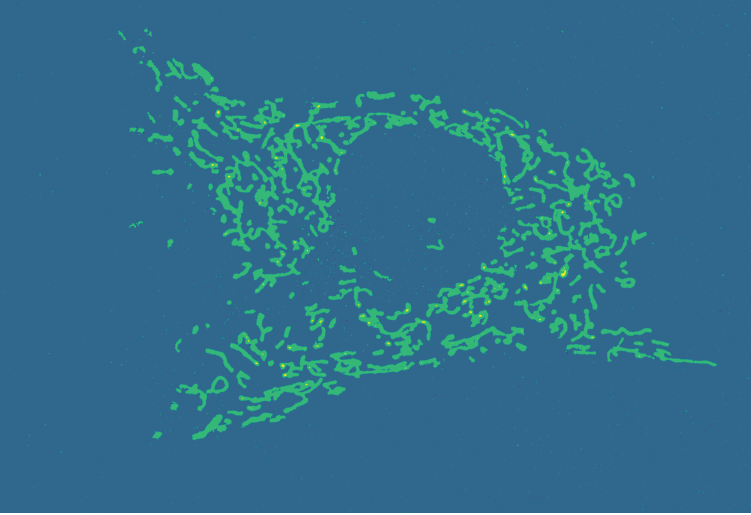
\includegraphics[width=0.32\textwidth]{figs/ch3figs/Mid_Hyst.png}}
    \subcaptionbox{Structures coloured based on brightest contained pixel intensity\label{subfig:pixel_intensity_sequence}}{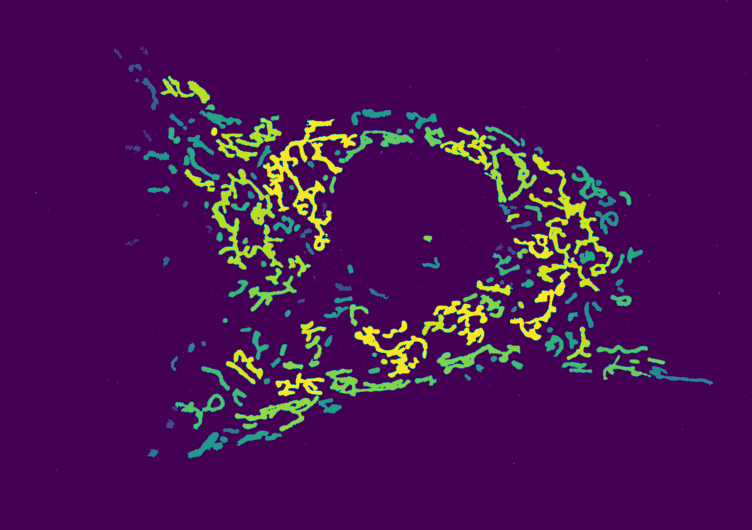
\includegraphics[width=0.32\textwidth]{figs/ch3figs/Intensity_labels.png}}
    \subcaptionbox{IHH of image with annotations regarding the highest intensity possessed by each structure\label{subfig:annotated_ihh_sequence}}{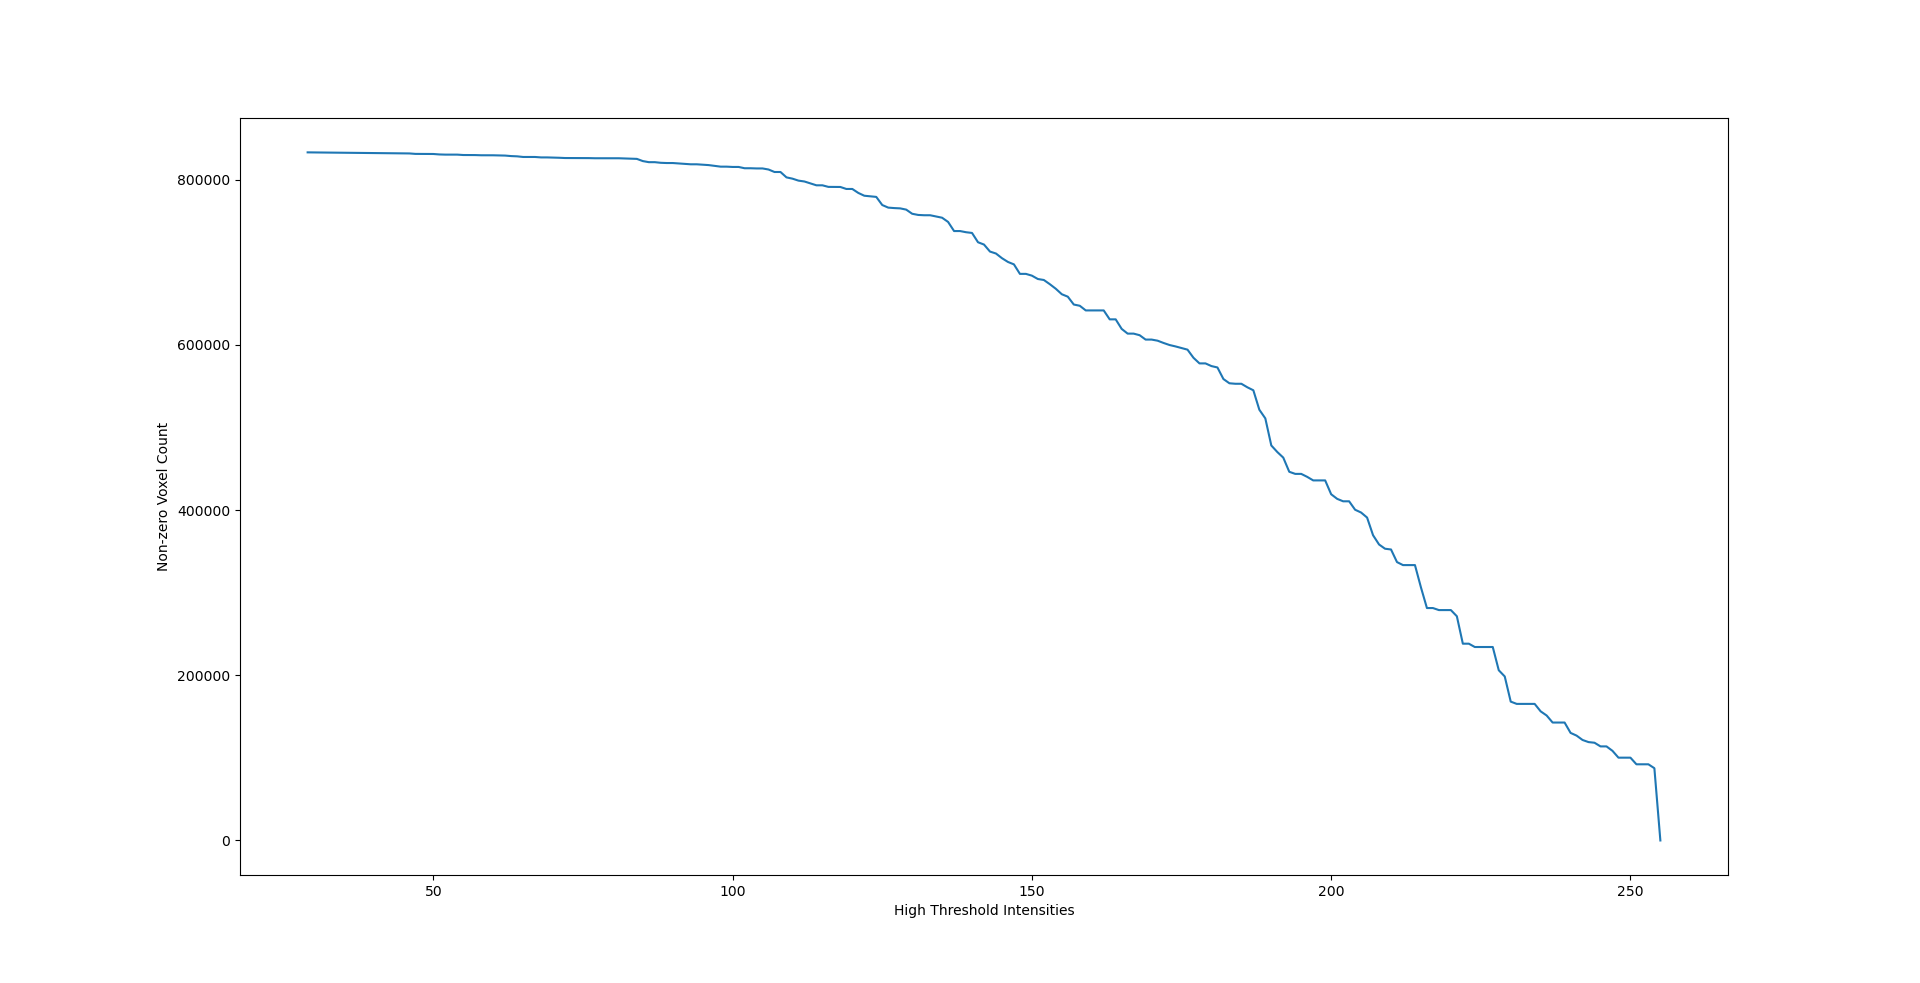
\includegraphics[width=\textwidth]{figs/sample_ihh.png}}
    \caption[An illustration of the sequence by which the IHH is determined for a cell image]{\textcolor{red}{The IHH in Figure \ref{subfig:annotated_ihh_sequence} is supposed to have colour coding that matches the structure colours in \ref{subfig:pixel_intensity_sequence}}An illustration of the sequence by which the IHH is determined for a microscopy cell image. The image used is a 2D maximum intensity projection of an original 3D image for illustrative purposes. This depicts how \textbf{\subref{subfig:raw_mip_sequence})} the raw image appears initially; \textbf{\subref{subfig:colour_coded_sequence})} the labelling of the independent structures in the image which are labelled by both colour and a numeric annotation; \textbf{\subref{subfig:pixel_intensity_sequence})} the structures are now re-coloured based on the highest pixel intensity contained within it which is also reflected in the annotated labels; \textbf{\subref{subfig:annotated_ihh_sequence})} lastly, the IHH that is constructed from the sum of the volumes of each structure from the lowest intensity up until their respective maximum.}
    \label{fig:ihh_sequence}
\end{figure}
\begin{figure}
    \centering
    \subcaptionbox{MIP of well separated foreground and background \label{subfig:mip_good_contrast_ihh}}{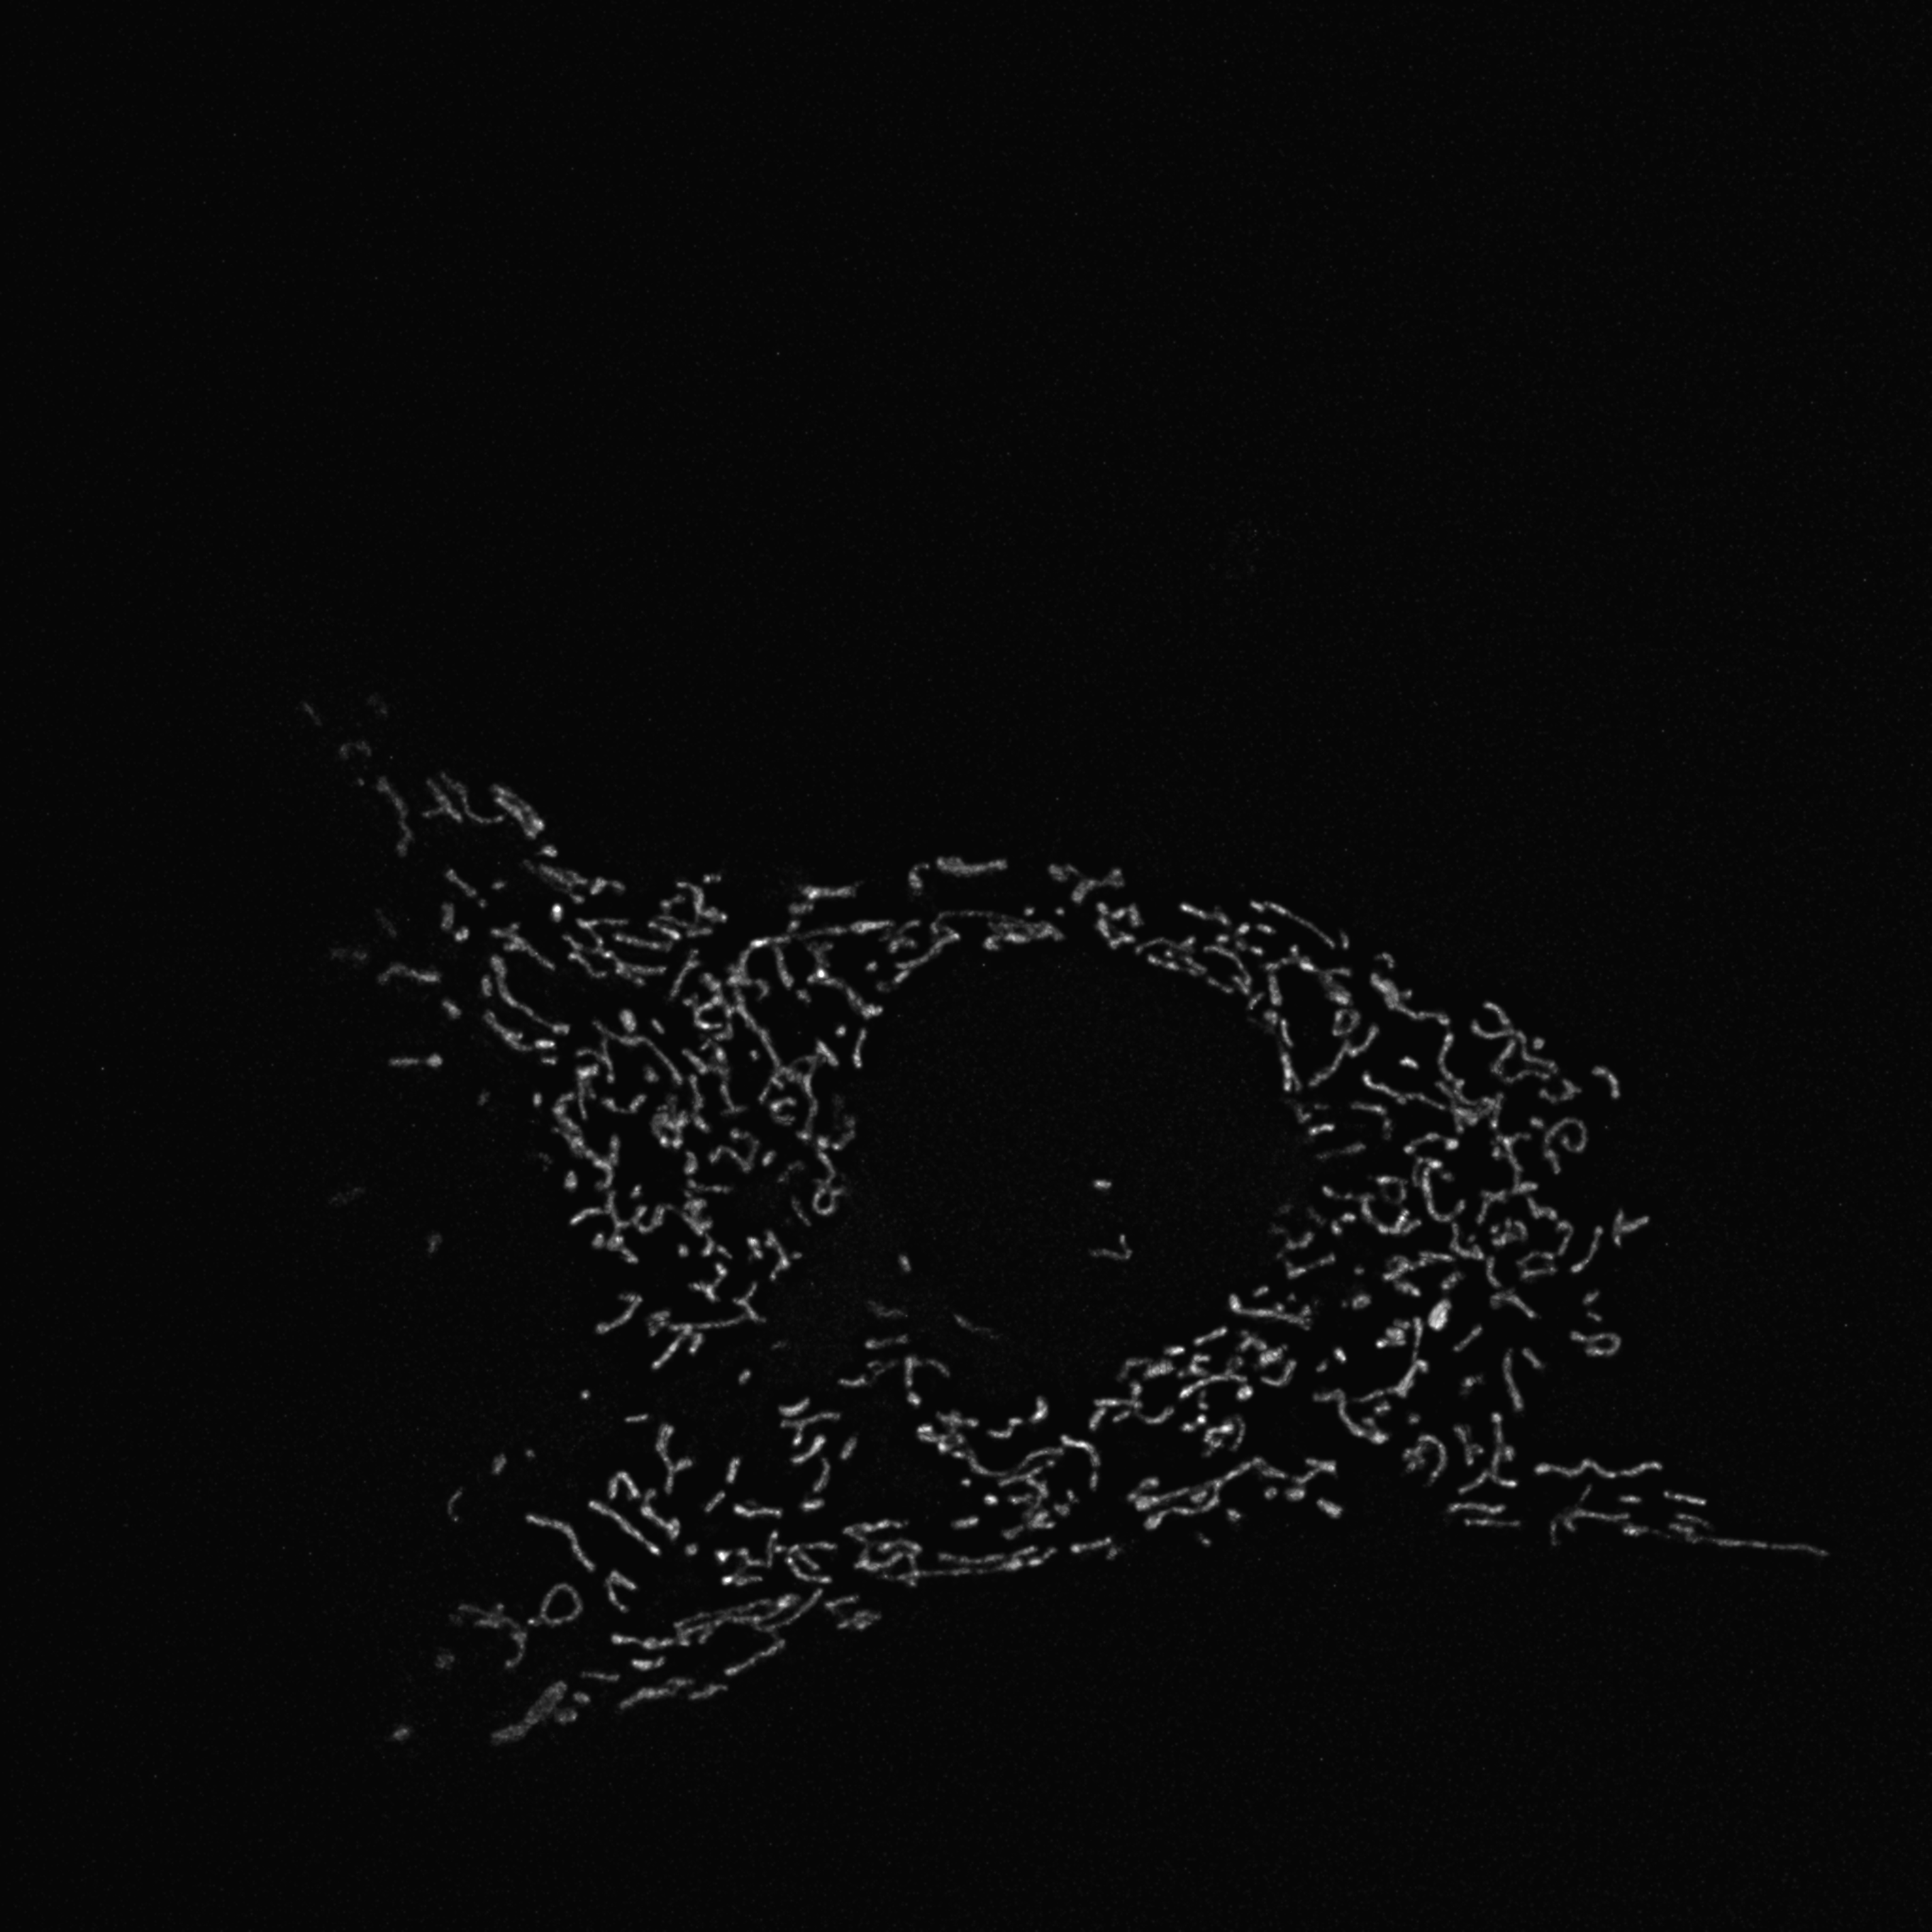
\includegraphics[width=0.49\textwidth]{figs/ch2figs/CCCP_1C=1T=0_normal.png}}
    \subcaptionbox{IHH of \subref{subfig:mip_good_contrast_ihh}) \label{subfig:rectangular_ihh}}{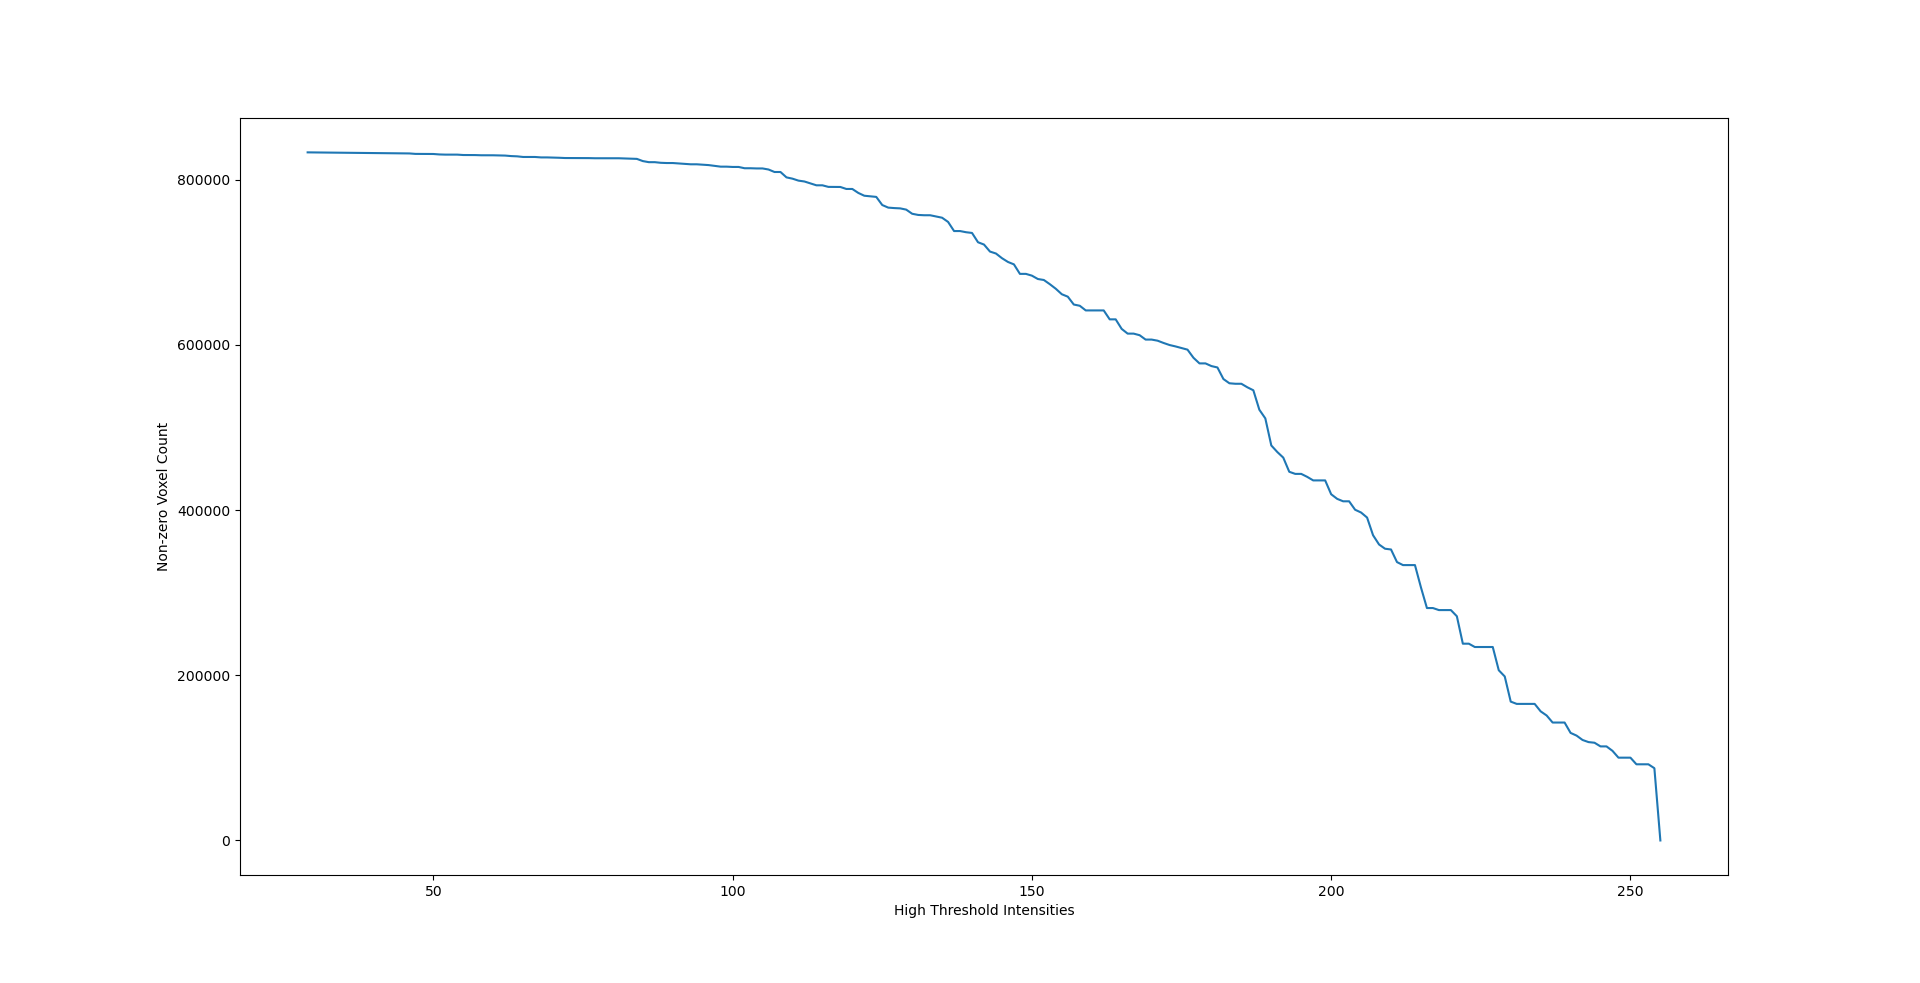
\includegraphics[width=0.49\textwidth]{figs/sample_ihh.png}}
    
    \subcaptionbox{MIP of poorly separated foreground and background \label{subfig:mip_bad_contrast_ihh}}{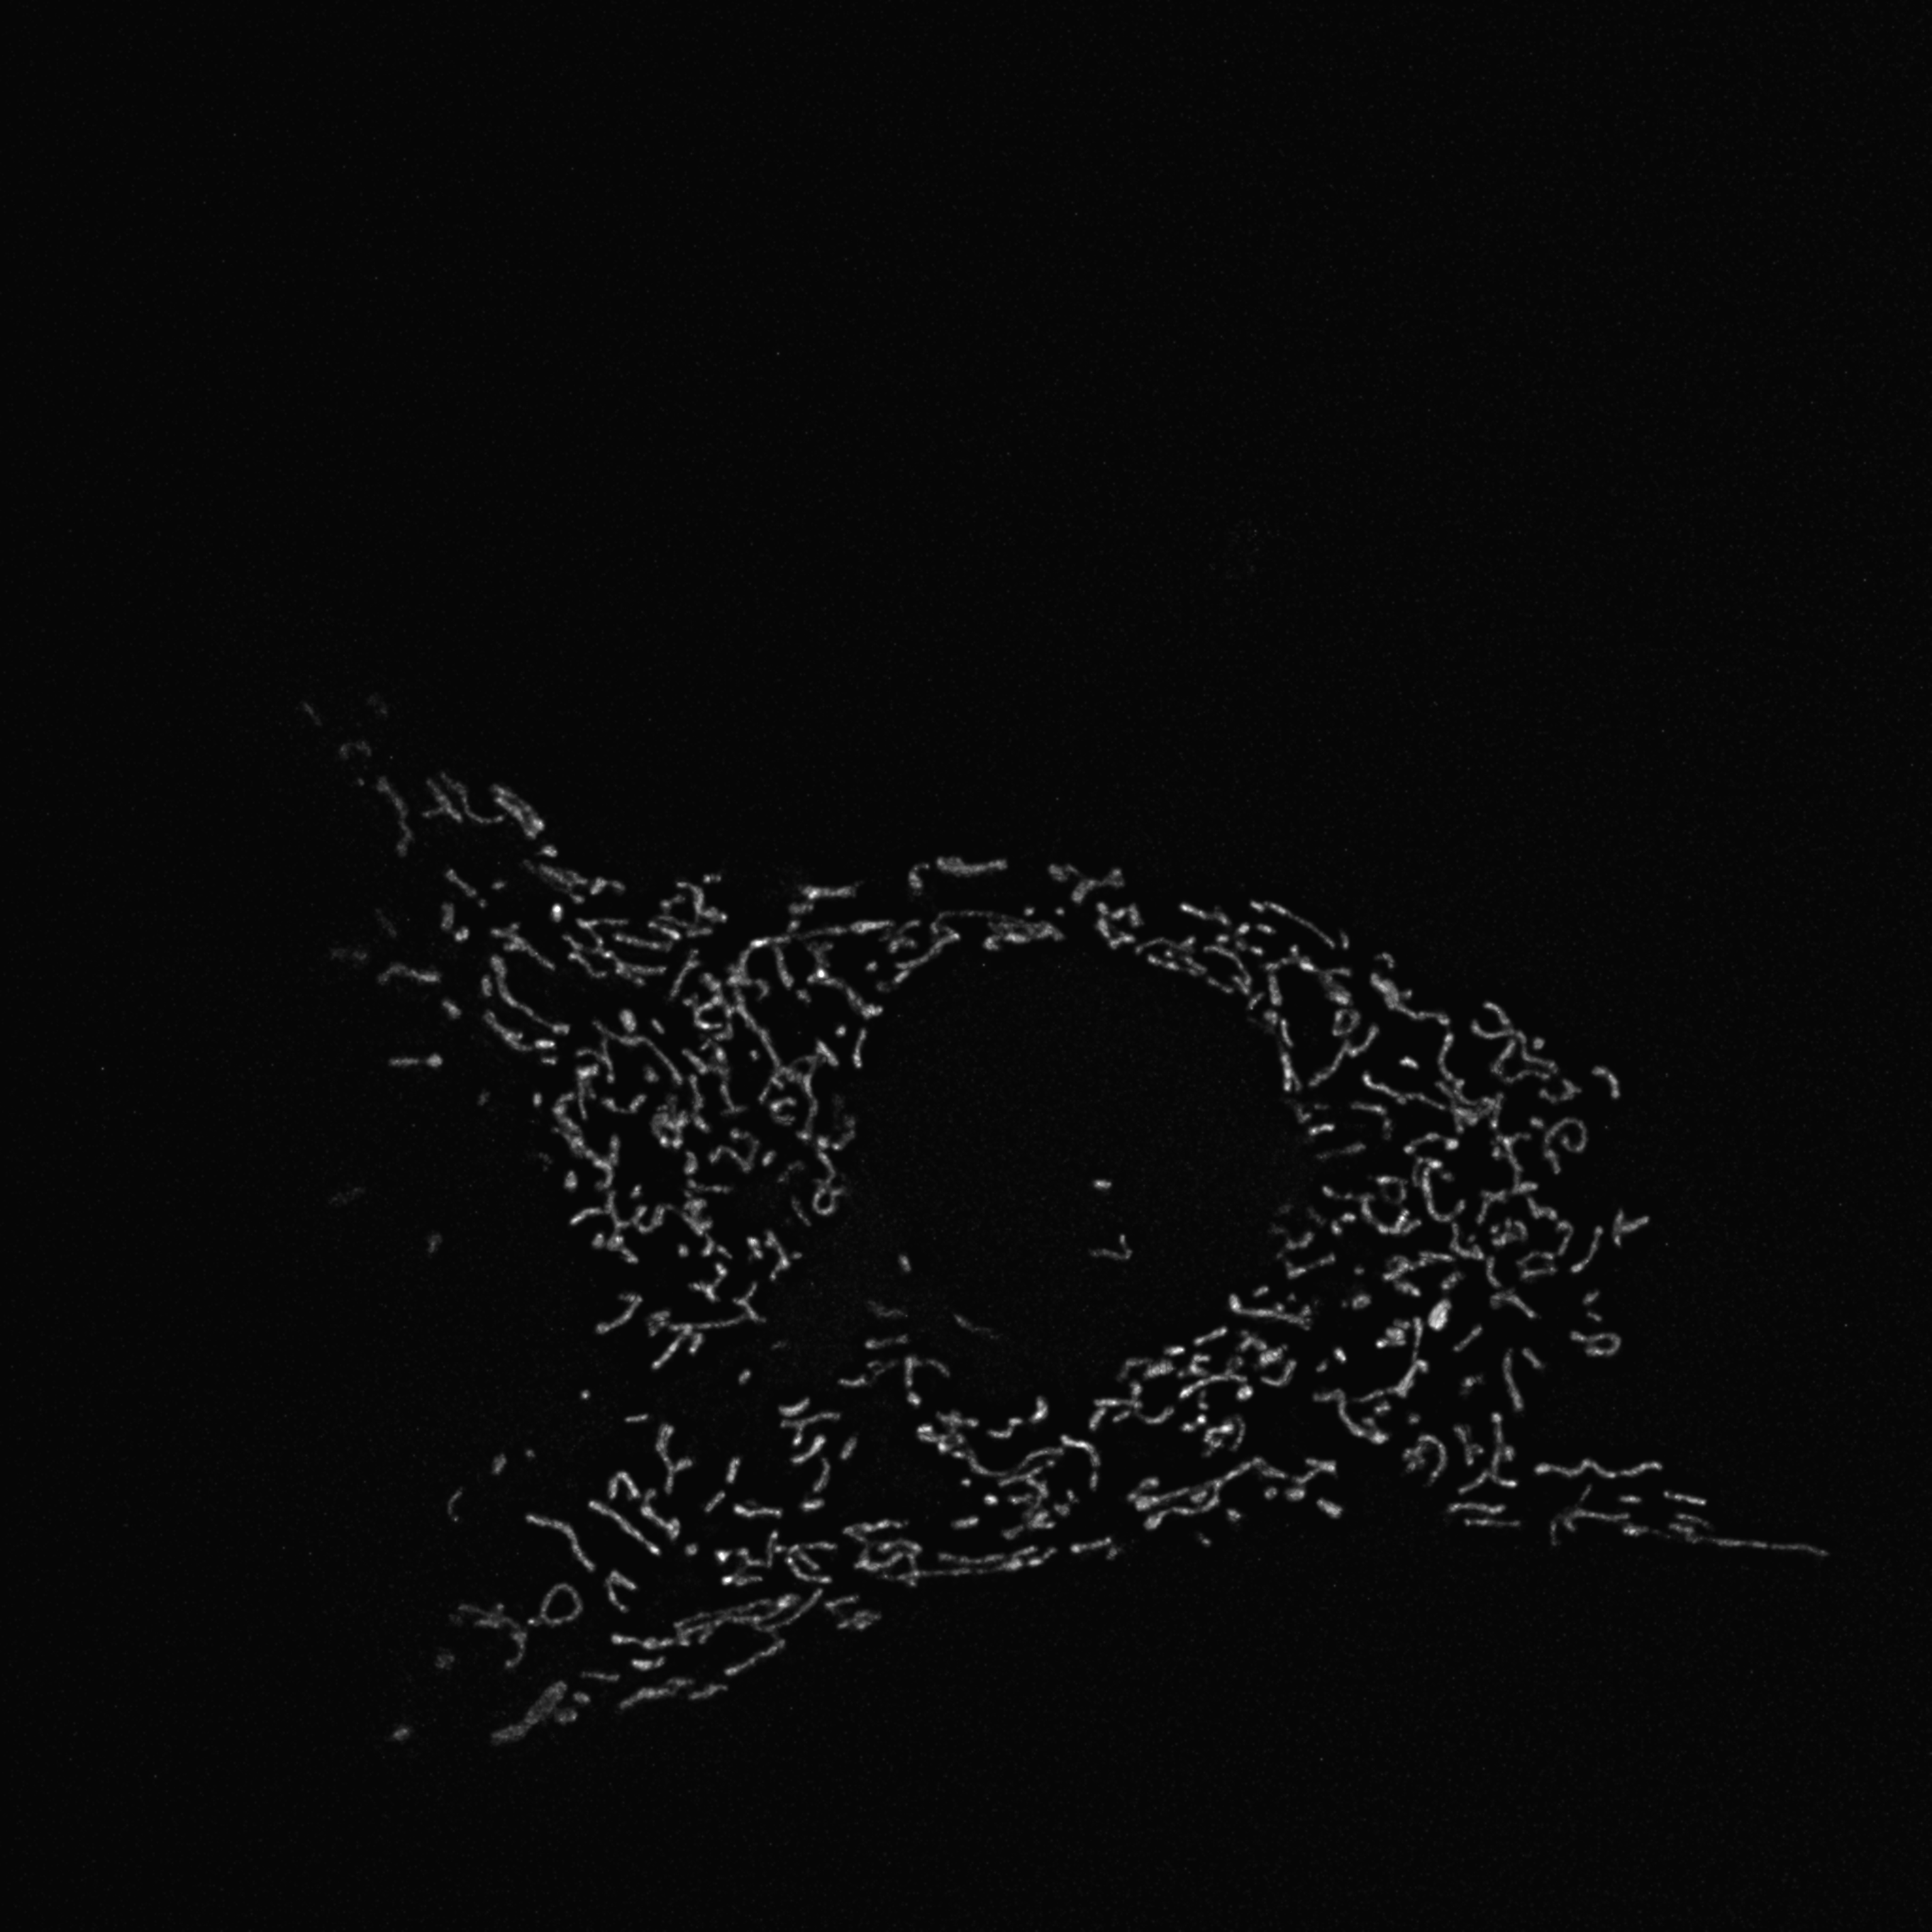
\includegraphics[width=0.49\textwidth]{figs/ch2figs/CCCP_1C=1T=0_normal.png}}
    \subcaptionbox{IHH of \subref{subfig:mip_bad_contrast_ihh}) \label{subfig:sloping_ihh}}{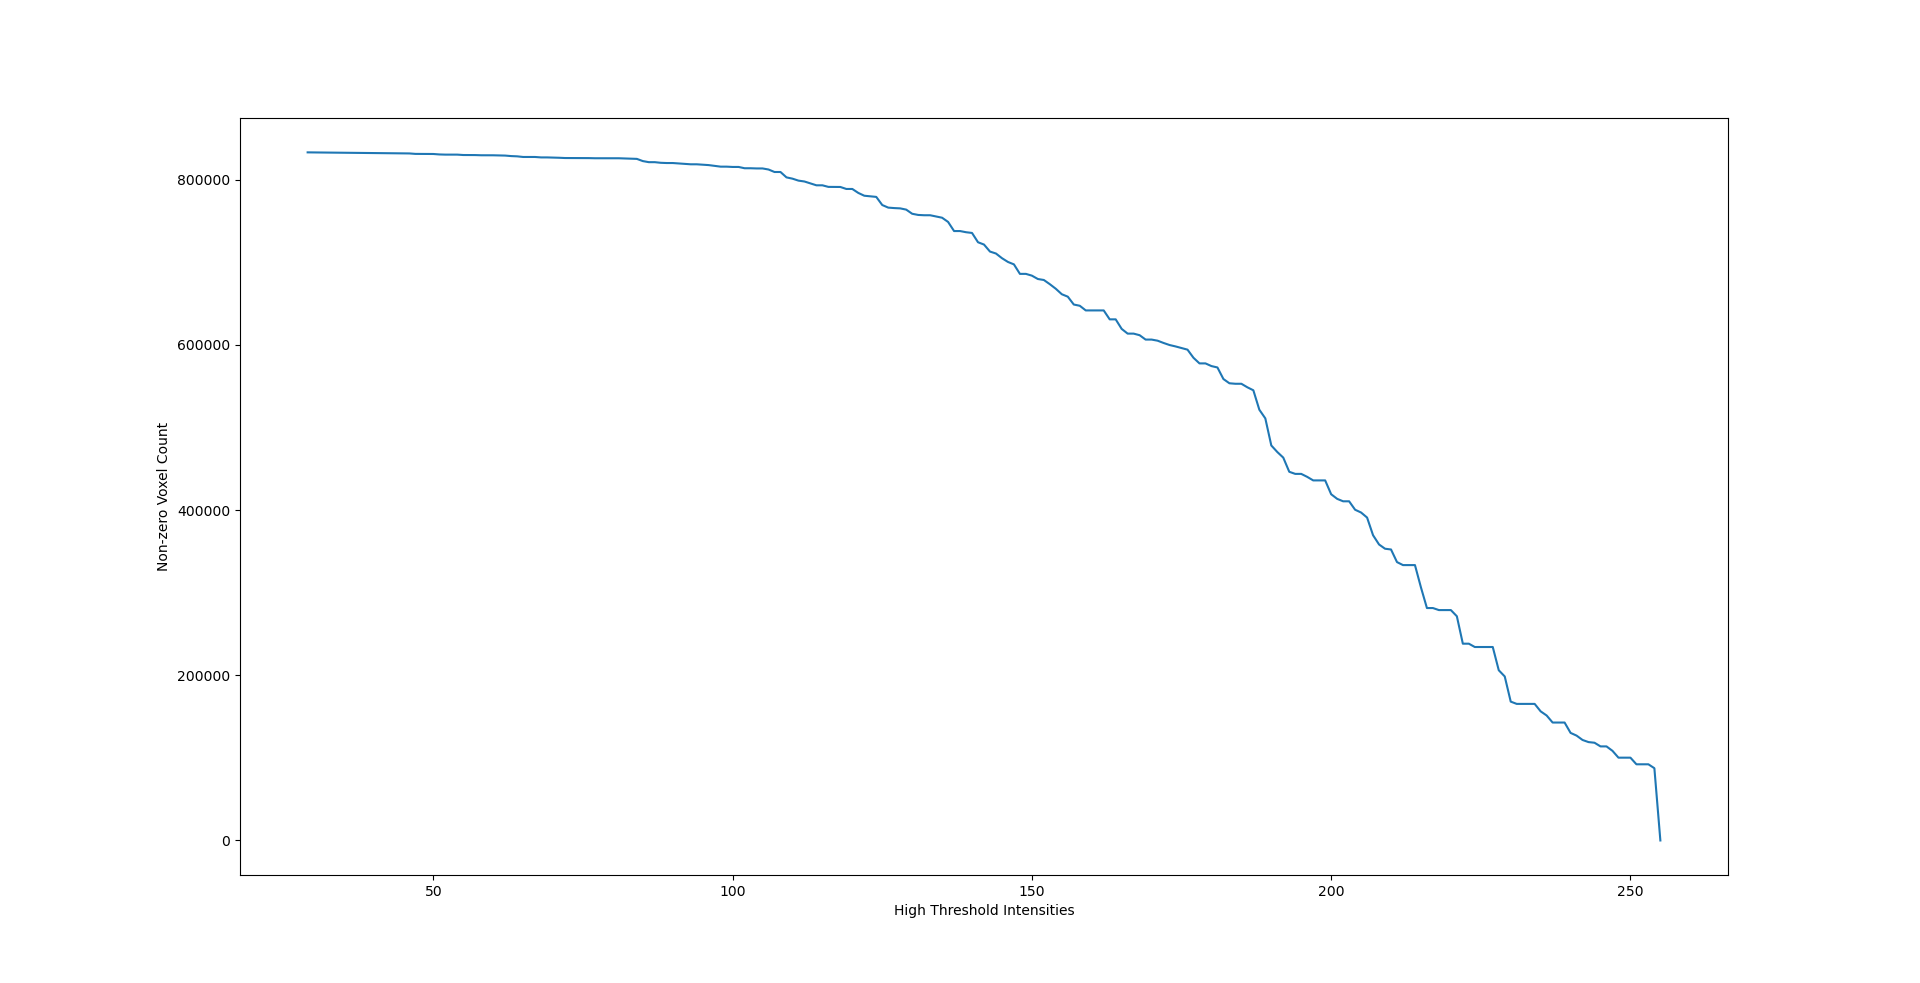
\includegraphics[width=0.49\textwidth]{figs/sample_ihh.png}}
    \caption[Examples of two opposing IHH's from images with good and bad foreground to background separability.]{Examples of two opposing IHH's from images with good and bad foreground to background separability.}
    \label{fig:ihh_contrast_compare}
\end{figure}

\subsubsection{Using the IHH}
While it was realized that the IHH captured information regarding the foreground and background separation of an image in a non-increasing distribution the challenge remained in reliably exposing features to quantify without muddling the understanding of what the distribution describes. After evaluating the IHH shape and its implications regarding the distribution of potential foreground over a range of high threshold strictness it was hypothesized that desired thresholds are likely to situate around ``flat'' regions of the IHH. The reason that ``flat'' IHH regions were of interest is based on what the IHH itself describes which is the distribution of the maximal intensity of each structure in the image (after low threshold application) with structures persisting at larger high thresholds being more within focus in the image. These flat regions were typically selected at lower high threshold intensities since we want to include as many potentially viable foreground structures in future analysis but this was based on an observation made with visual analysis. Regardless, this lead to the investigation of two fronts:
\begin{enumerate}
    \item Is a desirable threshold typically located on or adjacent to a relatively ``flat'' region of the IHH?
    \item How can this be quantified in a manner which can be fed into an algorithm?
\end{enumerate}
\textcolor{red}{Do you think I should include a few examples showing that the relatively flat regions of the IHH correlate with being near a threshold that would render a viable binarization outcome?}
With the objectives made clear experimentation began where the first objective was heuristically confirmed, although partially, that although there was no definitive proof there was a near pattern where `viable' high thresholds were situated near relatively flat IHH regions with a low margin of error. The real challenge came into the quantification of this with regard to detecting a `flat' region (how flat must it be for consideration?) and if there are multiple flat regions how should the selection be made between them?
\subsubsection{IHH gradient} 
The IHH gradient was believed to be the most effective solution to this where a gradient instead of a derivative would be used. The reason that either of these would be used is that if the slope of the IHH can be seen as representing the change in the IHH value then a flat IHH region would have no slope where the steepness of the slope is described by the gradient or the derivative. The gradient is what was decided to be used as the derivative requires some generalization of the IHH distribution function but said function cannot be inferred from the IHH thus the gradient evaluated against the distribution itself is more viable where the change in the IHH magnitudes ($y(n)$) between sequentially increasing intensity values ($x(n)$) can be measured as shown in Equation \ref{eq:slope_eq}. An illustration of an IHH and the gradient representation ($y'(n)$) can be seen in Figure \ref{fig:ihh_grad_compare}.
\begin{equation}\label{eq:slope_eq}
    m(n) = \lvert\frac{\Delta y(n)}{\Delta x(n)}\rvert = \lvert\frac{y(n)-y(n-1)}{x(n)-x(n-1)}\rvert\text{ where $N\geq n\geq 1$}
\end{equation}
\textcolor{red}{I am also considering having a figure where I highlight a region of the gradient representation with a high magnitude and match it to the same intensity window in the normal IHH and then colour code an MIP accordingly. The colouration in both graphs will be based on the intensity (the high threshold value that the pop out after) and this colouring will be mapped to the MIP with all other structures remaining grayscale. This would illustrate how an intensity range in flux could be composed of uncertainty. The same could be done with flat regions. Let me know your thoughts.}
\begin{figure}
    \centering
    \subcaptionbox{The original image IHH\label{subfig:original_ihh}}{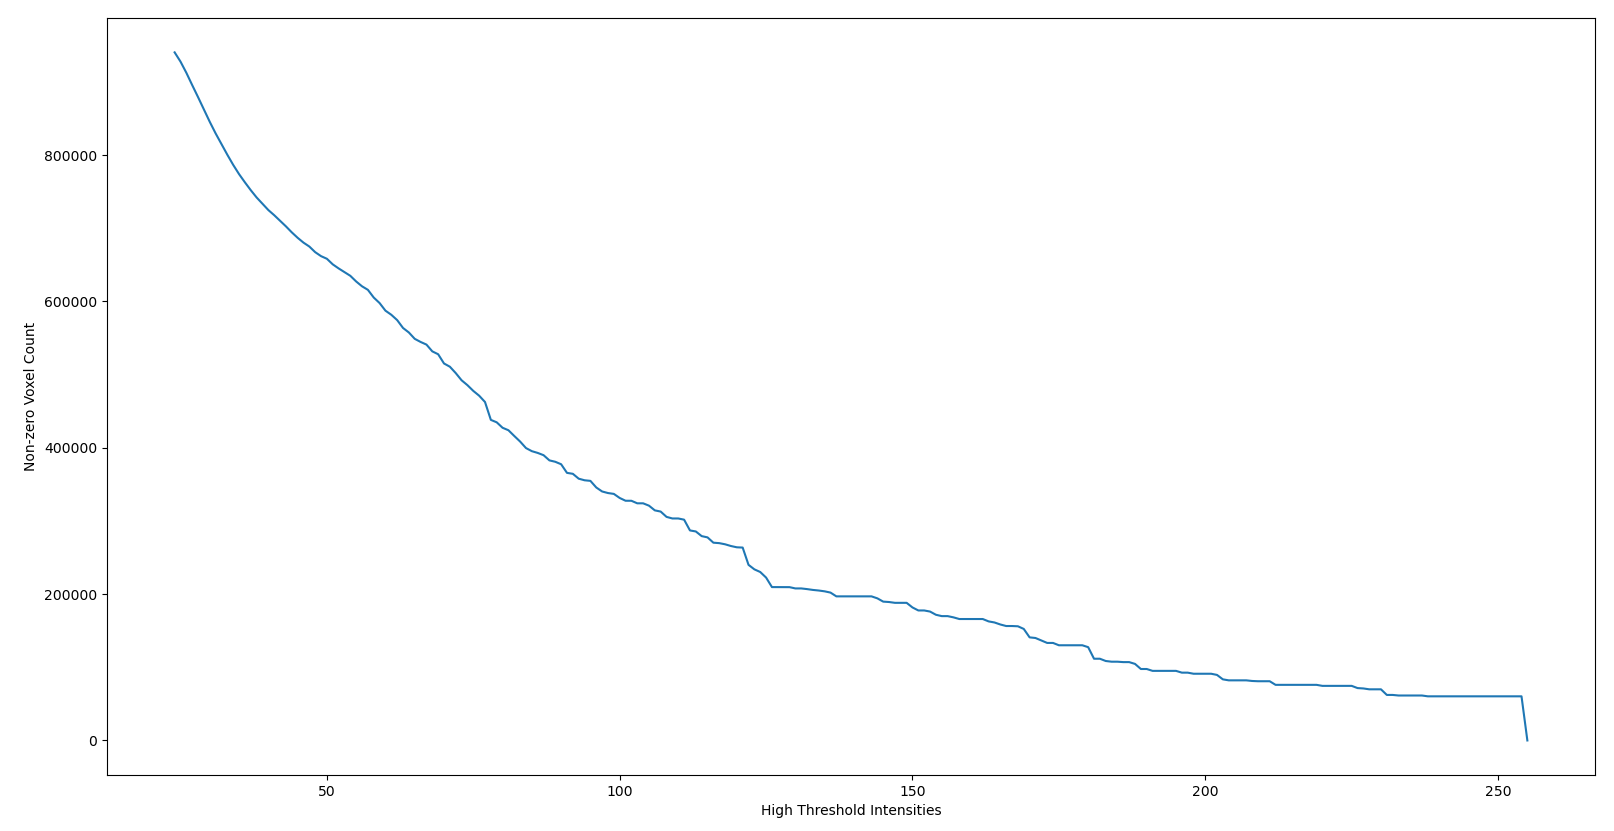
\includegraphics[width=0.48\textwidth]{figs/sample_ihh_bad.png}}
    \subcaptionbox{The gradient representation of \subref{subfig:original_ihh})\label{subfig:discrete_grad}}{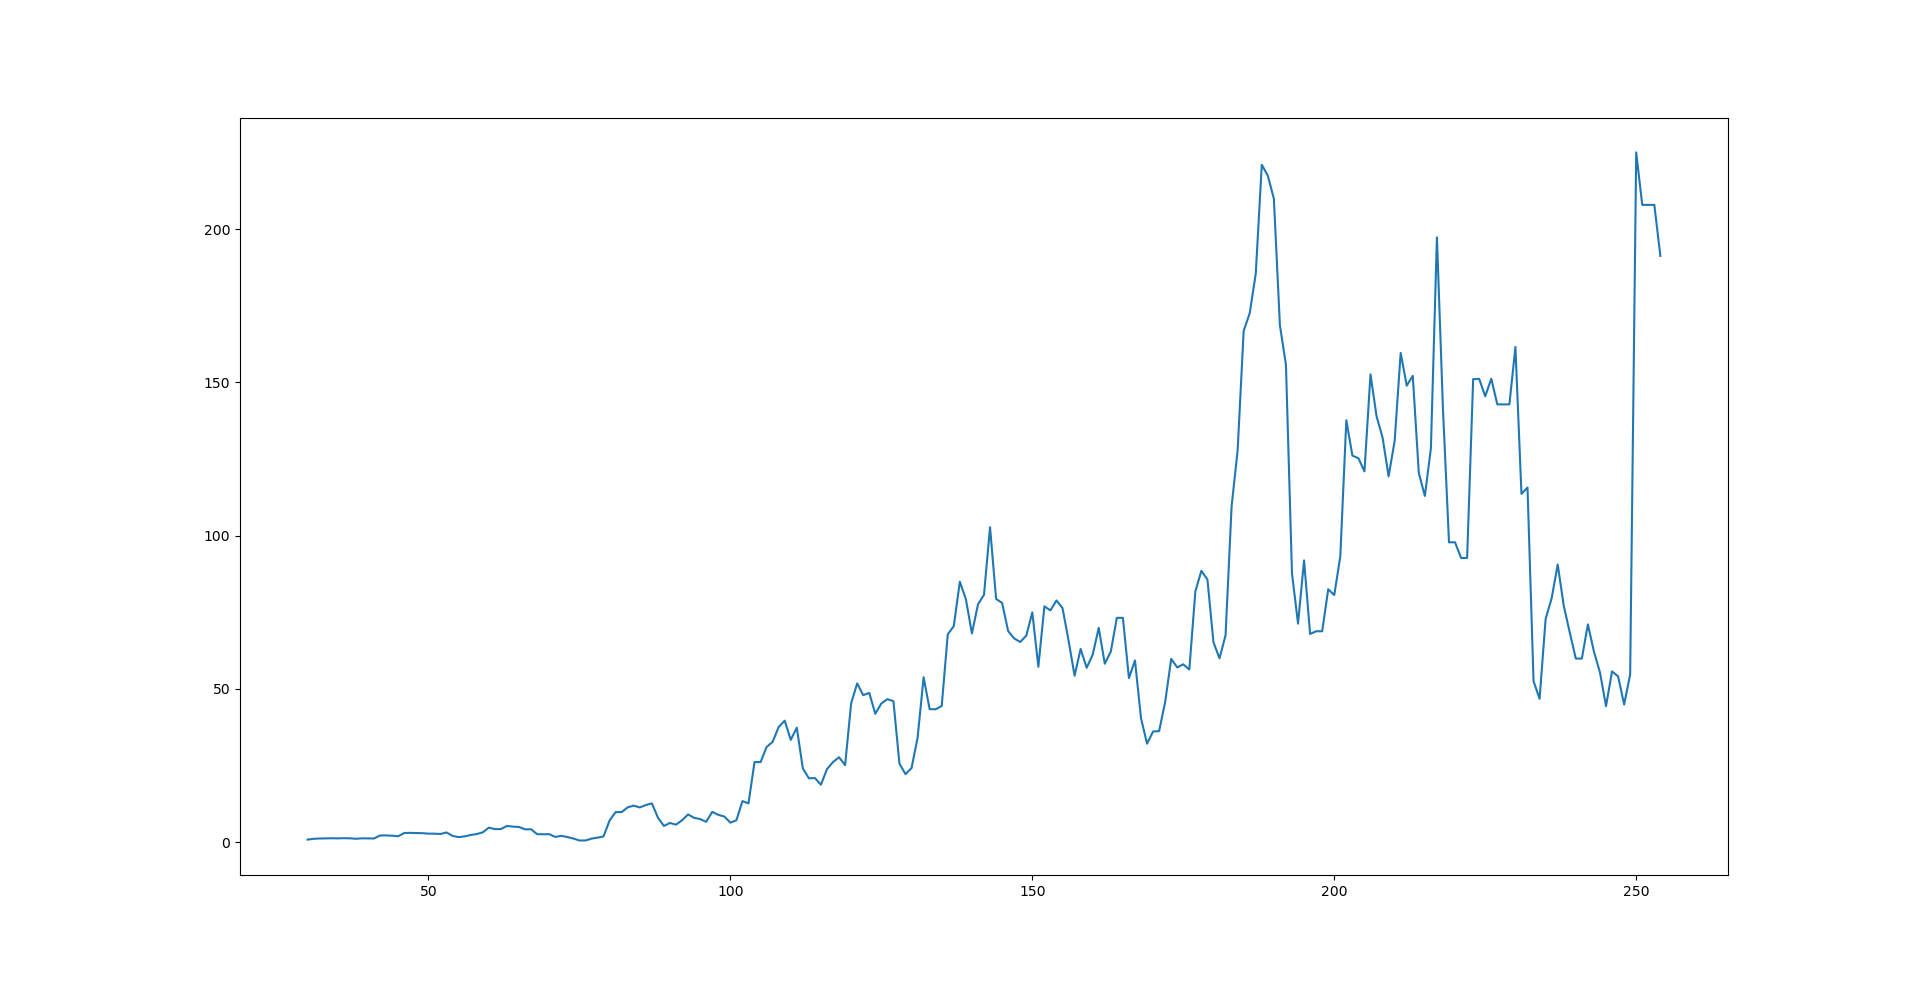
\includegraphics[width=0.48\textwidth]{figs/norm_ihh_slopes.png}}
    \caption[Comparison between the original IHH representation and the IHH gradient of Figure \ref{subfig:mip_bad_contrast_ihh}]{Comparison between the original IHH \textbf{(\subref{subfig:original_ihh})} representation and the IHH gradient \textbf{(\subref{subfig:discrete_grad})} of Figure \ref{subfig:mip_bad_contrast_ihh}}
    \label{fig:ihh_grad_compare}
\end{figure}
\paragraph{The problem} is that the gradient that we calculated does express the change in total structure volumes at increasing high threshold strictness but it is quite discrete as it only measures this change between consecutive intensities and it cannot capture changes expressed across an extended range of intensities and it is not uncommon for trends to be expressed over a range of values based on the shape of the IHH. A second problem found from this is that the resulting gradient distribution can have a noisy appearance due to the discrete approach used to calculate the gradient representation, as can be seen in Figure \ref{subfig:discrete_grad},  which increases the difficulty in numerically evaluating trends in the distribution to estimate where might be a potential point for high threshold selection. An example of this would be if, hypothetically, the ideal point is the minimum value within the distribution or some minima going from the lowest point of the high threshold range to the maximum. It could be caught in a sub-optimal local minima. These examples are stated while ignoring the potential challenges or problems those methods raise but regardless this noisy representation obscures the trends in the gradient representation that actually describe the high threshold strictness (or sensitivity) behaviour for an image and how the overall binarization responds to said behaviour.
\paragraph{The solution} proposed was to apply a smoothing operation using a rolling average where an intensity window (of size $W$) is designated and centred on a gradient representation magnitude $y'(n)$ at an intensity $n$. This centred window is then rolled across the full range of intensities $N$ where the average $\overline{y}'(n)$ is used as the new smoothed gradient value ($\overline{y}'(n)$ at $n$. This is seen in Equation \ref{eq:average_window} with $m_1$ and $m_2$ being the bounded upper and lower window ranges as described in Equation \ref{eq:av_win_conditions} where $m_1$ and $m_2$ are both $W/2$ save for when the centre of the window ($n$) is too close to the bottom ($n\to 0$) or end ($n\to N$) of the range. When the centre is too close the lower ($m_1$) or upper ($m_2$) bound of the window is shortened to fit in the reduced range and so too is the length of the window by which the value is divided by, given that the window contains less values to average.
\begin{align}\label{eq:average_window}
        \overline{y}'(n) &= \frac{\sum_{t=n-m_1}^{n+m_2}y'(t)}{m_1+m_2}\\ \label{eq:av_win_conditions}
    \text{ where }m_1 &=\begin{cases}
        0, & \text{if } n=0\\
        \leq W/2, & \text{if } n \leq W/2\\
        w/2, & \text{if } n \geq W/2
    \end{cases}
    \text{and }m_2 = \begin{cases}
                0, & \text{if } n=N\\
        \leq W/2, & \text{if } n \geq N-W/2\\
        w/2, & \text{if } n \leq N-W/2
    \end{cases}
\end{align}
\textcolor{red}{Here I state that the window size will be 8 for use in the system development. Should I in Chapter 4 briefly explore the impact of the window size on the system results or should I append that to this subsection or chapter?}
Through heuristic testing, a window size of $8$ was decided for use as it did not overly smooth the distribution via diminishing the trends but noisy behaviours were sufficiently suppressed. This was evaluated by visual analysis of the smoothed gradient representation of the IHH were it was observed that a smoothing window of $8$ functioned optimally for a subset of samples but further testing will be performed accompanied by numerical evaluations of the impact on performance the window size has. 

\subsubsection{IHH gradient inversion}
With the discrete noisy behaviour smoothed down while preserving the trends, a method to identify ideal regions was still required although the basis that flat IHH regions will inform this was still maintained. As comparatively flatter regions of the gradient IHH contribute more weight to the high threshold selection an inversion of the gradient representation magnitude is performed such that the values used in the distribution better reflect the intended use of them in further algorithms. There were two methods by which the representation was to be inverted with the first being a sigmoid-based approach while the latter was a linear inversion. This sigmoid-based approach would employ the use of the logistic function to invert the smoothed gradient distribution to invert and scale the weight contributions of flatter regions. The motivations around this were initially that the occurrence of completely ``flat'' regions in the gradient distribution was ideal but also naive and there was no certainty that it would be present within any of the distributions. Due to this flatness limitation, a softer inversion method using the logistic function that could be tuned was first approached. This application projected the gradient representation magnitudes ($y$-axis) along the logistic function dependent variable ($x$-axis) with the resulting new magnitudes being based on the steepness parameter of the logistic function. What is consistent is that the lowest gradient magnitude will become $1$ after re-weighting while the maximum gradient magnitude will become $0$ but a steepness parameter with a resulting \textit{S}-shaped curve, as shown in Figure \ref{fig:logistic_rescaling}, will result in a clustering of $n$ of the bottom and top of the gradient magnitude. This results in a new distribution that essentially states ``values close to the peak are essentially all experiencing too much change while values within a low enough margin of magnitude of change are approximately the same'' reducing nuance but also emphasizing broad trends of the extreme gradient representation values. 
\begin{figure}
    \centering
    \subcaptionbox{Logistic inversion function with low steepness \label{subfig:low_steep_logist}}{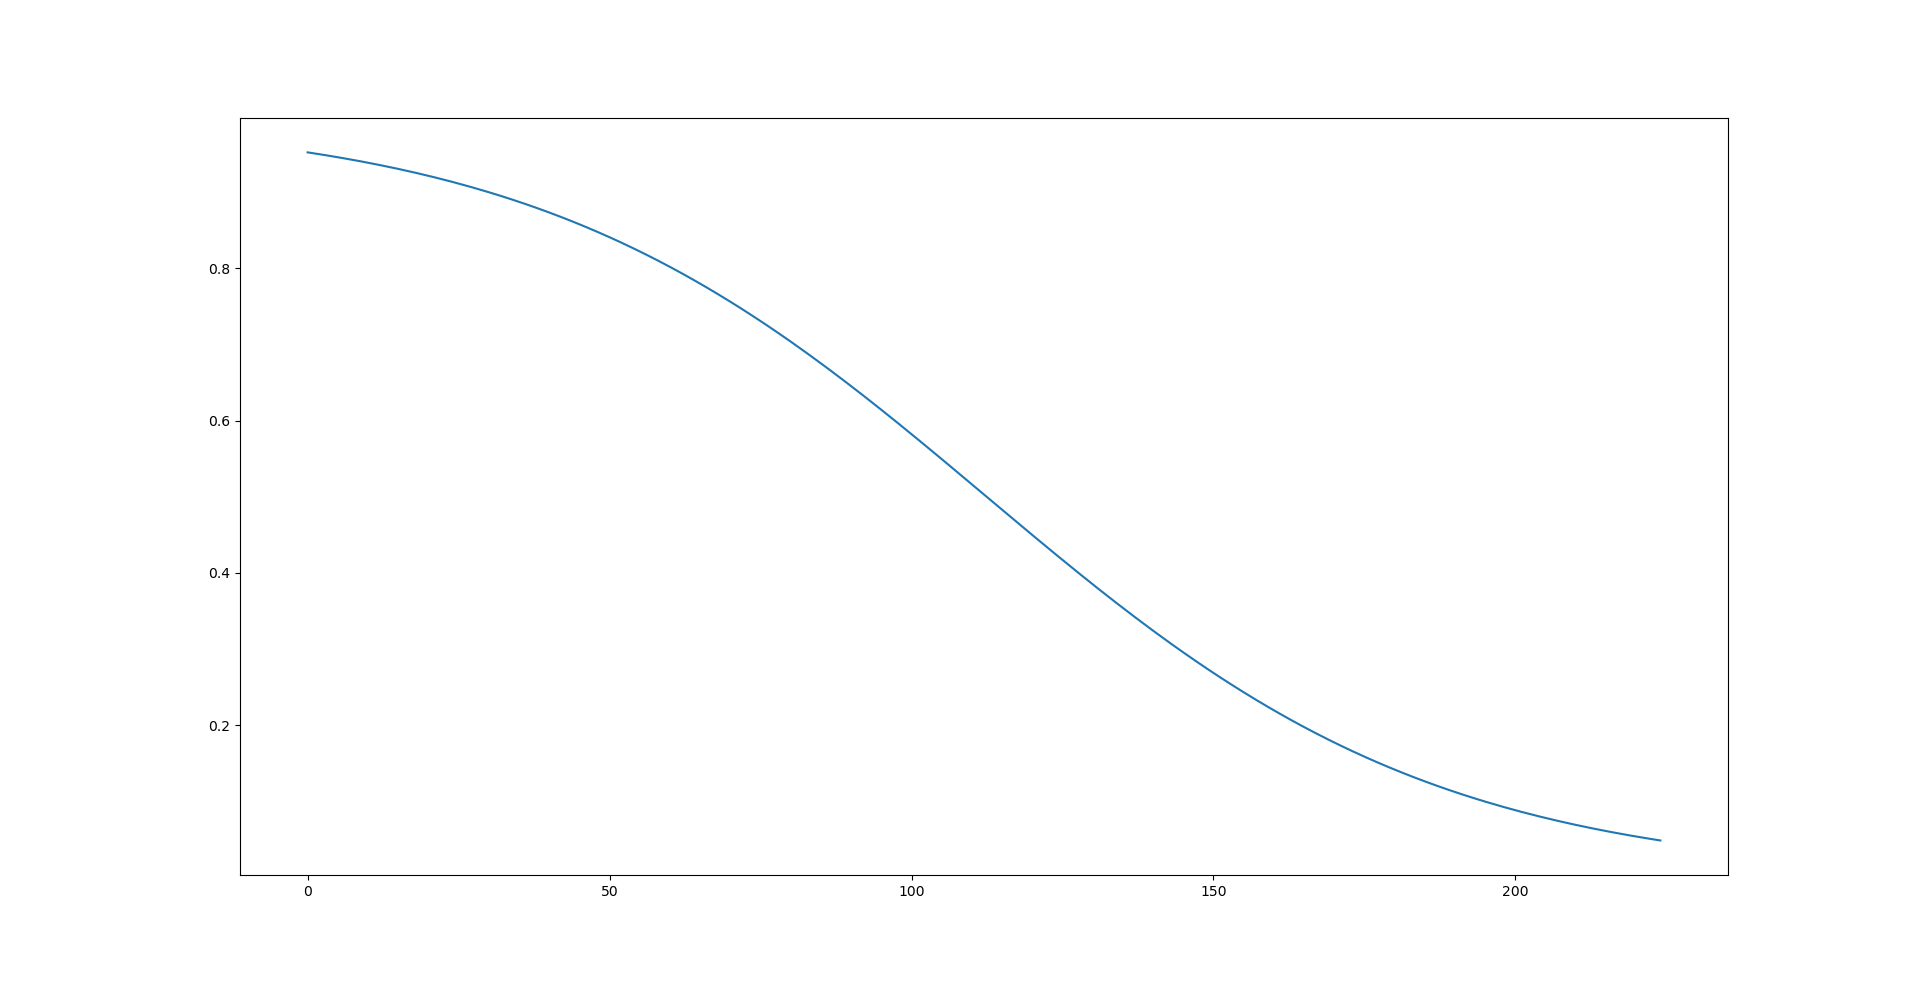
\includegraphics[width=0.49\textwidth]{figs/Rescale_dist_6.png}}
    \hfill
    \subcaptionbox{Logistic inversion function with high steepness\label{subfig:high_steep_logist}}{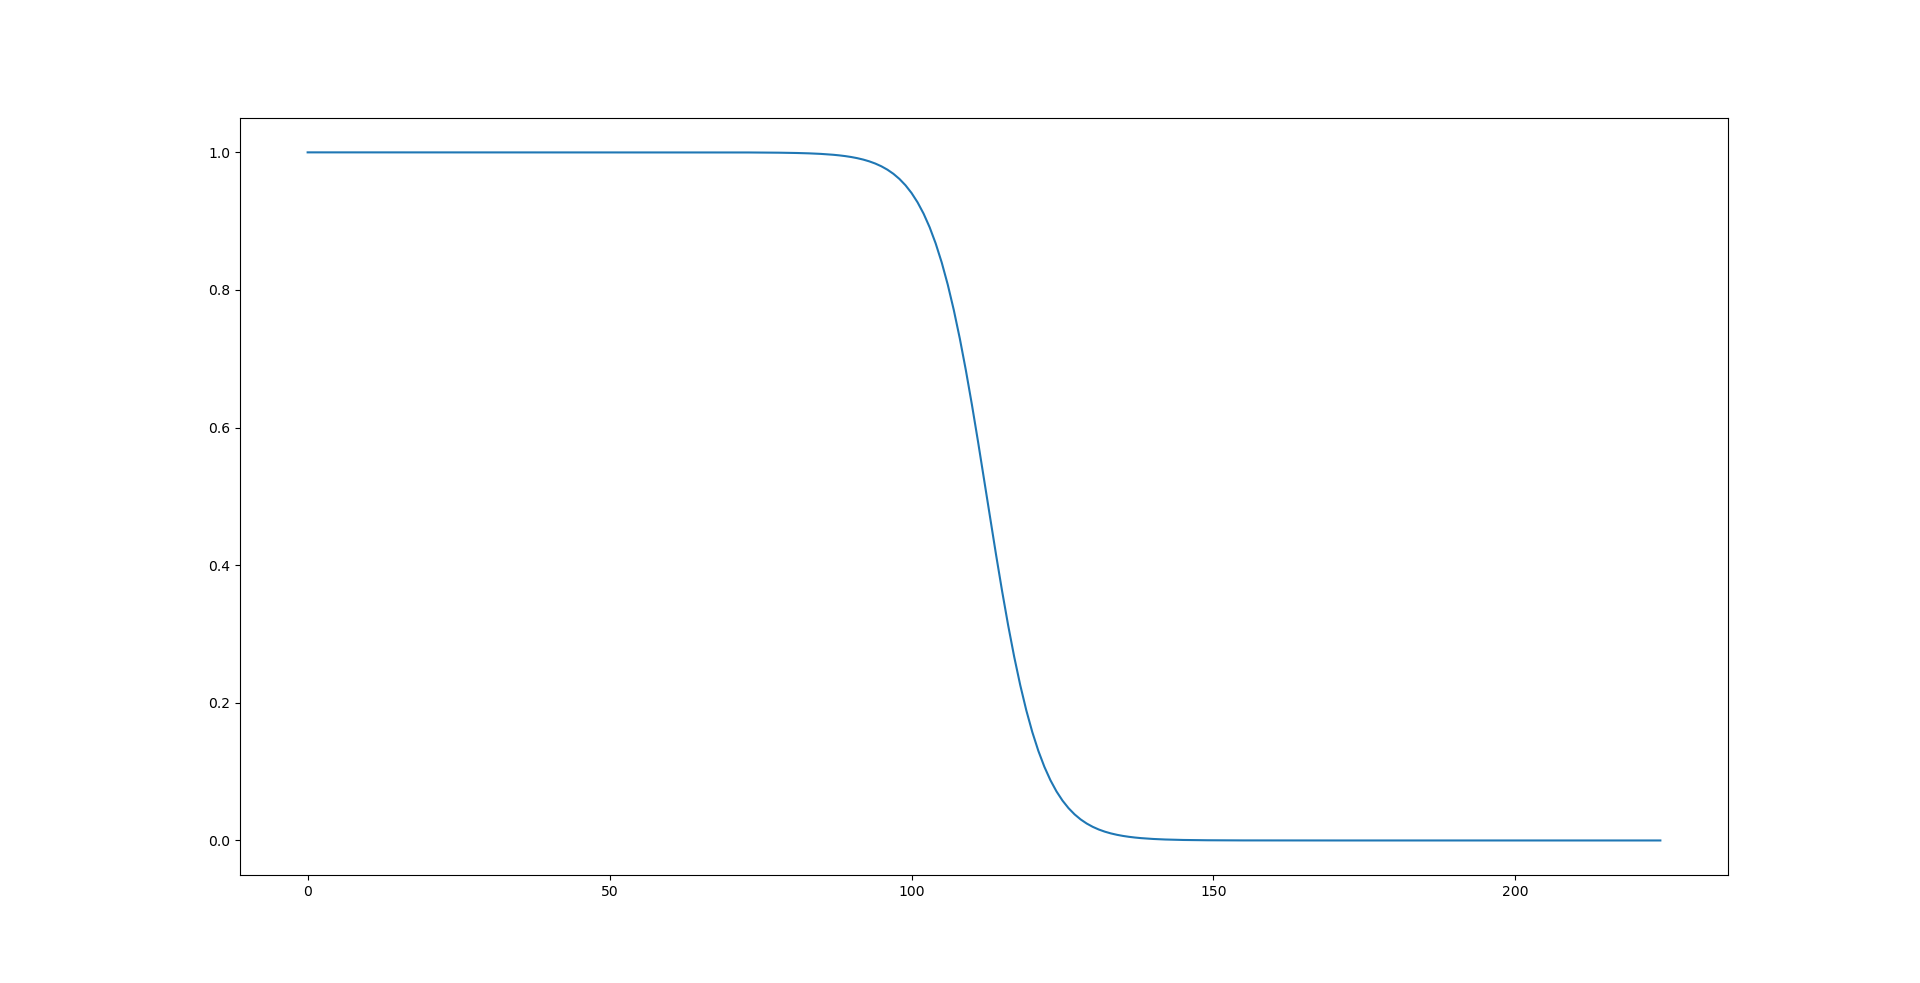
\includegraphics[width=0.49\textwidth]{figs/Rescale_dist_50.png}}
    \subcaptionbox{Resultant Inversion using a low steepness logistic function\label{subfig:low_steep_invert}}{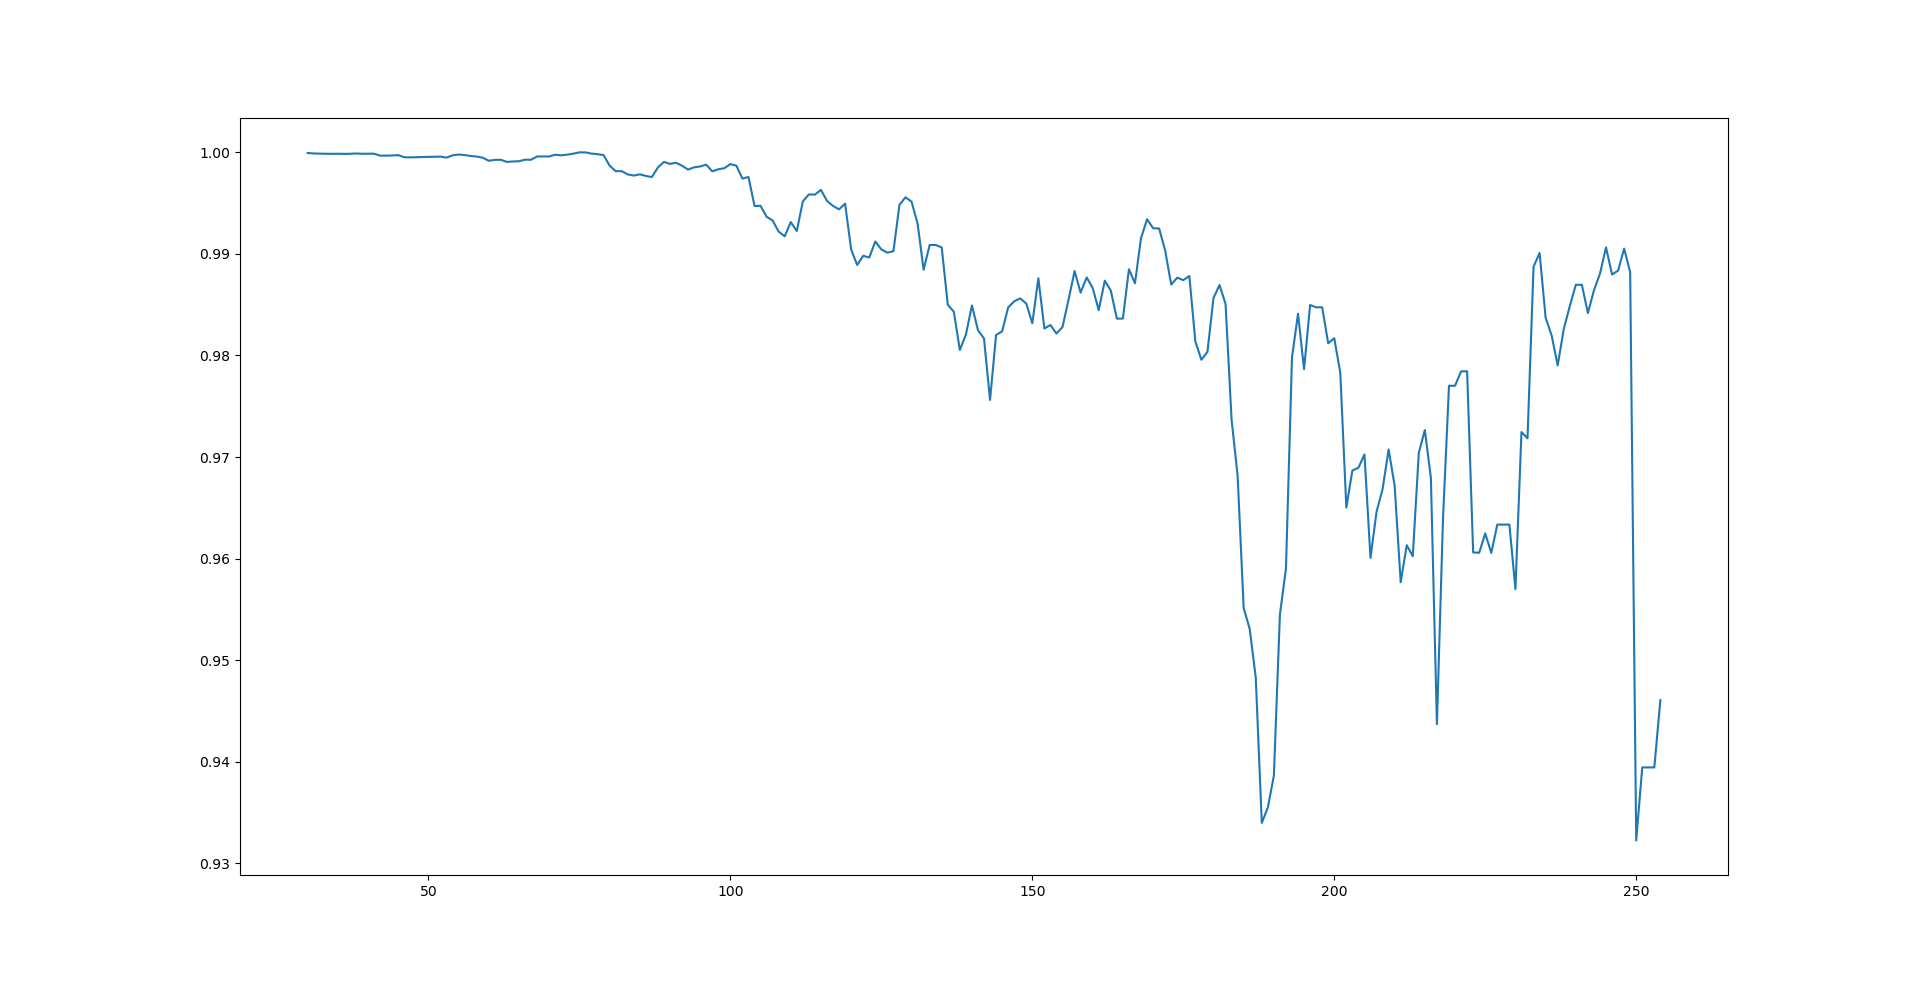
\includegraphics[width=0.49\textwidth]{figs/Logist_rescale_slope.png}}
    \hfill
    \subcaptionbox{Resultant Inversion using a high steepness logistic function \label{subfig:high_steep_invert}}{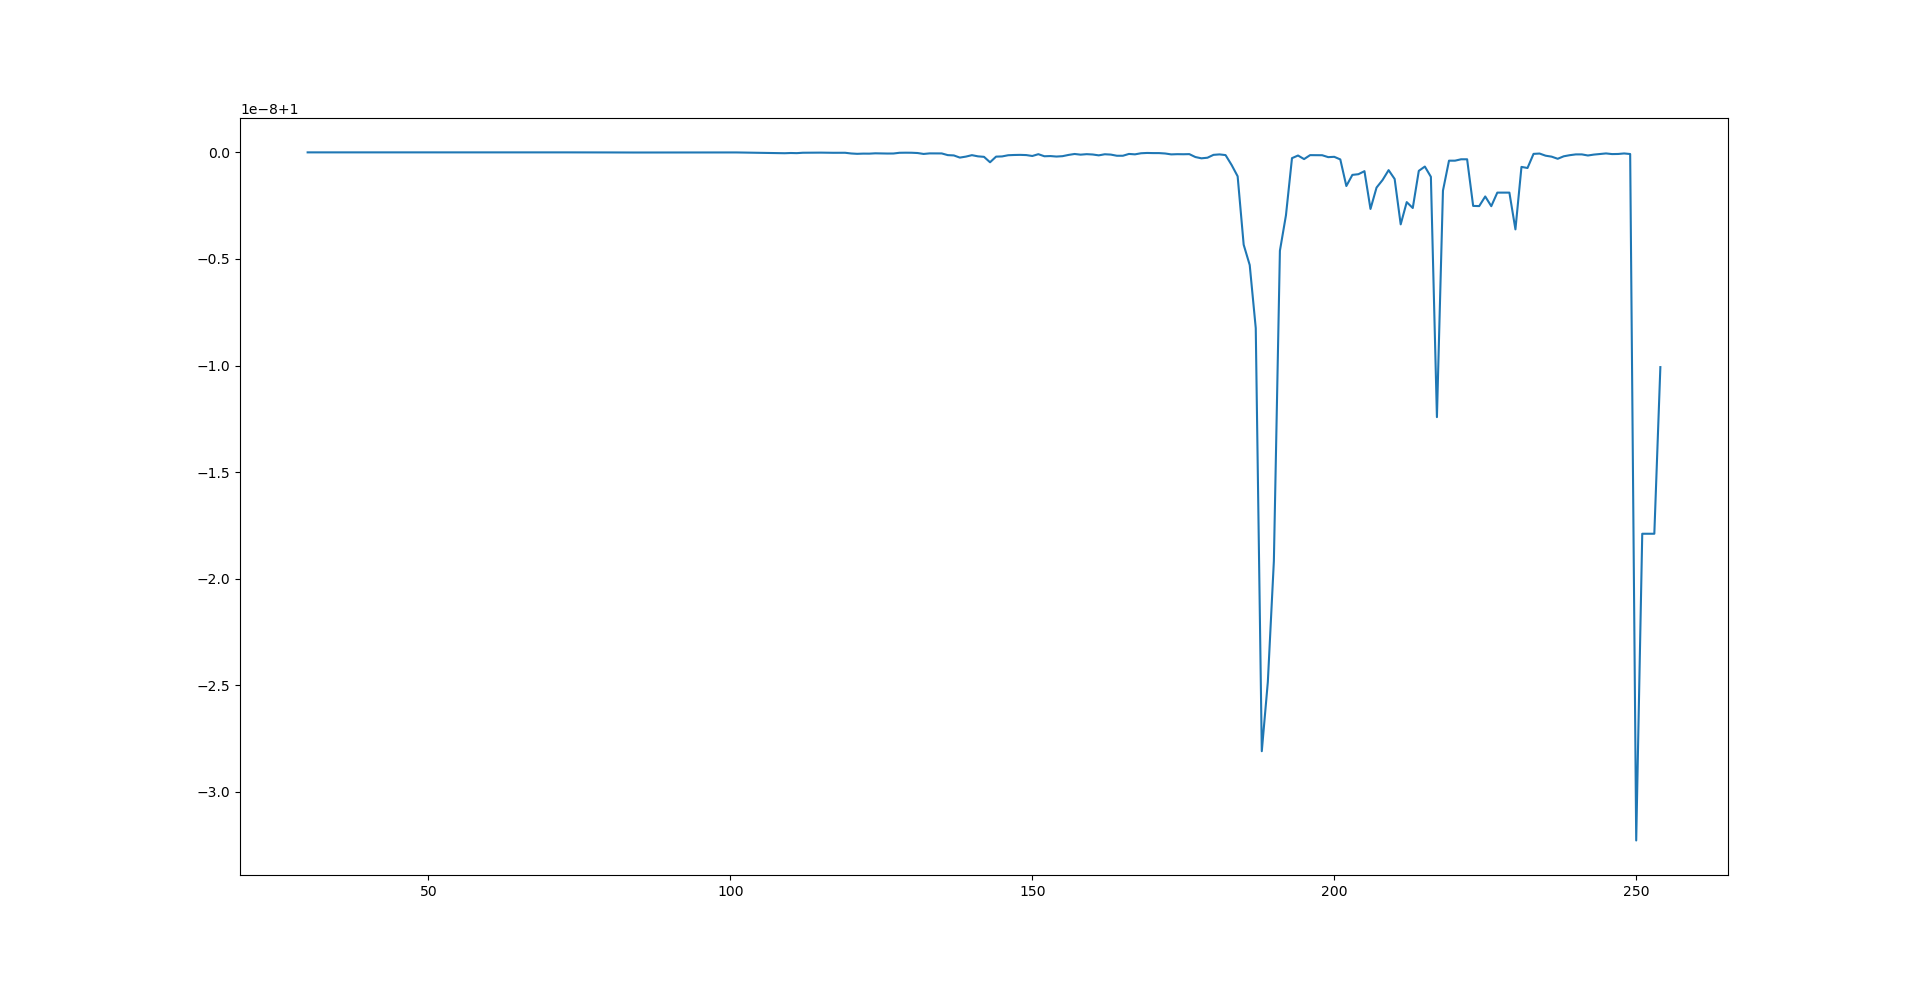
\includegraphics[width=0.49\textwidth]{figs/Logist_rescale_slope_50.png}}
    \subcaptionbox{Original smoothed Gradient IHH with the projected logistic function (low steepness) parallel to the $y$-axis and the resulting inversion parallel to the $x$-axis \label{subfig:low_steep_joint}}{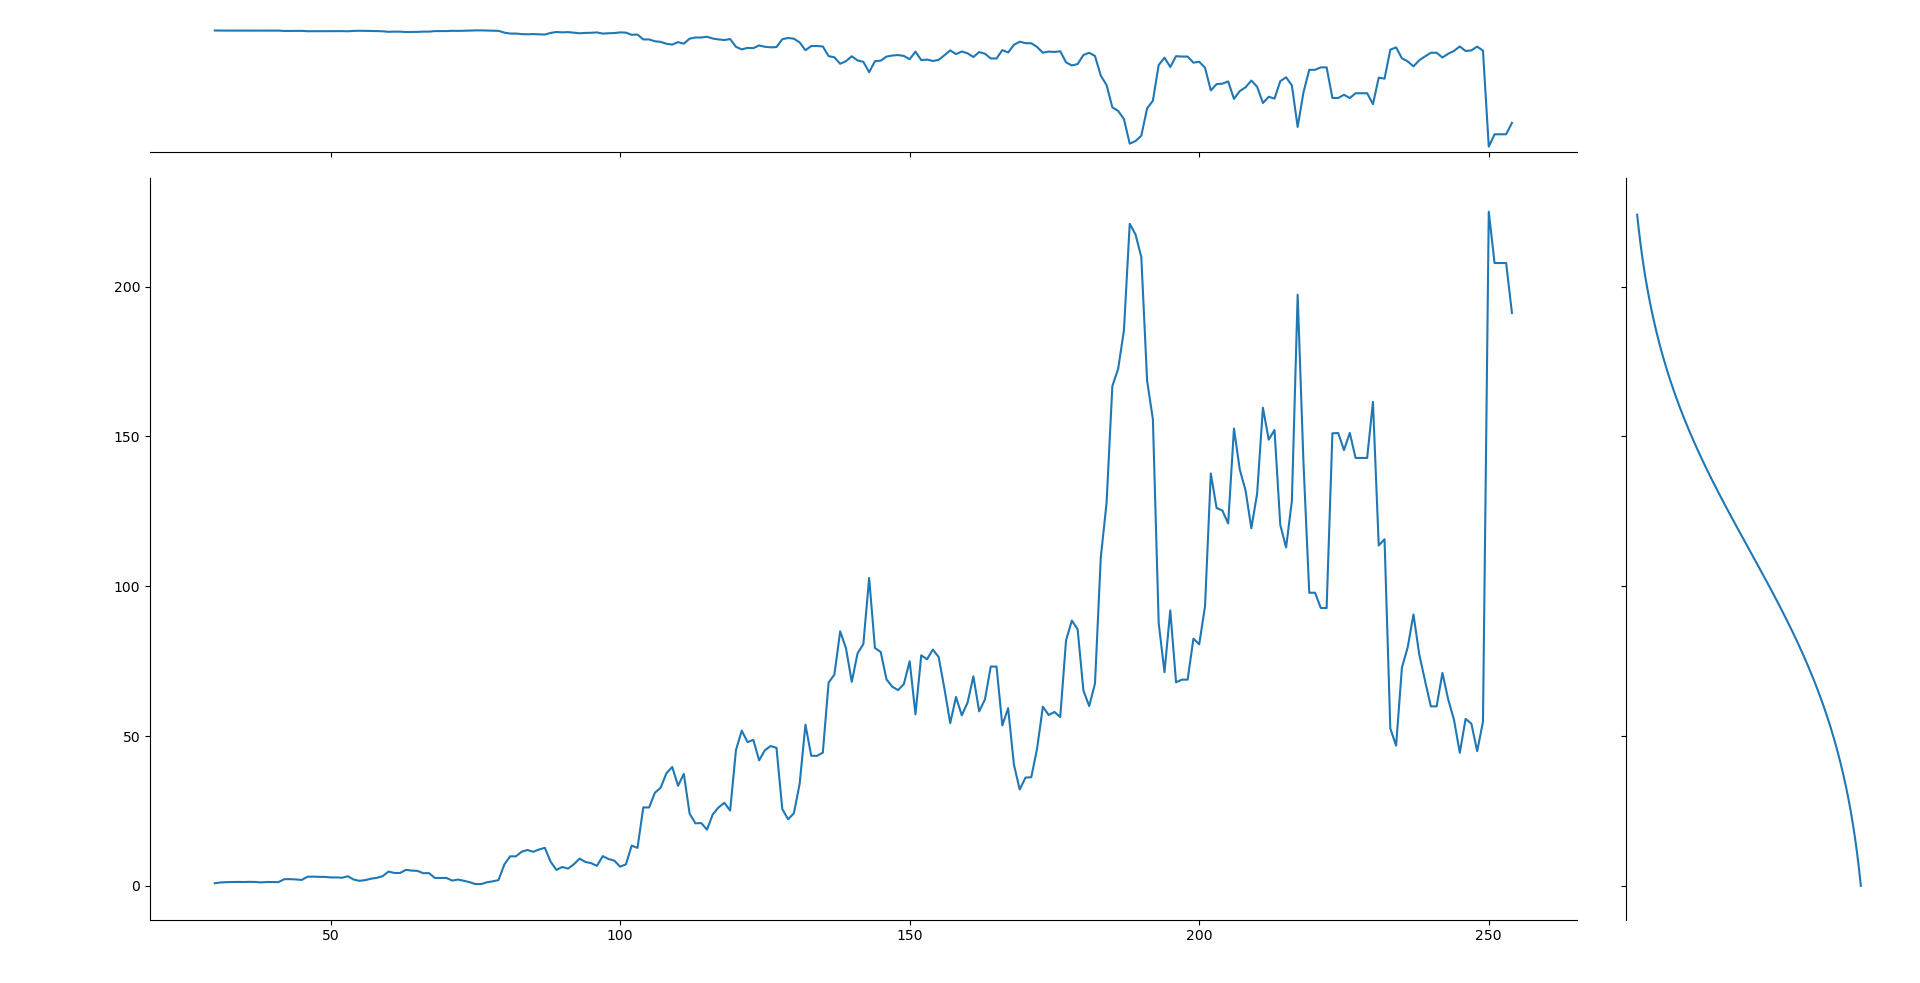
\includegraphics[width=0.49\textwidth]{figs/Joint_rescale_ihh.png}}
    \hfill
    \subcaptionbox{Original smoothed Gradient IHH with the projected logistic function (high steepness) parallel to the $y$-axis and the resulting inversion parallel to the $x$-axis \label{subfig:high_steep_joint}}{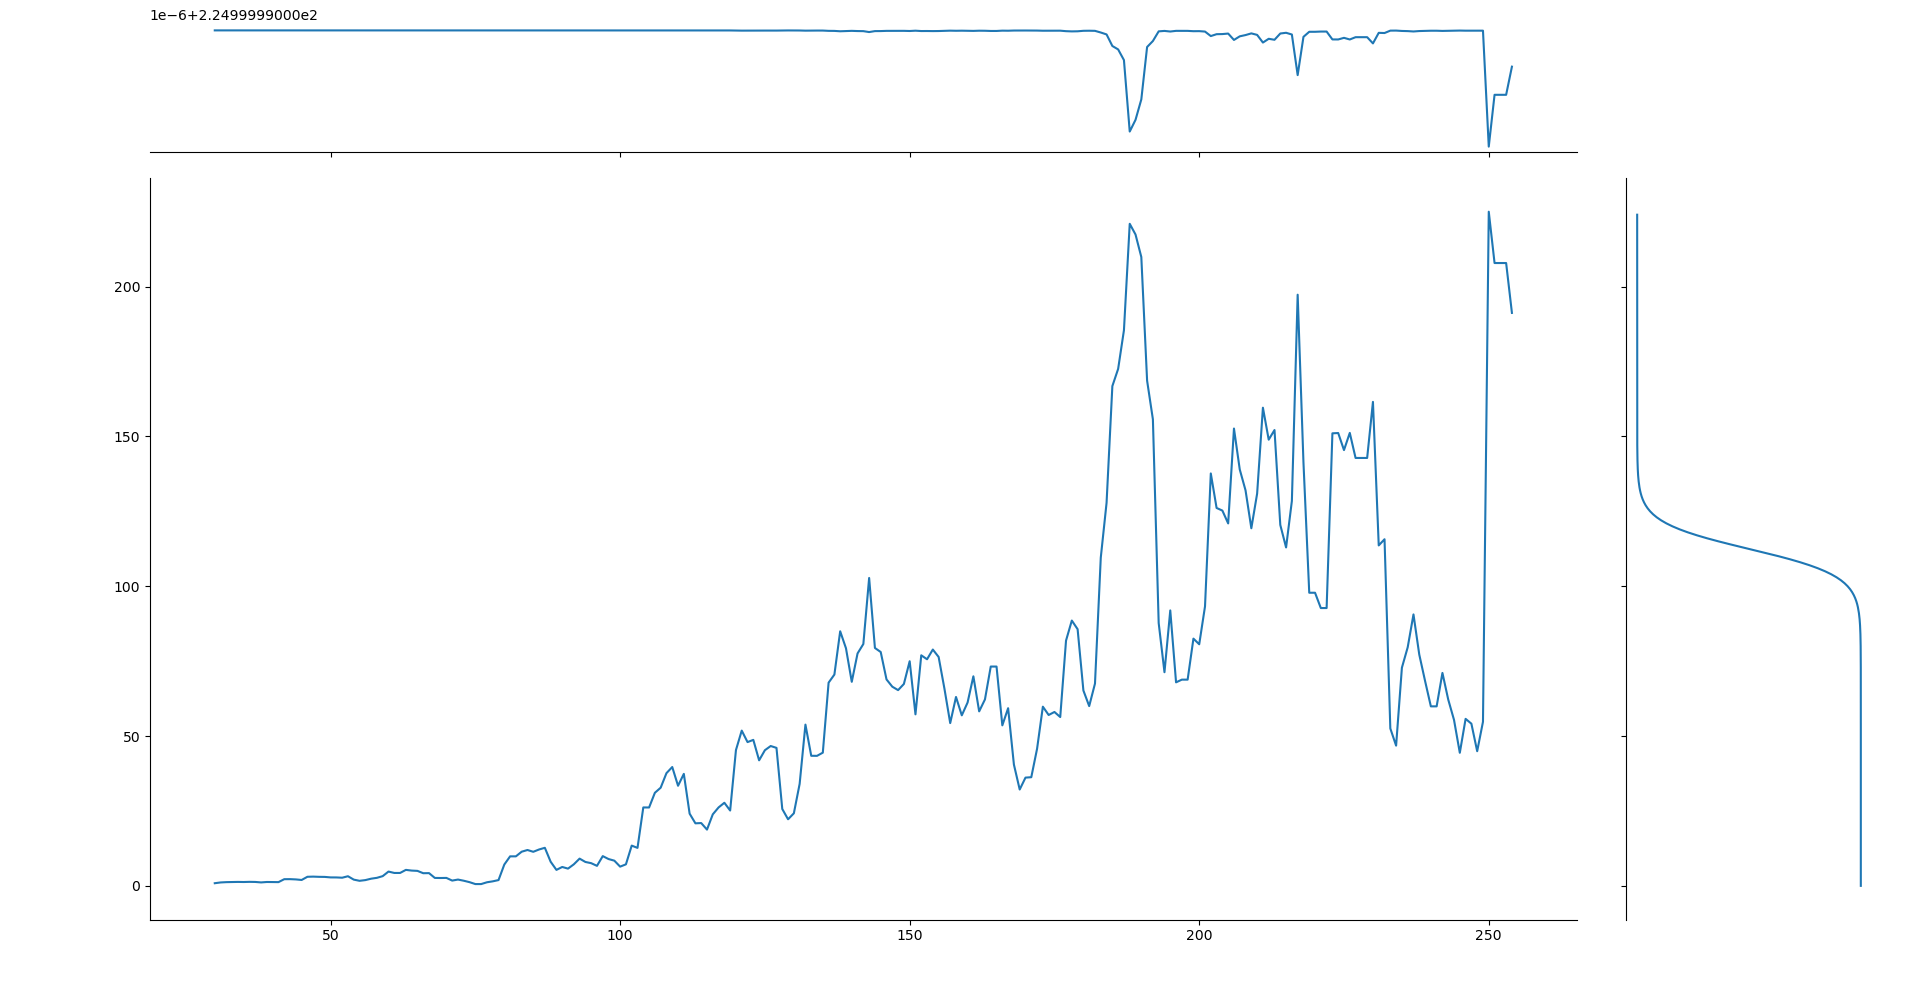
\includegraphics[width=0.49\textwidth]{figs/Joint_rescale_ihh_50.png}}
    \caption[Logistic function projection of smoothed gradient representation magnitudes with resulting re-weighting]{Logistic function projection of smoothed gradient representation magnitudes with resulting re-weighting. The original IHH can be seen in Figure \ref{subfig:discrete_grad} with the logistic function to invert it shown in figures (\subref{subfig:low_steep_logist}) and (\subref{subfig:high_steep_logist}). The resultant inversion is shown in figures (\subref{subfig:low_steep_invert}) and (\subref{subfig:high_steep_invert}). A final representation is shown in Figures (\subref{subfig:low_steep_joint}) and (\subref{subfig:high_steep_joint})
    }
    \label{fig:logistic_rescaling}
\end{figure}
This introduced a new tunable parameter and although a value of $6$ was settled on, for the purposes of developing subsequent features, further rigorous testing would be required to fully discern the impact of the logistic function shape, based on the steepness parameter, on the behaviour of the high threshold determination. Due to this, a more clear linear inversion was introduced in Equation \ref{eq:linear_inv} where the magnitudes of the smoothed gradient distribution ($\overline{y}'(n)$) are subtracted from and divided by the maximum of the distribution ($\overline{Y}'_{\text{maximum}}$) for all intensity values ($n$) resulting in a normalized and flipped smoothed gradient distribution ( $\overline{y}'_{\text{new}}(n)$ ). The benefit of this is that the inversion will perform relatively consistently for gradient distributions regardless of the source image and that there will be no added tunable parameters while still achieving the desired outcome of emphasizing lower values in smoothed gradient distribution numerically.
\begin{equation}\label{eq:linear_inv}
    \overline{y}'_{\text{new}}(n) = \frac{\overline{Y}'_{\text{maximum}} - \overline{y}'(n)}{\overline{Y}'_{\text{maximum}}}
\end{equation}

\subsection{Selecting a high threshold}\label{sec:centroid_calc}
With the smoothed gradient IHH distribution inverted such that values of lower change in IHH values are emphasized a high threshold value needs to be selected. The key challenge regarding high threshold selection using the gradient distribution is the criteria used to determine what region is best fit as there can be multiple regions of varied degrees of flatness in the IHH which are expressed in the gradient representation with the result needing to be a single value. There were many attempts to determine a value similar to a mean of the intensities based on the inverted gradient distribution as weights and after experimentation, a method to achieve this was produced as shown in Equation \ref{eq:first_centroid}. In this function, there are $N$ sequential intensity values $x(n)$ that make up the $x$-axis of the inverted gradient distribution with the inverted gradient values $\overline{y}'_{\text{new}}(n)$ is used to weight the intensity value for each corresponding intensity $n$ and averaged by the total count of values composing the distribution $x$-axis. 
\begin{equation}\label{eq:first_centroid}
    C = \frac{\sum_{0}^{N} \overline{y}'_{\text{new}}(n)\circ x(n)}{N}
\end{equation}
The result of this is a value that acts similar to a centre of mass ($C$) for an object given that the inverted gradient magnitudes represent the mass contributions of each intensity value in the distribution thus some `best fit' result is achieved that takes all values across the distribution into account. After it was confirmed that this resulted in an intensity value calculated based on the gradient magnitudes the spectral centroid was discovered. Due to the greater context of how the algorithm should behave, based on Eq. \ref{eq:first_centroid}, the centroid calculation was discovered where a crucial difference is that the value is divided by the sum of the inverted gradient weights across the intensity range ($\sum_{0}^{N}\overline{y}'_{\text{new}}(n)$) as seen in Equation \ref{eq:actual_centroid}. The added benefit of this approach is that the divisor is the sum of intensity weights ($\sum_{0}^{N}\overline{y}'_{\text{new}}(n)$) resulting in a more accurate intensity centroid ($C_x$) using a method that is more mathematically robust which is more applicable to this use case.
\begin{equation}\label{eq:actual_centroid}
    C_x = \frac{\sum_{0}^{N} \overline{y}'_{\text{new}}\circ x(n)}{\sum_{0}^{N}\overline{y}'_{\text{new}}(n)}
\end{equation}
This final intensity centroid considers the distribution of `flatness' throughout the IHH which is expressed as values tending towards $1$ in the inverted gradient representation magnitude and selects a best-fit value but it was found that at times that the higher contrast resulted in very flat high intensities that contained far less object information than desired and the general approach is that if the system outcome is going to err then rather it err more lenient and preserve more voxels as foreground as these can be addressed with further processing but any voxels labelled as background may be wholly excluded from any further processing or evaluation risking information being lost.
\begin{figure}
    \centering
    \subcaptionbox{Distribution showing the inverted gradient representation with the two centroid outcomes annotated by vertical, dashed lines}{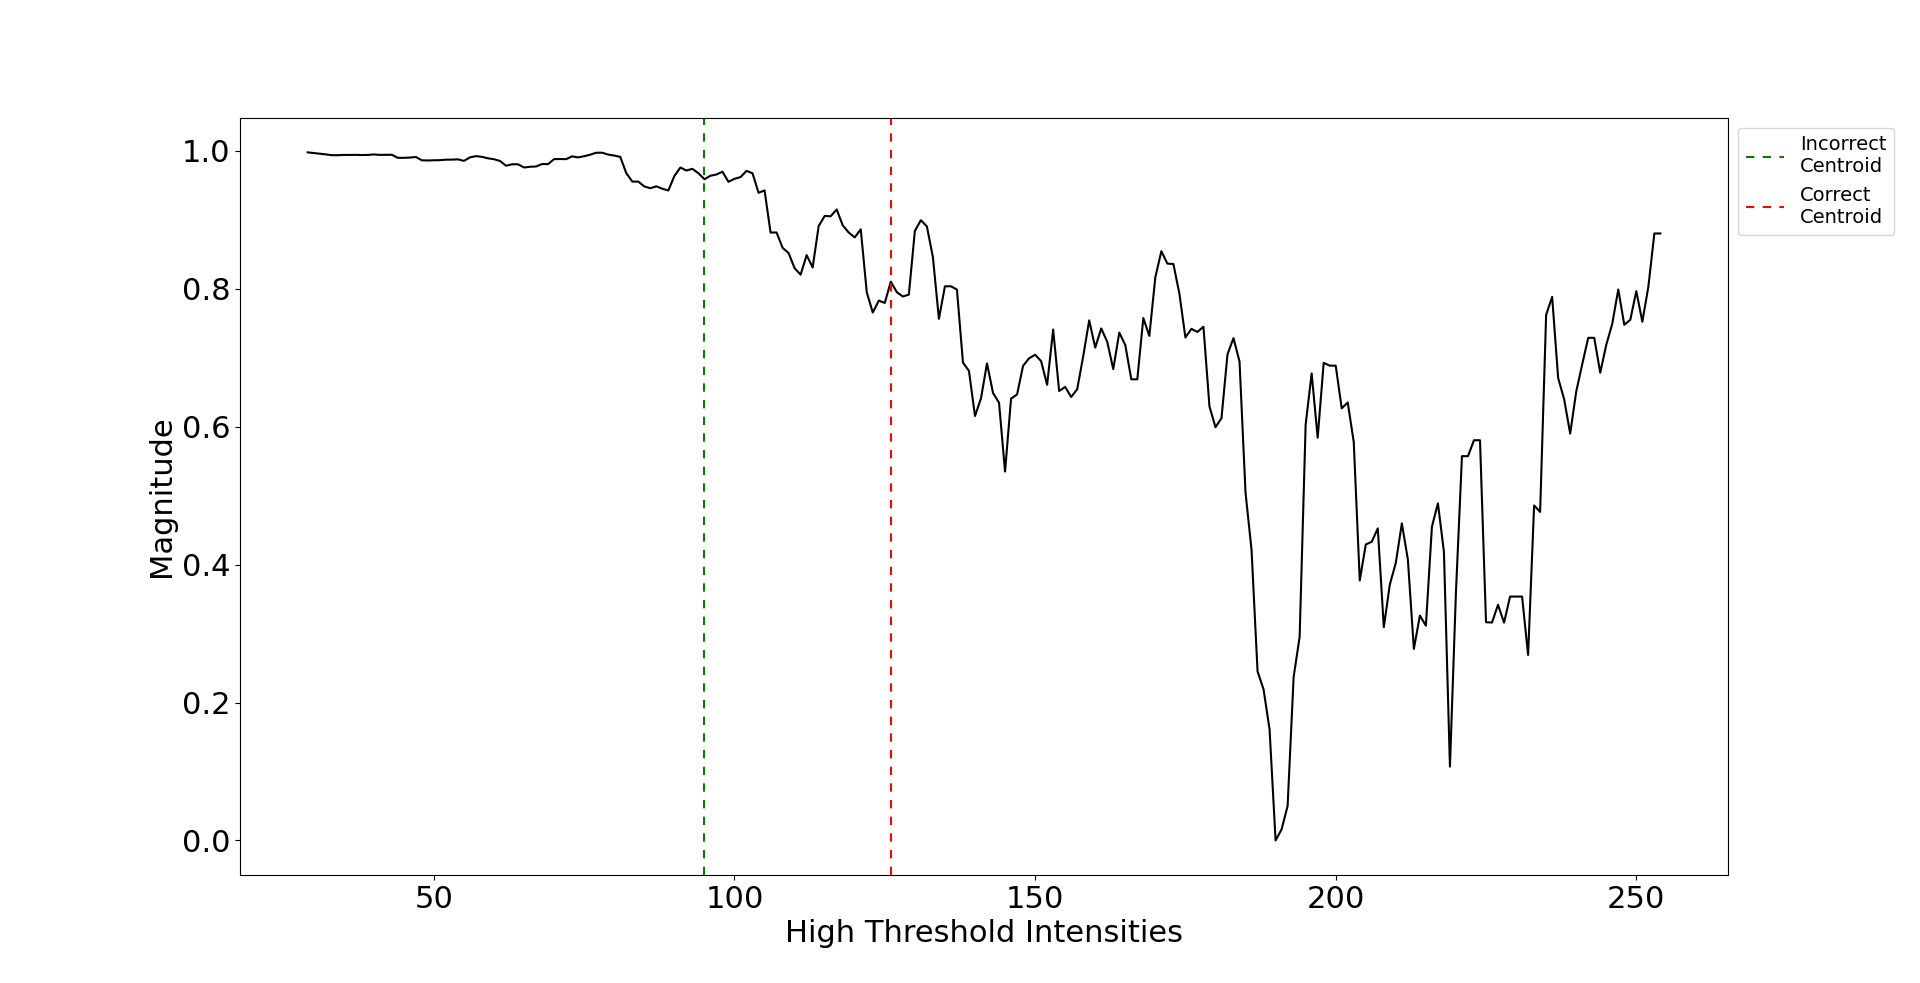
\includegraphics[width=0.59\textwidth]{figs/ch3figs/centroid_correction.png}}
    \subcaptionbox{The effect of these outcomes on the image thresholding. Blue describes the voxels above the low threshold; green describes all structures containing a voxel intensity above the incorrect centroid (\ref{eq:first_centroid}); and red describes all structures containing a voxel intensity above the correct centroid (\ref{eq:actual_centroid})}{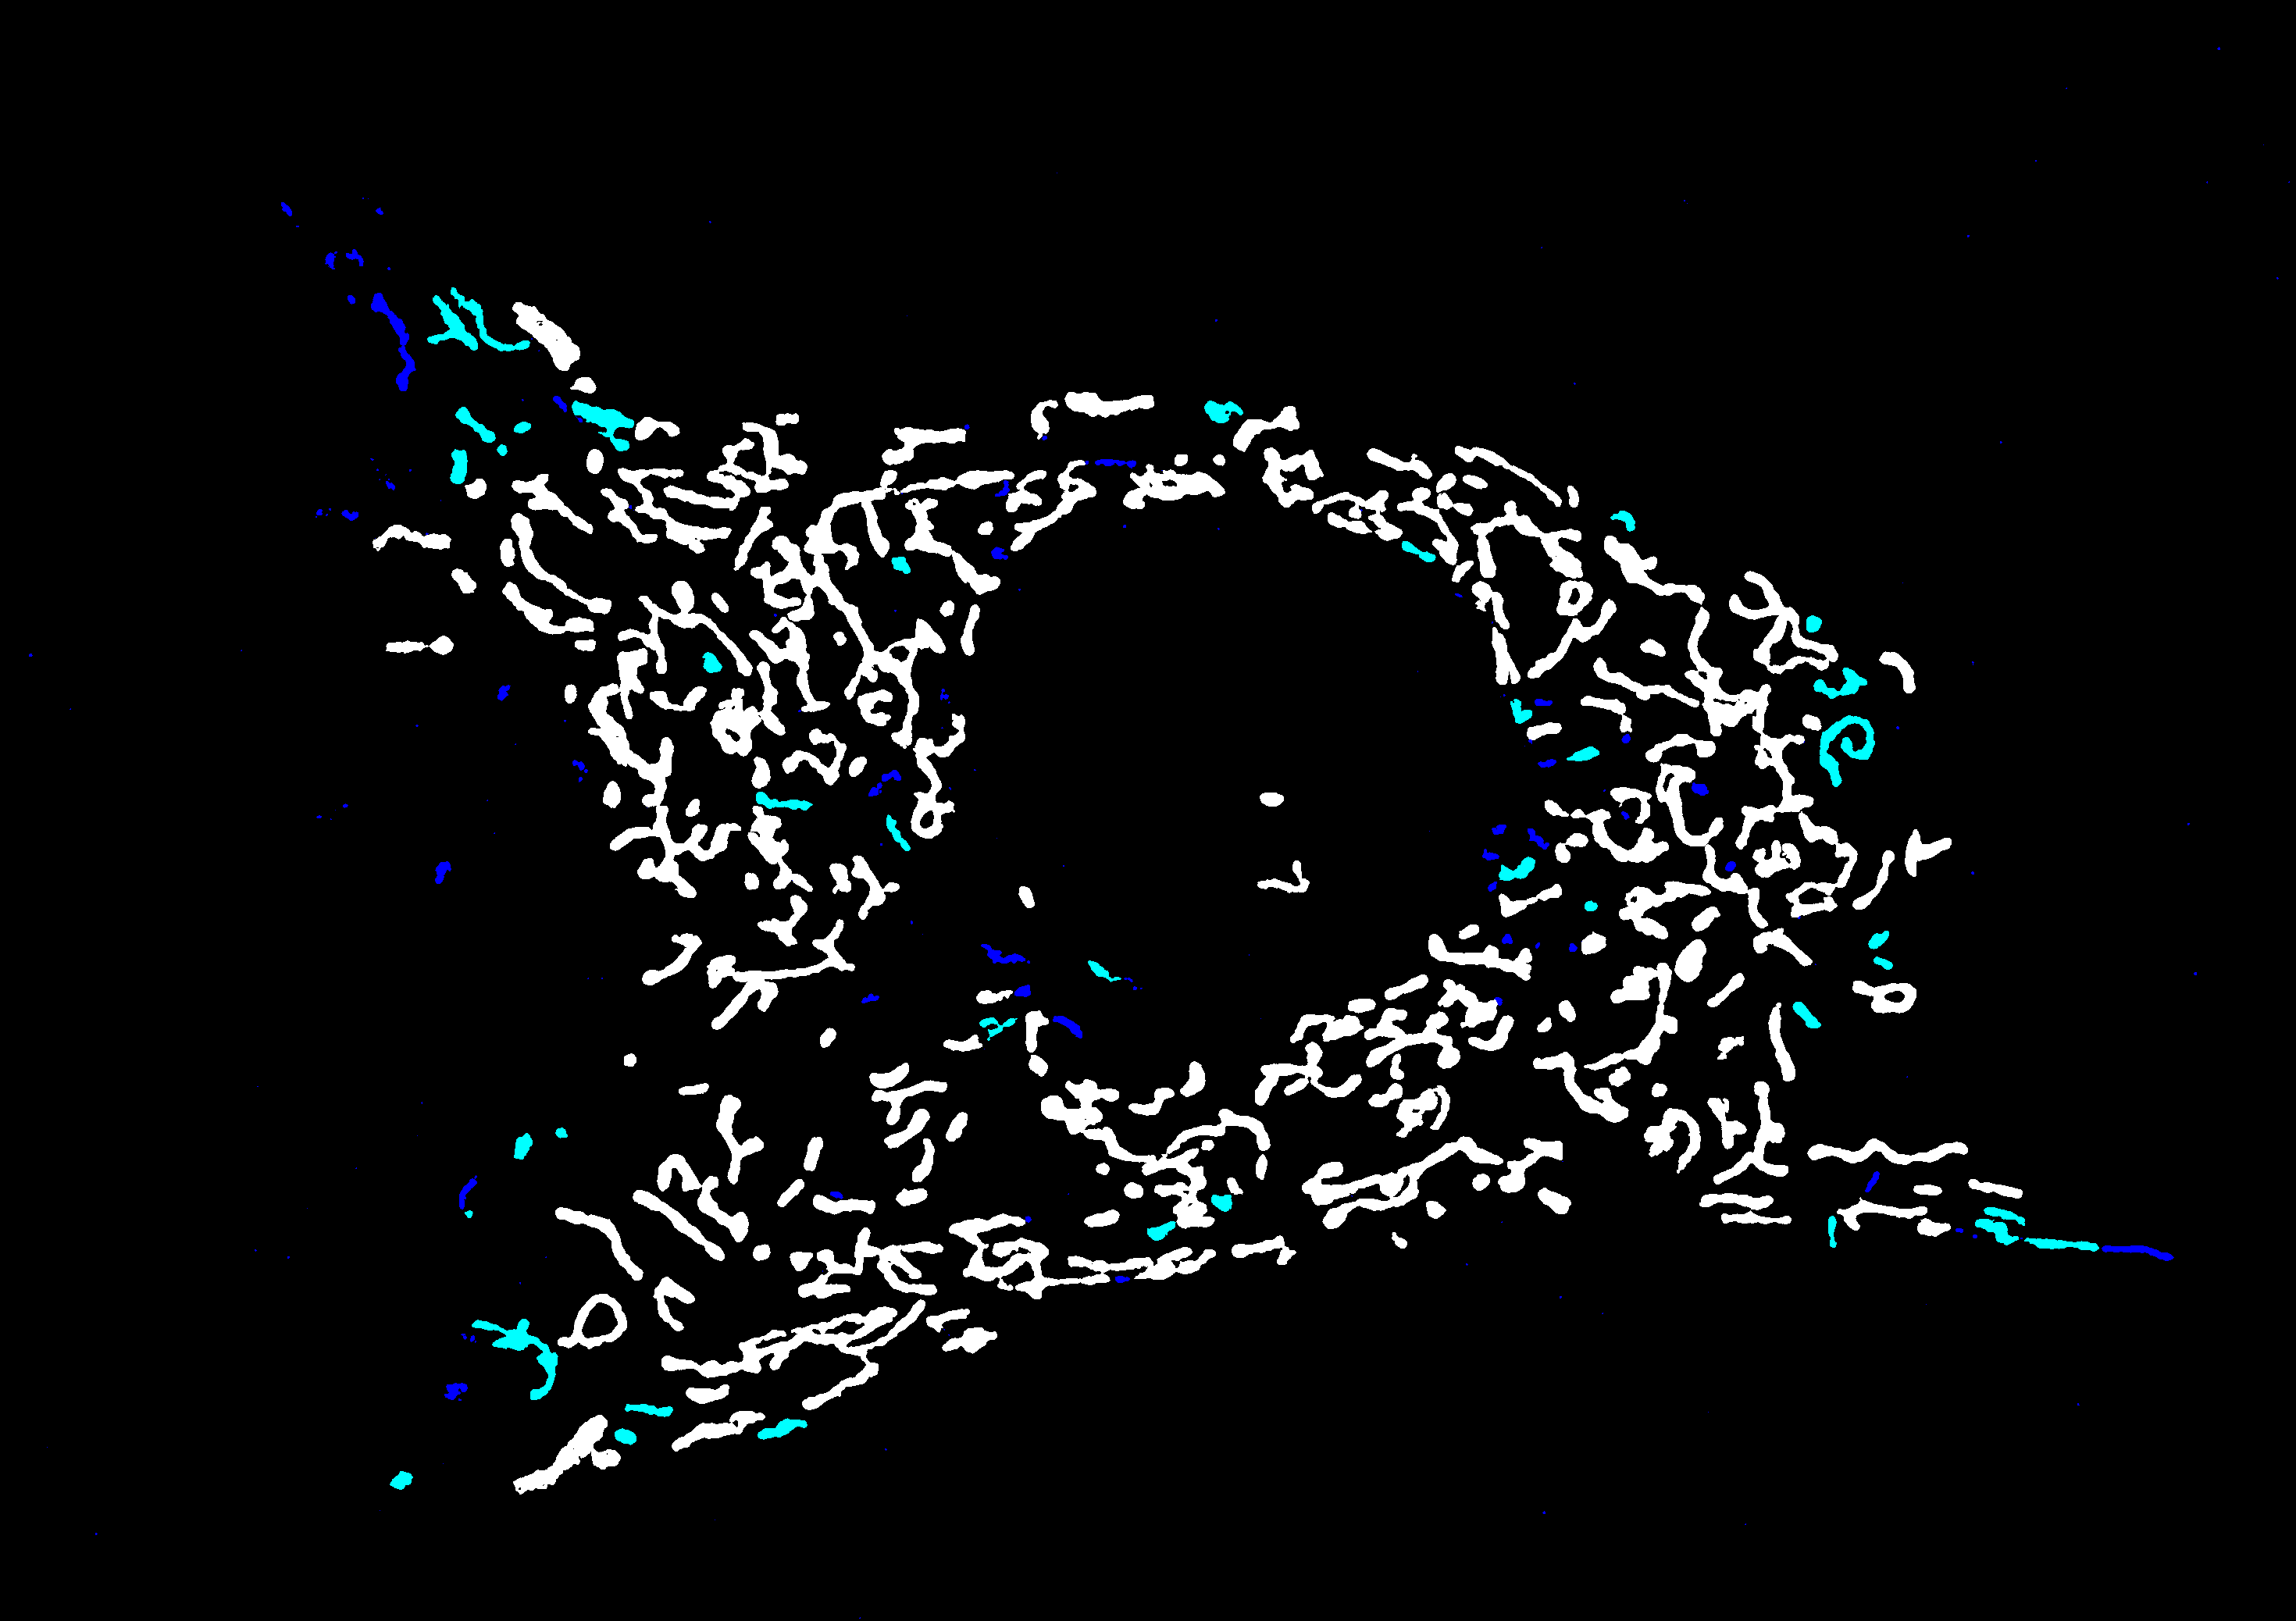
\includegraphics[width=0.39\textwidth]{figs/ch3figs/centroid_compare.png}}
    \label{fig:centroid_illustration}
    \caption[A comparison between the initial centroid method(incorrect centroid) and the robust method that is used (correct centroid)]{A comparison between the initial centroid method(incorrect centroid) and the robust method that is used (correct centroid). The difference in the centroid value outcome is illustrated on an inverted gradient distribution line plot where dashed vertical lines are used to illustrate the centroids while the difference in the impact on the Hysteresis thresholding results are displayed using a MIP image. The image is colour-coded to differentiate and aid in comparison between the threshold outcomes}
\end{figure}
%look up if there is any benefit due to the divider that is documented
%Mention that it is the more robust approach
%This is all we really have. Show two tot three diagrams for how this selects values and move one (we can't say why better so we test it [between the two centroid approaches])
\subsection{Applying biases to the centroid result}\label{sec:system_biases}
As it was found that at times the centroid result returned a high threshold that was too strict biases were developed to balance this. The reason for this is speculated to be due to the reduction in the context of the objects depicted in the image due to the quantification of image properties. Primarily is this IHH distribution which describes the response behaviour of the image to varied high threshold strictness but does not provide the nuance to know when it is relegating a large number of image structures to the background as opposed to the foreground nor can it consider properties such as the shape or volume of the individual potential foreground structures in an effective manner. To address this two biases were applied.

\subsubsection{IHH total volume bias}
So as to add some bias to the high threshold determined using the centroid a second weighting metric was added which was based on the normalized IHH distribution for the image. This is applied to the numerator and denominator within the summation as shown in Equation \ref{eq:vox_weight_added}. By doing so we introduce the context of the distribution of foreground information which the IHH describes as the $y$-axis representing the number of foreground voxels for each $x$-axis value representing the high threshold (therefore the strictness of the high threshold) resulting in an IHH weighting $v(n)$.
\begin{equation}\label{eq:vox_weight_added}
    C_x = \frac{\sum_{0}^{N-1} v(n)\circ \overline{y}'_{\text{new}}(n)\circ x(n)}{\sum_{0}^{N}\overline{y}'_{\text{new}}(n)\circ v(n)}
\end{equation}
The effect of this can be seen in Figure \ref{fig:distro_centroid_compare} where the difference between the centroid determined using the inverted gradient representation of the IHH can be greatly skewed by the application of the normalized IHH distribution. In this figure, the distributions (separated and combined) for two sample images deviate further from the separate centroids the faster the IHH distribution decays relative to the increasing high threshold intensity along the x-axis. This means that although the centroid of two IHH distributions can be close between two samples their influence on an identical inverted gradient distribution is less predictable. The benefit of this is that the strength of this bias is dependent on the distribution of the potential foreground structure information across the high threshold intensity span. Better separated foreground structures with a higher contrast will typically result in distinctly rectangular distributions or ones that decay in wider steps and are more robust to fluctuations in the high threshold value.\par
\begin{figure}
%This will be 4 graphs with two per sample. One graph type will have two overlayed lineplots (inverted and IHH with each having own centroid) and a second graph type for when the weighting is applied with the resulting new centroid. 
    \centering
    \subcaptionbox{Inverted and normalized IHH distributions for a sample A with dashed vertical lines for the centroids \label{subfig:separate_distrosA}}{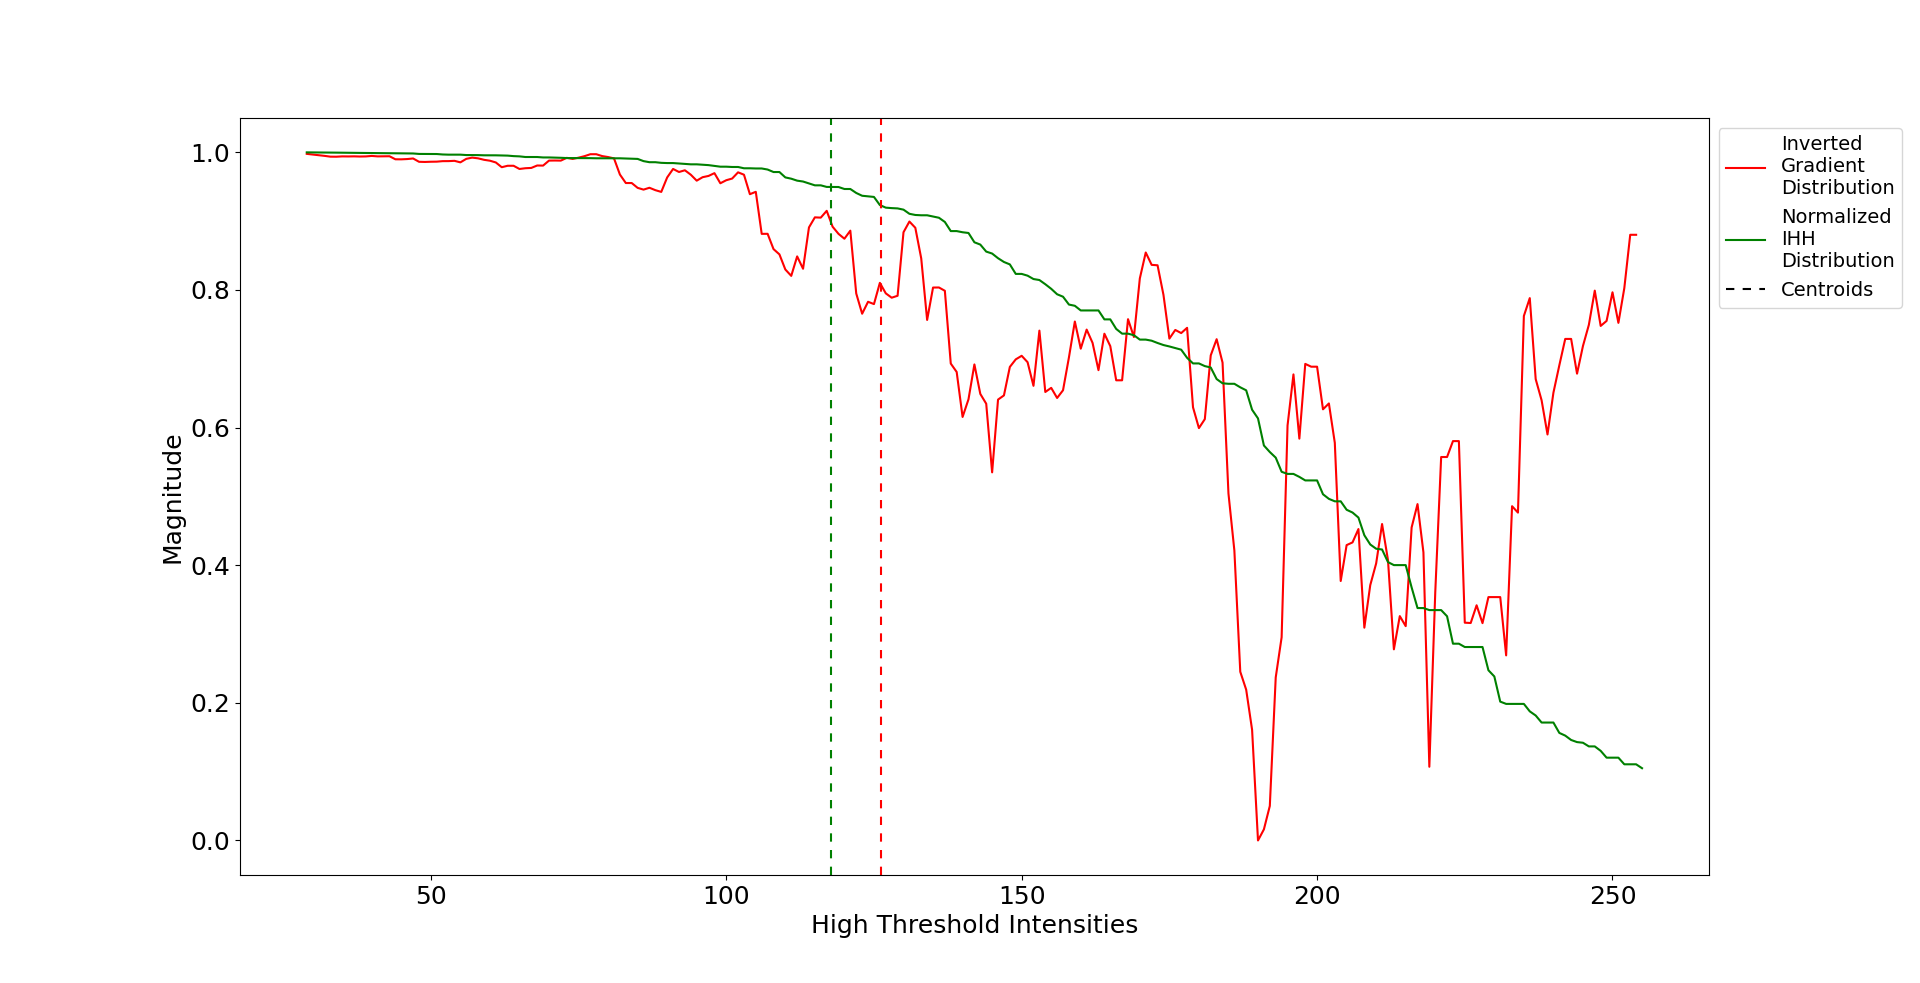
\includegraphics[width=0.49\textwidth]{figs/ch3figs/distros_with_centroids_separateA.png}}
    \subcaptionbox{The inverted gradient distribution with the normalized IHH weighting applied and a dashed vertical line representing the centroid for a sample A \label{subfig:combined_distroA}}{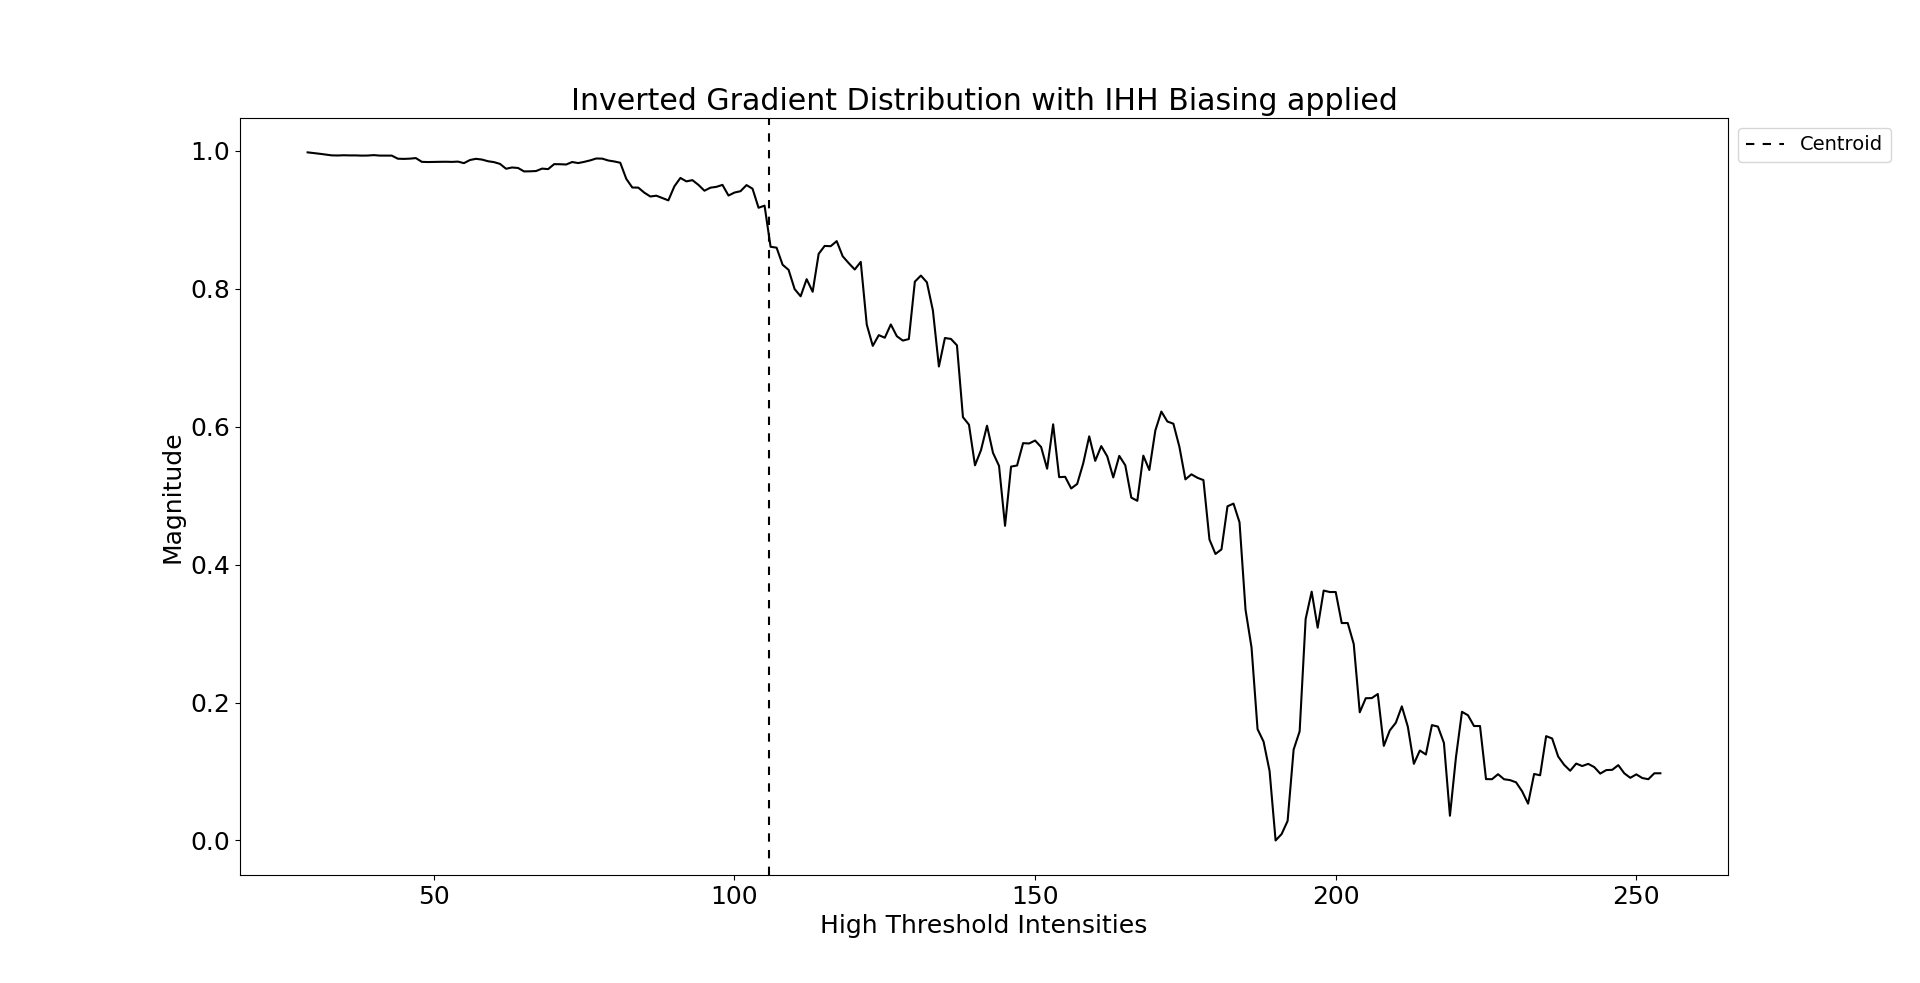
\includegraphics[width=0.49\textwidth]{figs/ch3figs/both_distro_combinedA.png}}
    \subcaptionbox{Inverted and normalized IHH distributions for a sample B with dashed vertical lines for the centroids \label{subfig:separate_distrosB}}{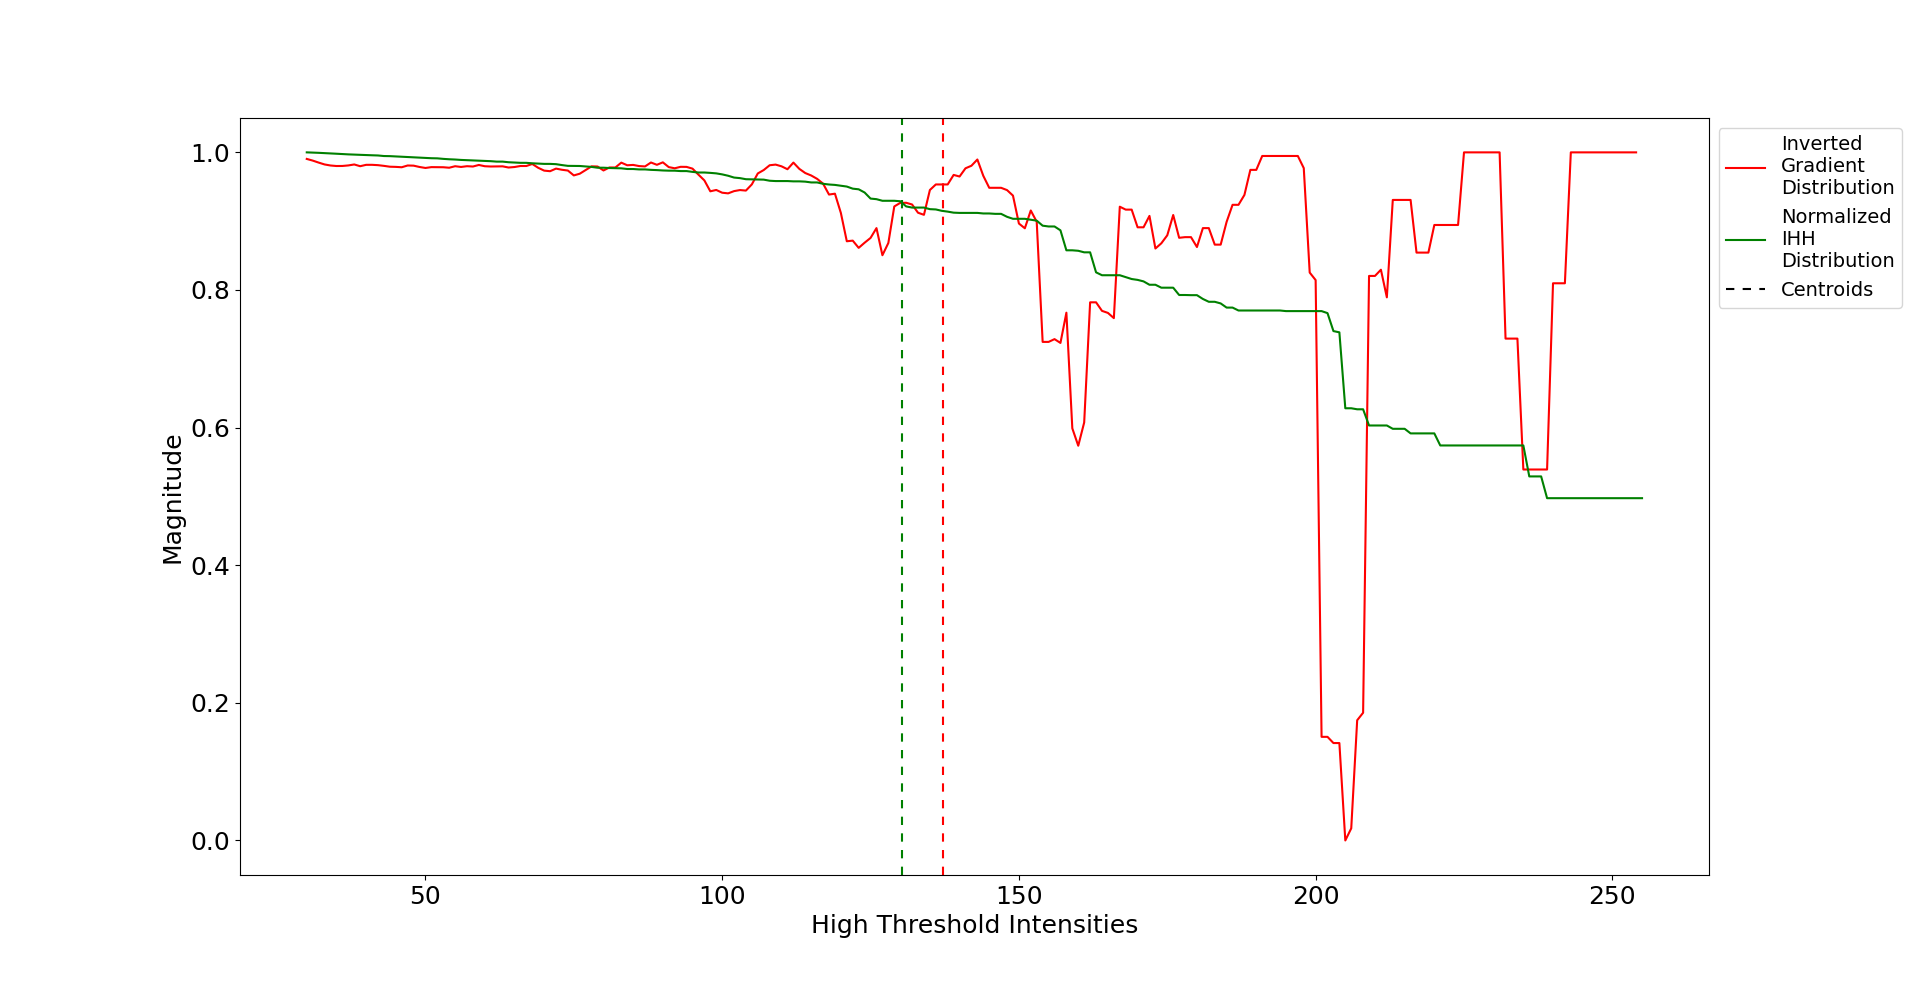
\includegraphics[width=0.49\textwidth]{figs/ch3figs/distros_with_centroids_separateB.png}}
    \subcaptionbox{The inverted gradient distribution with the normalized IHH weighting applied and a dashed vertical line representing the centroid for a sample B \label{subfig:combined_distroB}}{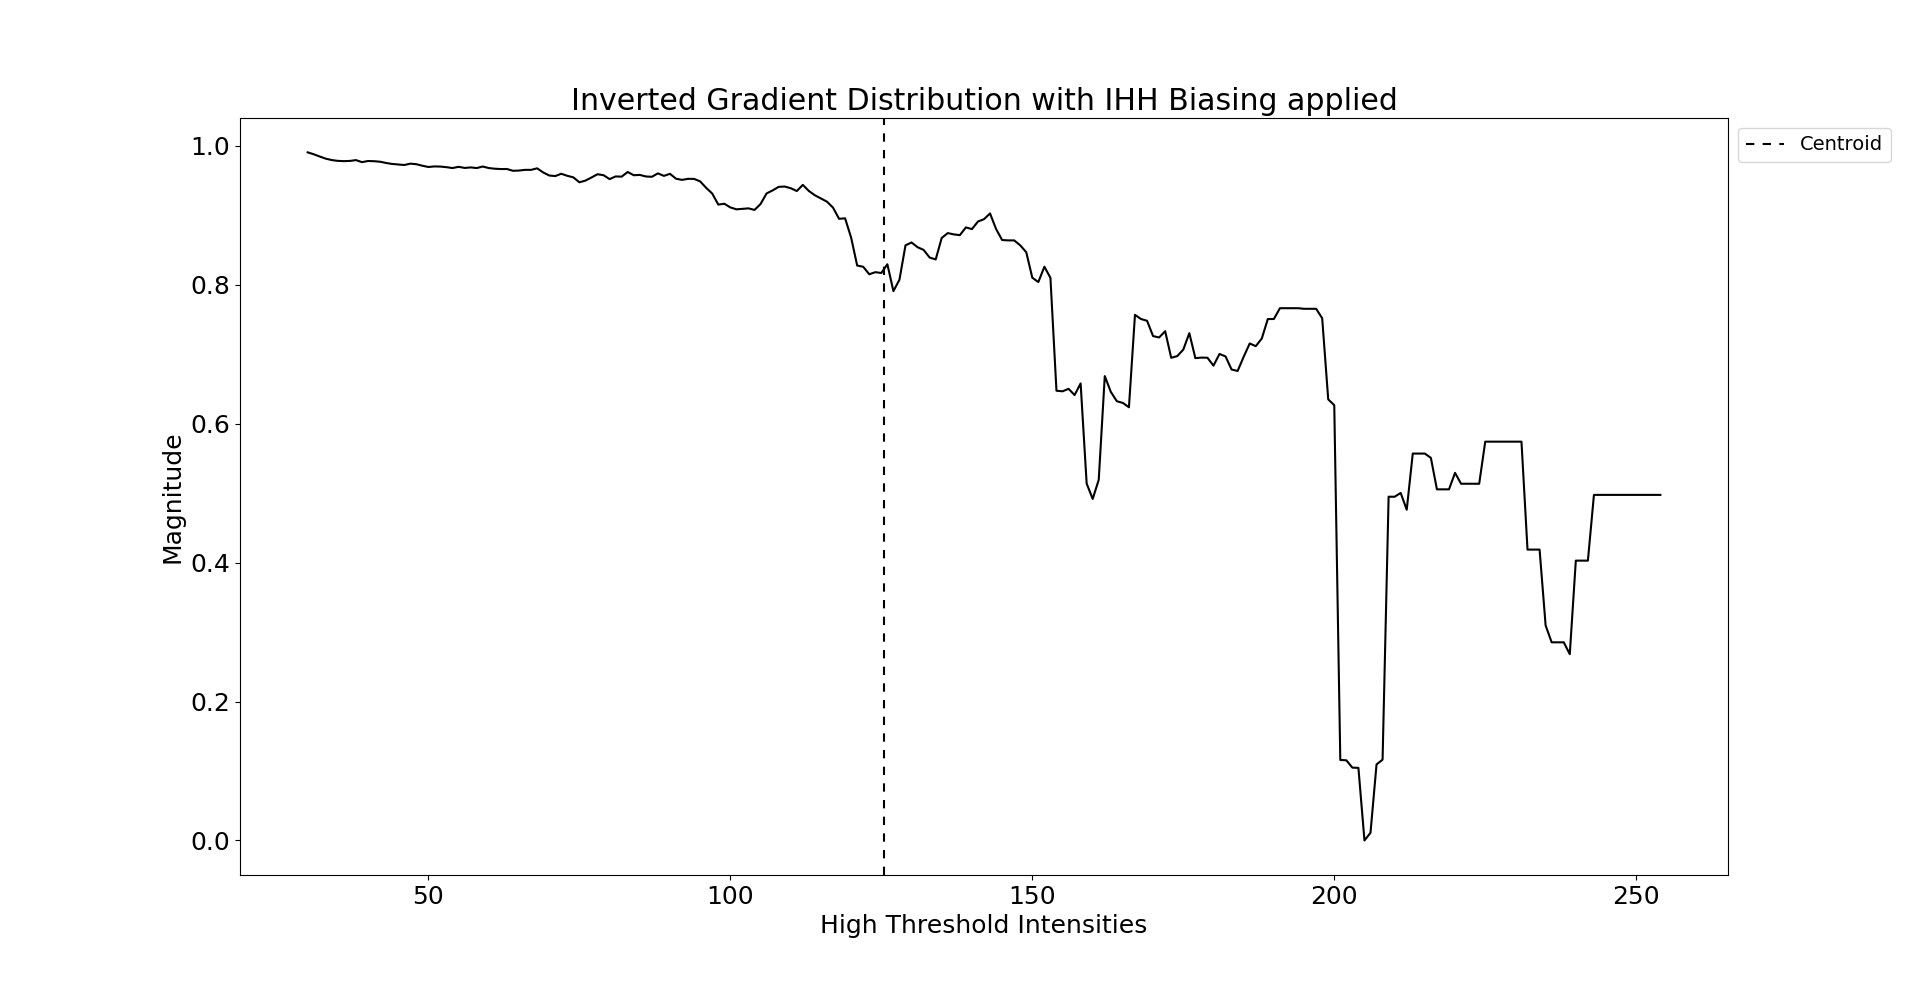
\includegraphics[width=0.49\textwidth]{figs/ch3figs/both_distro_combinedB.png}}
    \caption[A showcase comparing the influences of the inverted gradient and normalized IHH distributions on the centroids separately and when combined]{A showcase comparing the influences of the inverted gradient and normalized IHH distributions on the centroids separately and when combined. In the figures illustrating both the separate distributions in red and green (Fig. \ref{subfig:separate_distrosA} \& \ref{subfig:separate_distrosB}) and the new distribution produced by multiplying said distributions and determining a new centroid (Fig. \ref{subfig:combined_distroA} \& \ref{subfig:combined_distroB}). By comparing the change in the determined centroids when the distributions are combined for Samples A (Fig. \ref{subfig:separate_distrosA} \& \ref{subfig:combined_distroA}) and B (Fig. \ref{subfig:separate_distrosB} \& \ref{subfig:combined_distroB}) it can be observed that the new centroid determined in the former sample is at a lower value than either of the separate centroids while for the latter sample the new centroid is far closer to the separate centroids of the original distributions. This highlights the impact the shape of the distribution has on the calculated centroid value.}
    \label{fig:distro_centroid_compare}
\end{figure}
The reason for this is the leniency towards false positives over false negatives for foreground selection as erroneously labelled foreground can be removed with further processing yet the background erroneously labelled background is typically lost to further analysis. Since the high threshold selection is expected to be a best-fit approximation, tending towards a precise value, it is supposed that there will be some level of error and despite a goal being to minimize this error it was decided that it would rather err to a lower high threshold value as opposed to a higher value. A fixed shift in the approximated towards the lower intensity values was deemed inapplicable as it is naive to the imaging conditions and uniqueness presented by each sample image and no single value would work, this shift would need to adapt to the image. This is the reason that the IHH was chosen since tending the high threshold range towards the lower end typically results in a plateau or increase in IHH magnitude implying an increase in potential foreground information. As we tend to a lower high threshold value the risk of the potential foreground voxels being that of noise increases relatively speaking thus this is used in conjunction with the inverted gradient representation of the IHH with the intention that each compensates for the other.
\begin{figure}
%This will contain the raw MIP of one sample from above. There will be a structure highlighting MIP as well. An RGB overlay of the normal centroid (R) and the centroid from just the IHH (G). Lastly, there will be a viridis MIP showing the new centroid effect combined with structure highlighting. This way the graphs don't have to be shown again and only MIP displayed
    \centering
    \subcaptionbox{Raw image with no thresholds applied\label{subfig:mip_centroid_compareA}}{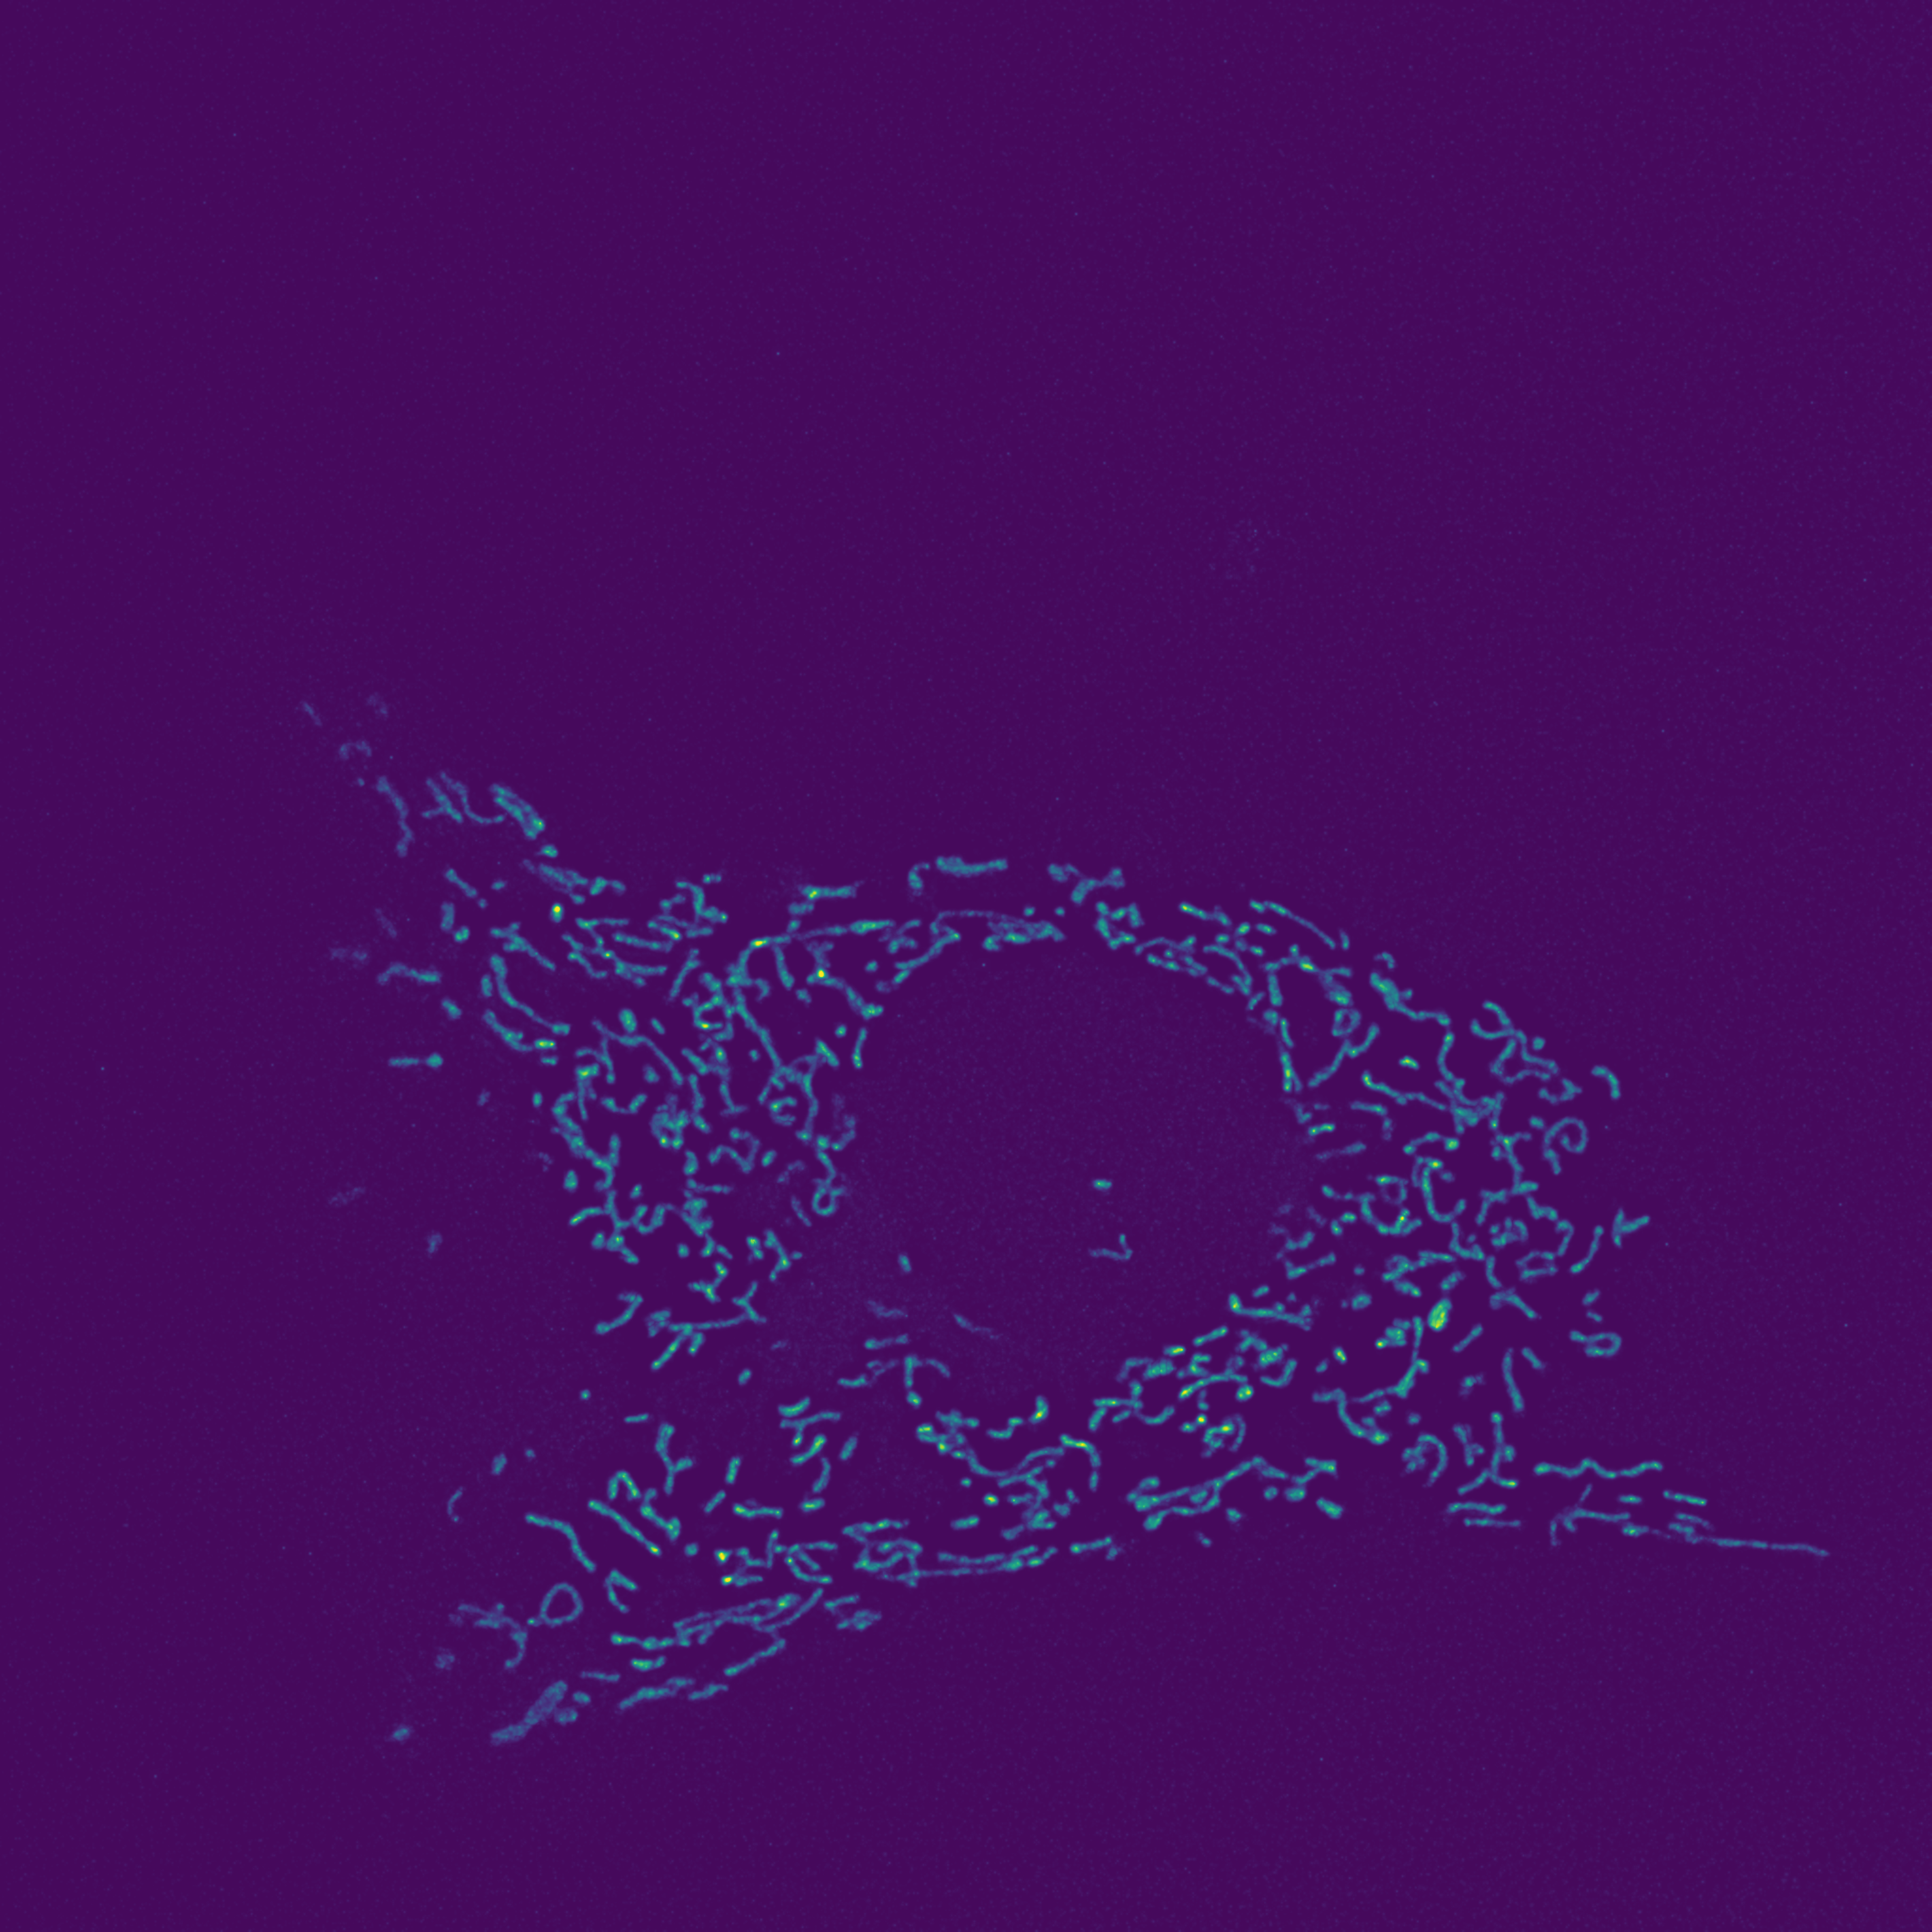
\includegraphics[width=0.49\textwidth]{figs/ch3figs/raw_mip.png}}
    \subcaptionbox{The potential foreground structures are highlighted with different colours based on the maximum voxel intensity contained within after a low threshold has been applied\label{subfig:mip_centroid_compareB}}{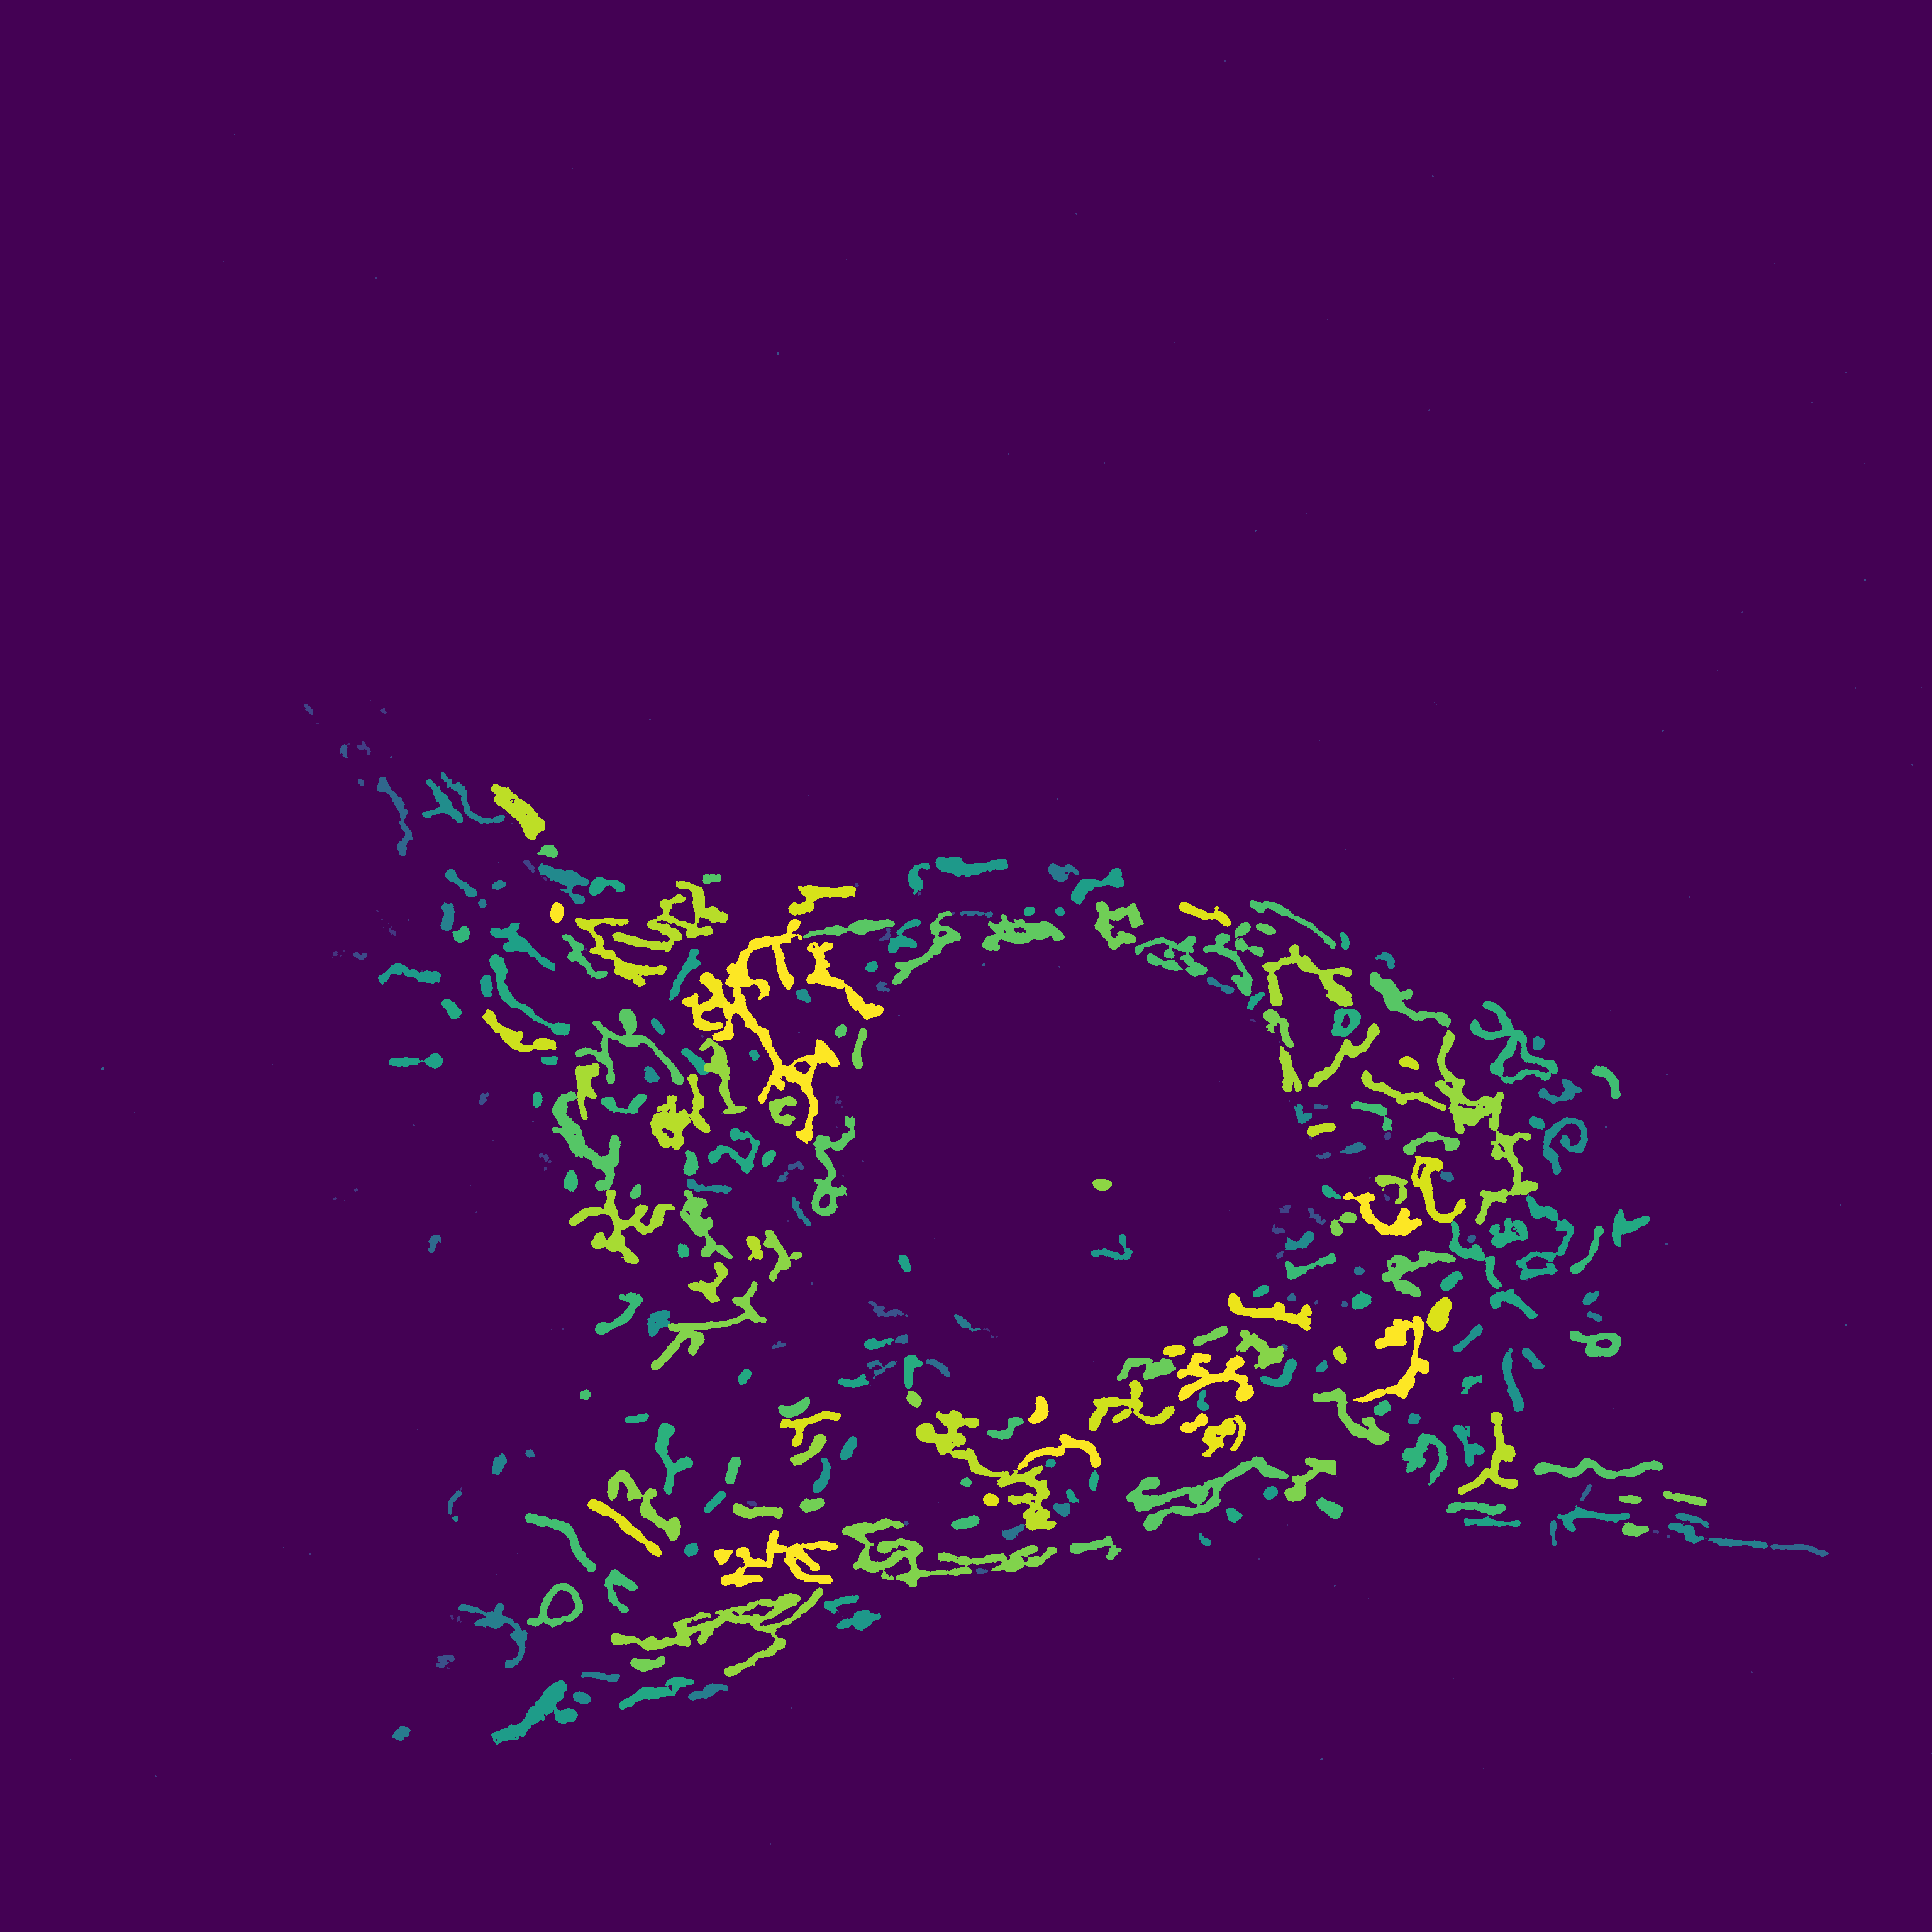
\includegraphics[width=0.49\textwidth]{figs/ch3figs/highlight_mip.png}}
    \subcaptionbox{A red, green and blue (RGB) each colour channel labels regions above a specific threshold. The red, green, and blue channels represent the voxels of structures containing an intensity greater than that of the threshold derived using the inverted gradient distribution, the IHH distribution, and the product of both distributions respectively. The cyan regions are where green and blue overlap and the grayscale regions are where all three channels overlap.\label{subfig:mip_centroid_compareC}}{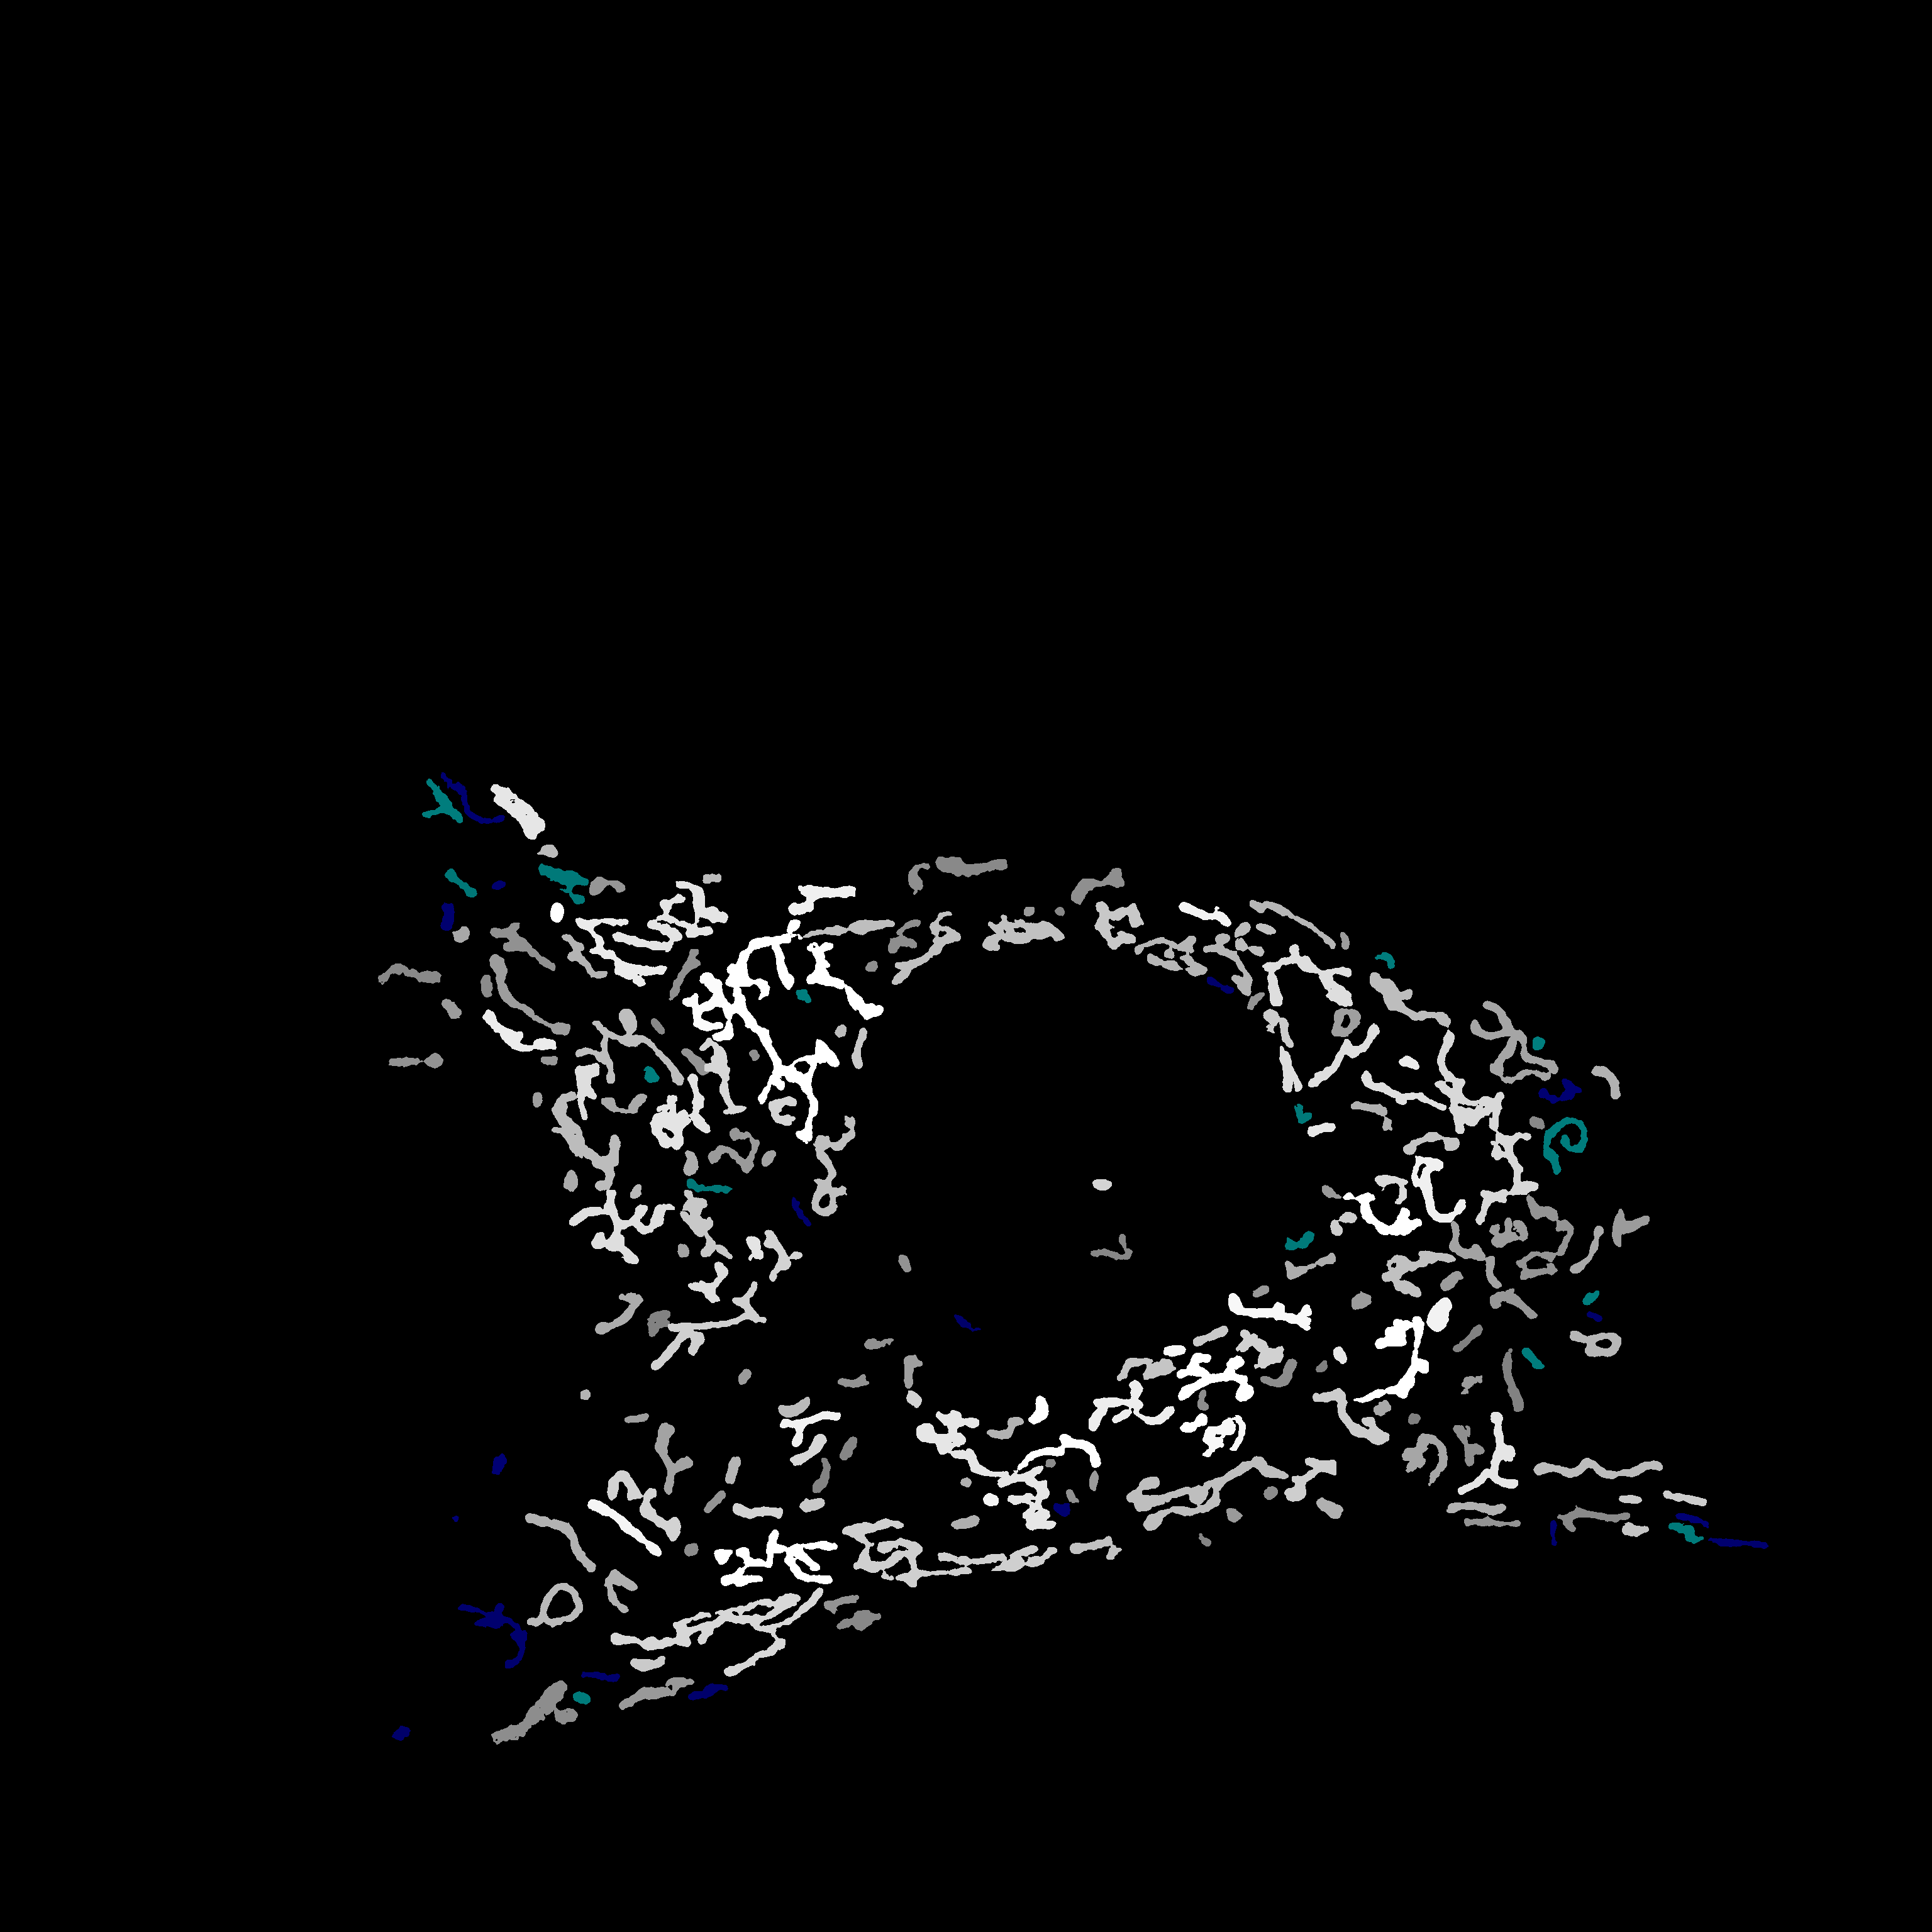
\includegraphics[width=0.49\textwidth]{figs/ch3figs/rg_mip.png}}
    \subcaptionbox{The structures are colour-coded according to the maximum structure intensity of each. The structures remaining are those that have a maximum intensity greater than the centroid of the inverted gradient distribution after the normalized IHH distribution has been applied as weighting\label{subfig:mip_centroid_compareD}}{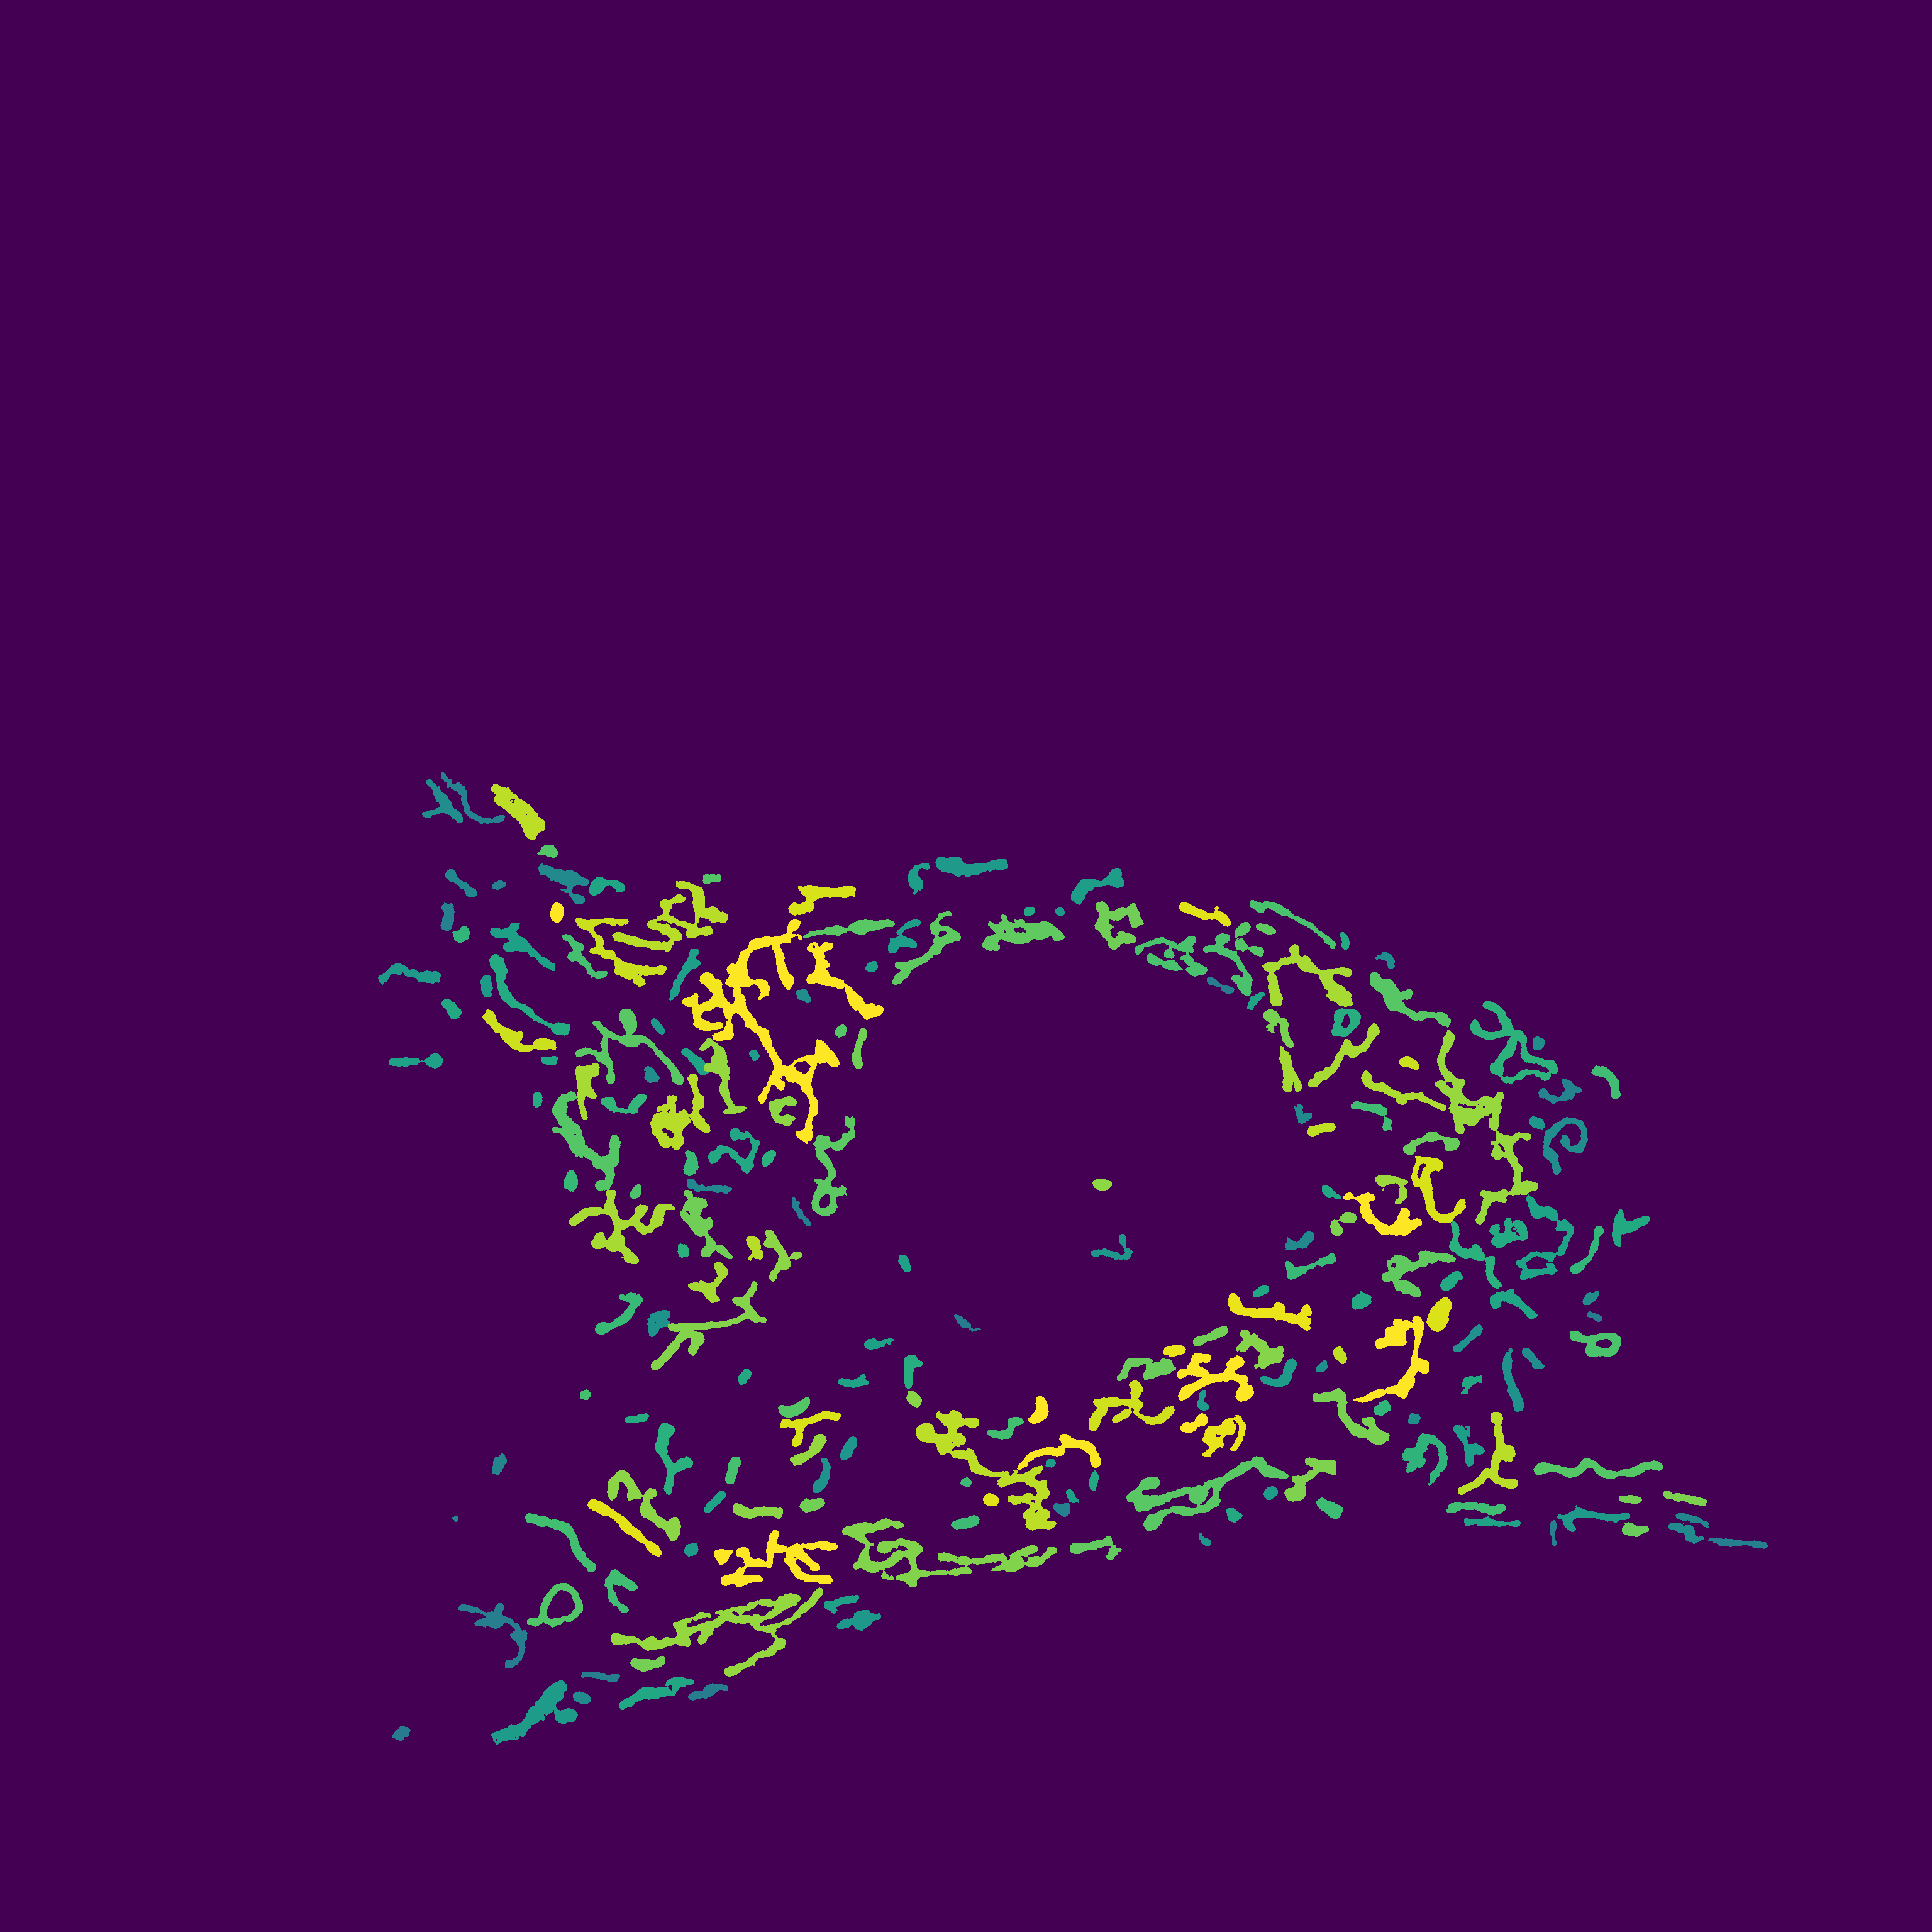
\includegraphics[width=0.49\textwidth]{figs/ch3figs/weighted_mip.png}}
    \caption{The images shown are MIP images of a sample image where the differences of the different centroids, determined using the relevant distributions, are illustrated.\label{fig:centroid_weighting_mips} \textcolor{red}{I feel the caption of the RGB subfigure is a bit too long, do you have any suggestions? Perhaps I should summarize the subfigure captions and move the descriptions to the main caption?}}
\end{figure}
Figure \ref{fig:centroid_weighting_mips} illustrates the effect of these different centroid results on the hysteresis thresholding outcome. The distributions shown in Figure \ref{fig:distro_centroid_compare} (\subref{subfig:separate_distrosA}) and (\subref{subfig:combined_distroA}) are for this same sample image and in the red and green centroids shown in (\subref{subfig:separate_distrosA}) match to the red and green colour channels shown in Figure \ref{subfig:mip_centroid_compareC} (red and green overlap appears as yellow). Despite the green channel threshold (based on the IHH distribution centroid) being lower than that of the red channel the final centroid calculated from the IHH weighted inverted gradient distribution (Fig. \ref{subfig:combined_distroA}) contains more structures than even the green channel as the centroid value is of an even lower value. This will provide a bias which will provide a lower high threshold intensity than the inverted gradient distribution along with the magnitude of this bias being image dependent meaning that the bias adapts to the sample image as opposed to some fixed value that needs to be entered for each sample.

\subsubsection{Shrinking window bias}
A second kind of bias that was implemented was the sliding window bias which affects the distribution for which the spectral centroid is calculated. This base premise is that within the intensity range above the low threshold, the lowest intensity value is supposed to be to the left while the highest intensity is to the right where the window initially spans from the furthest left with the upper range of the window ($I$) iterating across the range $I=[x_{min}+1, X]$. This range begins at $x_{min}+1$ which is 1 value greater than the smallest value within the original range after the low threshold application thus the lowest intensity value is not necessarily $0$. This is described in Equation \ref{eq:window_centroid}, and illustrated in Figure \ref{fig:window_approach}, which shows how the centroid ($C_I$) would be calculated for a window with an intensity upper bound of $I$ where in this figure there are three windows shown, with the respective centroids, with varied window sizes to illustrate the effect on the centroid value a narrower distribution has. This can be applied in conjunction with the IHH total volume bias with $\overline{y}'_{\text{new}}$ substituted for $v_w(i)\circ \overline{y}'_{\text{new}}(i)$.
\begin{equation}\label{eq:window_centroid}
    C_I(d) = \frac{\sum_{i=x_{min}}^{d} \overline{y}'_{\text{new}}(i)\circ x(i)}{\sum_{i=x_{min}}^{d}\overline{y}'_{\text{new}}(i)} \text{ where } d \leq X \text{ and } d \subset X
\end{equation}
\begin{figure}
%This will be a figure where an annotation will be made for the hypothetical window frame using I for the window and (X-I) for the excluded part outside the window. The original centroid could be shown and the window centroid will be shown as well using dashed lines
    \centering
    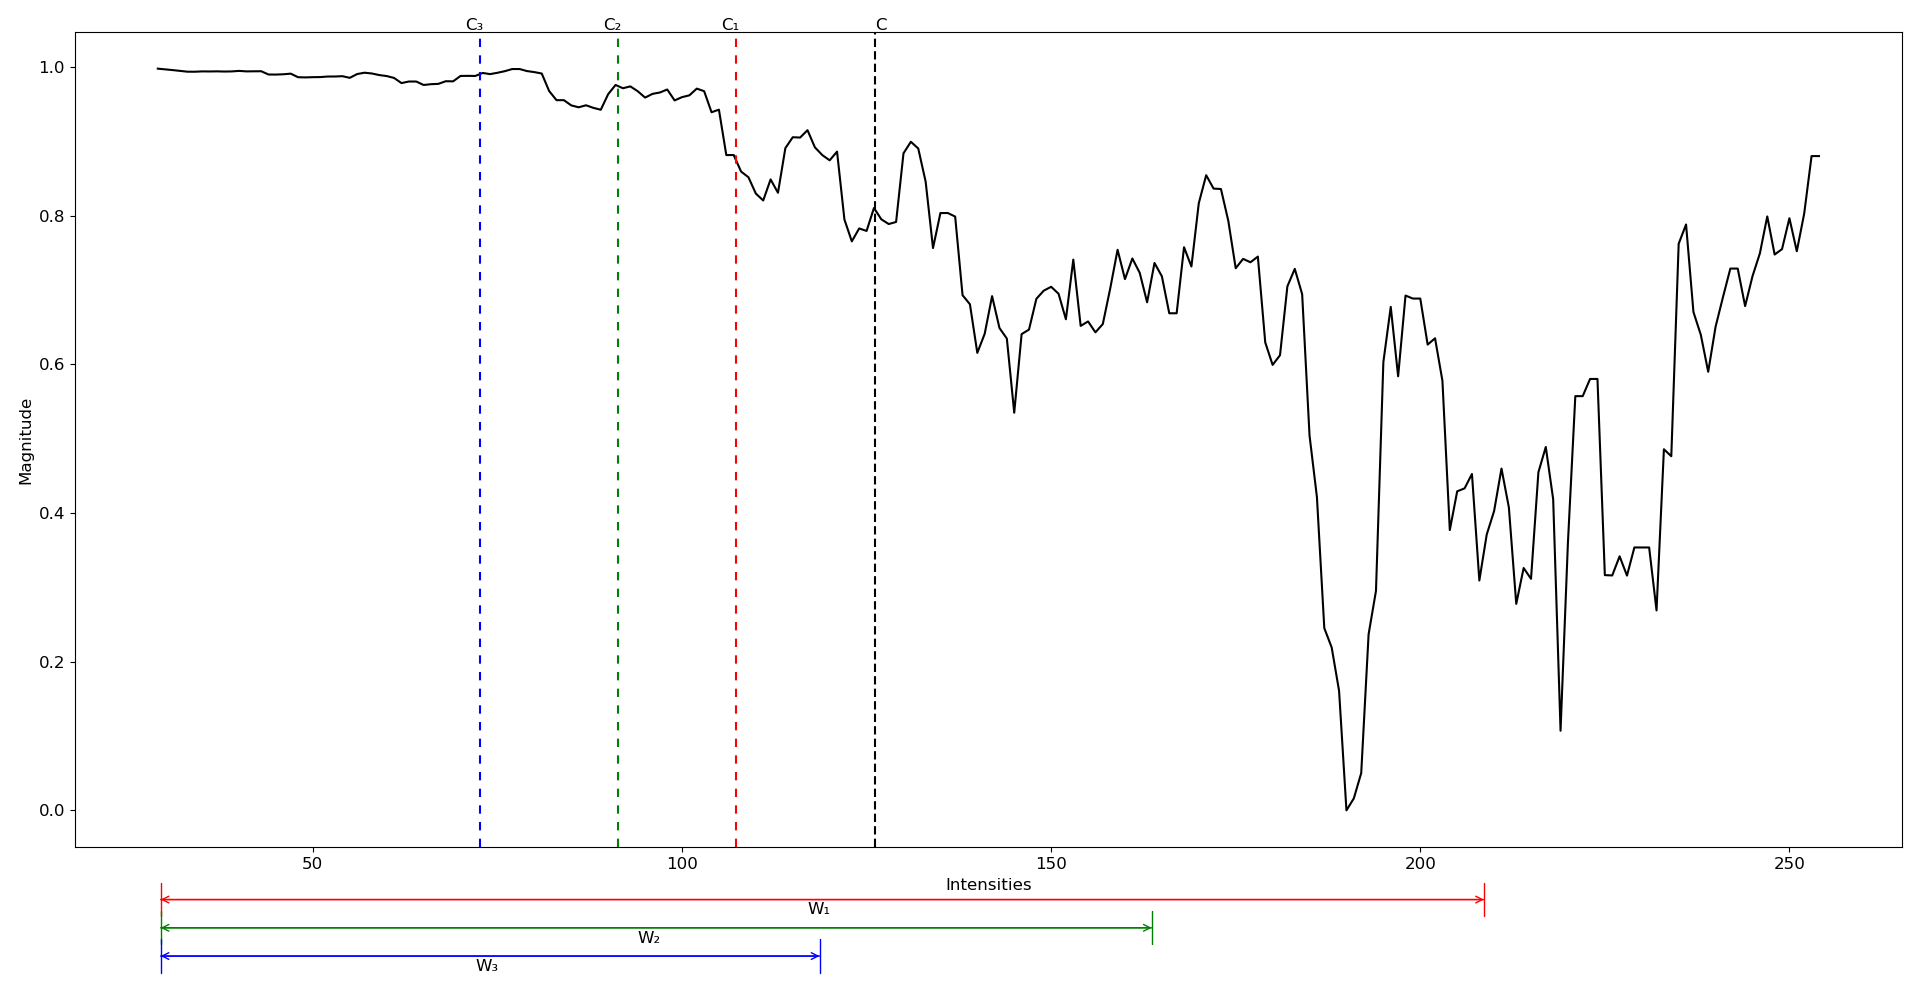
\includegraphics[width=\textwidth]{figs/ch3figs/Windows_overlapping.png}
    \caption[An example of how the window weighting approaches are applied to the distributions]{An example of how the window weighting approaches are applied to the distributions where in this example there are three bounded windows shown. The spans of these windows are annotated below the x-axis using coloured, horizontal lines with an accompanied label where window 1 ($W_1$) is shown with red, window 2 ($W_2$) is shown with green, and window 3 ($W_3$) is shown with blue. Each of these windows also has a respective centroid calculated for the distribution that falls within the window range which is annotated by a dashed vertical line with the appropriate colouring to match the windows and a label $C_n$ where $n$ is for the respective window. There is a black dashed vertical line with the label $C$ which represents the distribution centroid for the whole distribution without the windows}
    \label{fig:window_approach}
\end{figure}
As mentioned, this function will be performed for each iteration of $I$ resulting in numerous windowed centroids $C_I(I)$ across the window width range which will tend toward the lower intensity as the window width shrinks and contain less higher intensity components but the degree to which they veer to the lower intensities is also subject to the distribution contained within the window. What is crucial is the manner by which these windowed centroids are consolidated to a singular value to act as the high threshold. Taking the straight average was initially considered but due to the windows reducing the total context provided by the image distributions (IHH or inverted gradient), it was believed that the contributions of each window could not be received equally towards the final value. It is for this reason that two consolidation approaches were developed with the goal of effectively weighting the contribution of each window centroid to the final high threshold value settled on. The consolidated window weighted centroid ($C_W$) is shown in Equation \ref{eq:window_weighting} where the weighted average of the window centroids ($C_I$) using the window weights ($w$) but these weights are dependent on the weighting functions described in the consolidation approaches.
\begin{equation}\label{eq:window_weighting}
    C_W = \frac{\sum_{t=x_{min}}^X C_I(t)\times w(t)}{\sum_{t=x_{min}}^X w(t)}
\end{equation}
The window weighting consolidation approaches are the \textbf{window width weighting} approach and the \textbf{window mass weighing} approach.
\paragraph{Window width weighting} is an approach where the weighting coefficient ($w$) that is applied for the consolidation is based on the current size of the window relative to the total width of the distribution. This is shown in Equation \ref{eq:win_width_weight} where $t$ is the current upper bound of the window and serves as the dependent variable, $w(t)$ is the window weighting to be used for consolidation, $X$ is the maximum intensity of distribution range, and $x_{min}$ is the minimum intensity of the distribution range as all intensities less than this have been remove by the low threshold.   
\begin{equation}\label{eq:win_width_weight}
    w(t) = \frac{t-x_{min}}{X-x_{min}}\text{ where } X \geq t > x_{min}
\end{equation}
This weighting approach provides a linearly decreasing weight function proportional to the loss of information provided by the distribution as the window shrinks. This results in a predictable weighting outcome for each window but it is believed that it is still somewhat naive to the information loss. 

\paragraph{Window mass weighting} is the approach where the weighting of each window centroid is weighed by the contained mass within the window relative to the total mass across the distribution. In this context, the "mass" can be derived by the total area under the distribution curve and the window mass is the area within the window bounds. Both of these areas are calculated by the sum of magnitudes ($\overline{y}'_{\text{new}}$) within the respective bounds ($t$ and $X$) and the division of the windowed area by the total area results in a window mass ratio as shown in Equation \ref{eq:window_mass_weight} which is used as the window consolidation weighting ($w(t)$).  
\begin{equation}\label{eq:window_mass_weight}
    w(t) = \frac{\sum_{i=x_{min}}^t \overline{y}'_{\text{new}}(i)}{\sum_{i=x_{min}}^X \overline{y}'_{\text{new}}(i)}
\end{equation}
With the added consideration of the "mass" contained within the window relative to the whole distribution, it is believed that this should provide a better weight for consolidation. The reason for this is that it is known that the greater the magnitude of the distribution at specific regions the more it shifts the centroid towards it and the greater the cluster of magnitude (large magnitude over a large area) the greater the contributor. Suppose that there is a high-intensity region of low magnitude such that it contributes only 10\% collectively to the centroid outcome, given this the loss of said region by windowing will be of little impact as even when included it was a negligible contributor. It is under this reasoning that the weighting is derived where the weighting of a window is relative to the measure of influence said region of the distribution has over the centroid relative to the entire centroid. The caveat is that the window weighting has a non-linearly decreasing weighting function $w(t)$ but is believed to be less naive than the window width weighting.\paragraph{Overall} the impact of the window weighting approaches on the high threshold acquisition is displayed in Figure \ref{fig:window_mips} where the contrast between no window methods being applied to either method being applied can be seen as the quantity of non-zero structures in Fig. \ref{subfig:window_weight_b} (high threshold is 155) is far less than either Fig. \ref{subfig:window_weight_c} or Fig. \ref{subfig:window_weight_d} (high threshold is 112 and 117 respectively). What is notable for this example is that the difference in high threshold results for the \textbf{window width} and \textbf{window mass} weightings are not that different but this is not necessarily the normality as the window weighting approaches are arguably more sensitive to the change in the shape of the distribution across the intensity range as it is a consolidation of numerous centroids thus compounding this "sensitivity" to the shape.

\begin{figure}
%This figure will have 4 images. These will be the image above the low threshold, the image above the low threshold with structure highlighting and a colorbar, the binarized outcome using weighting approach A, and the binarized outcome using weighting approach B. In the caption of the figure the high threshold determined by each approach must be listed so it can be compared
    \centering
    \subcaptionbox{The image with only the low threshold applied\label{subfig:window_weight_a}}{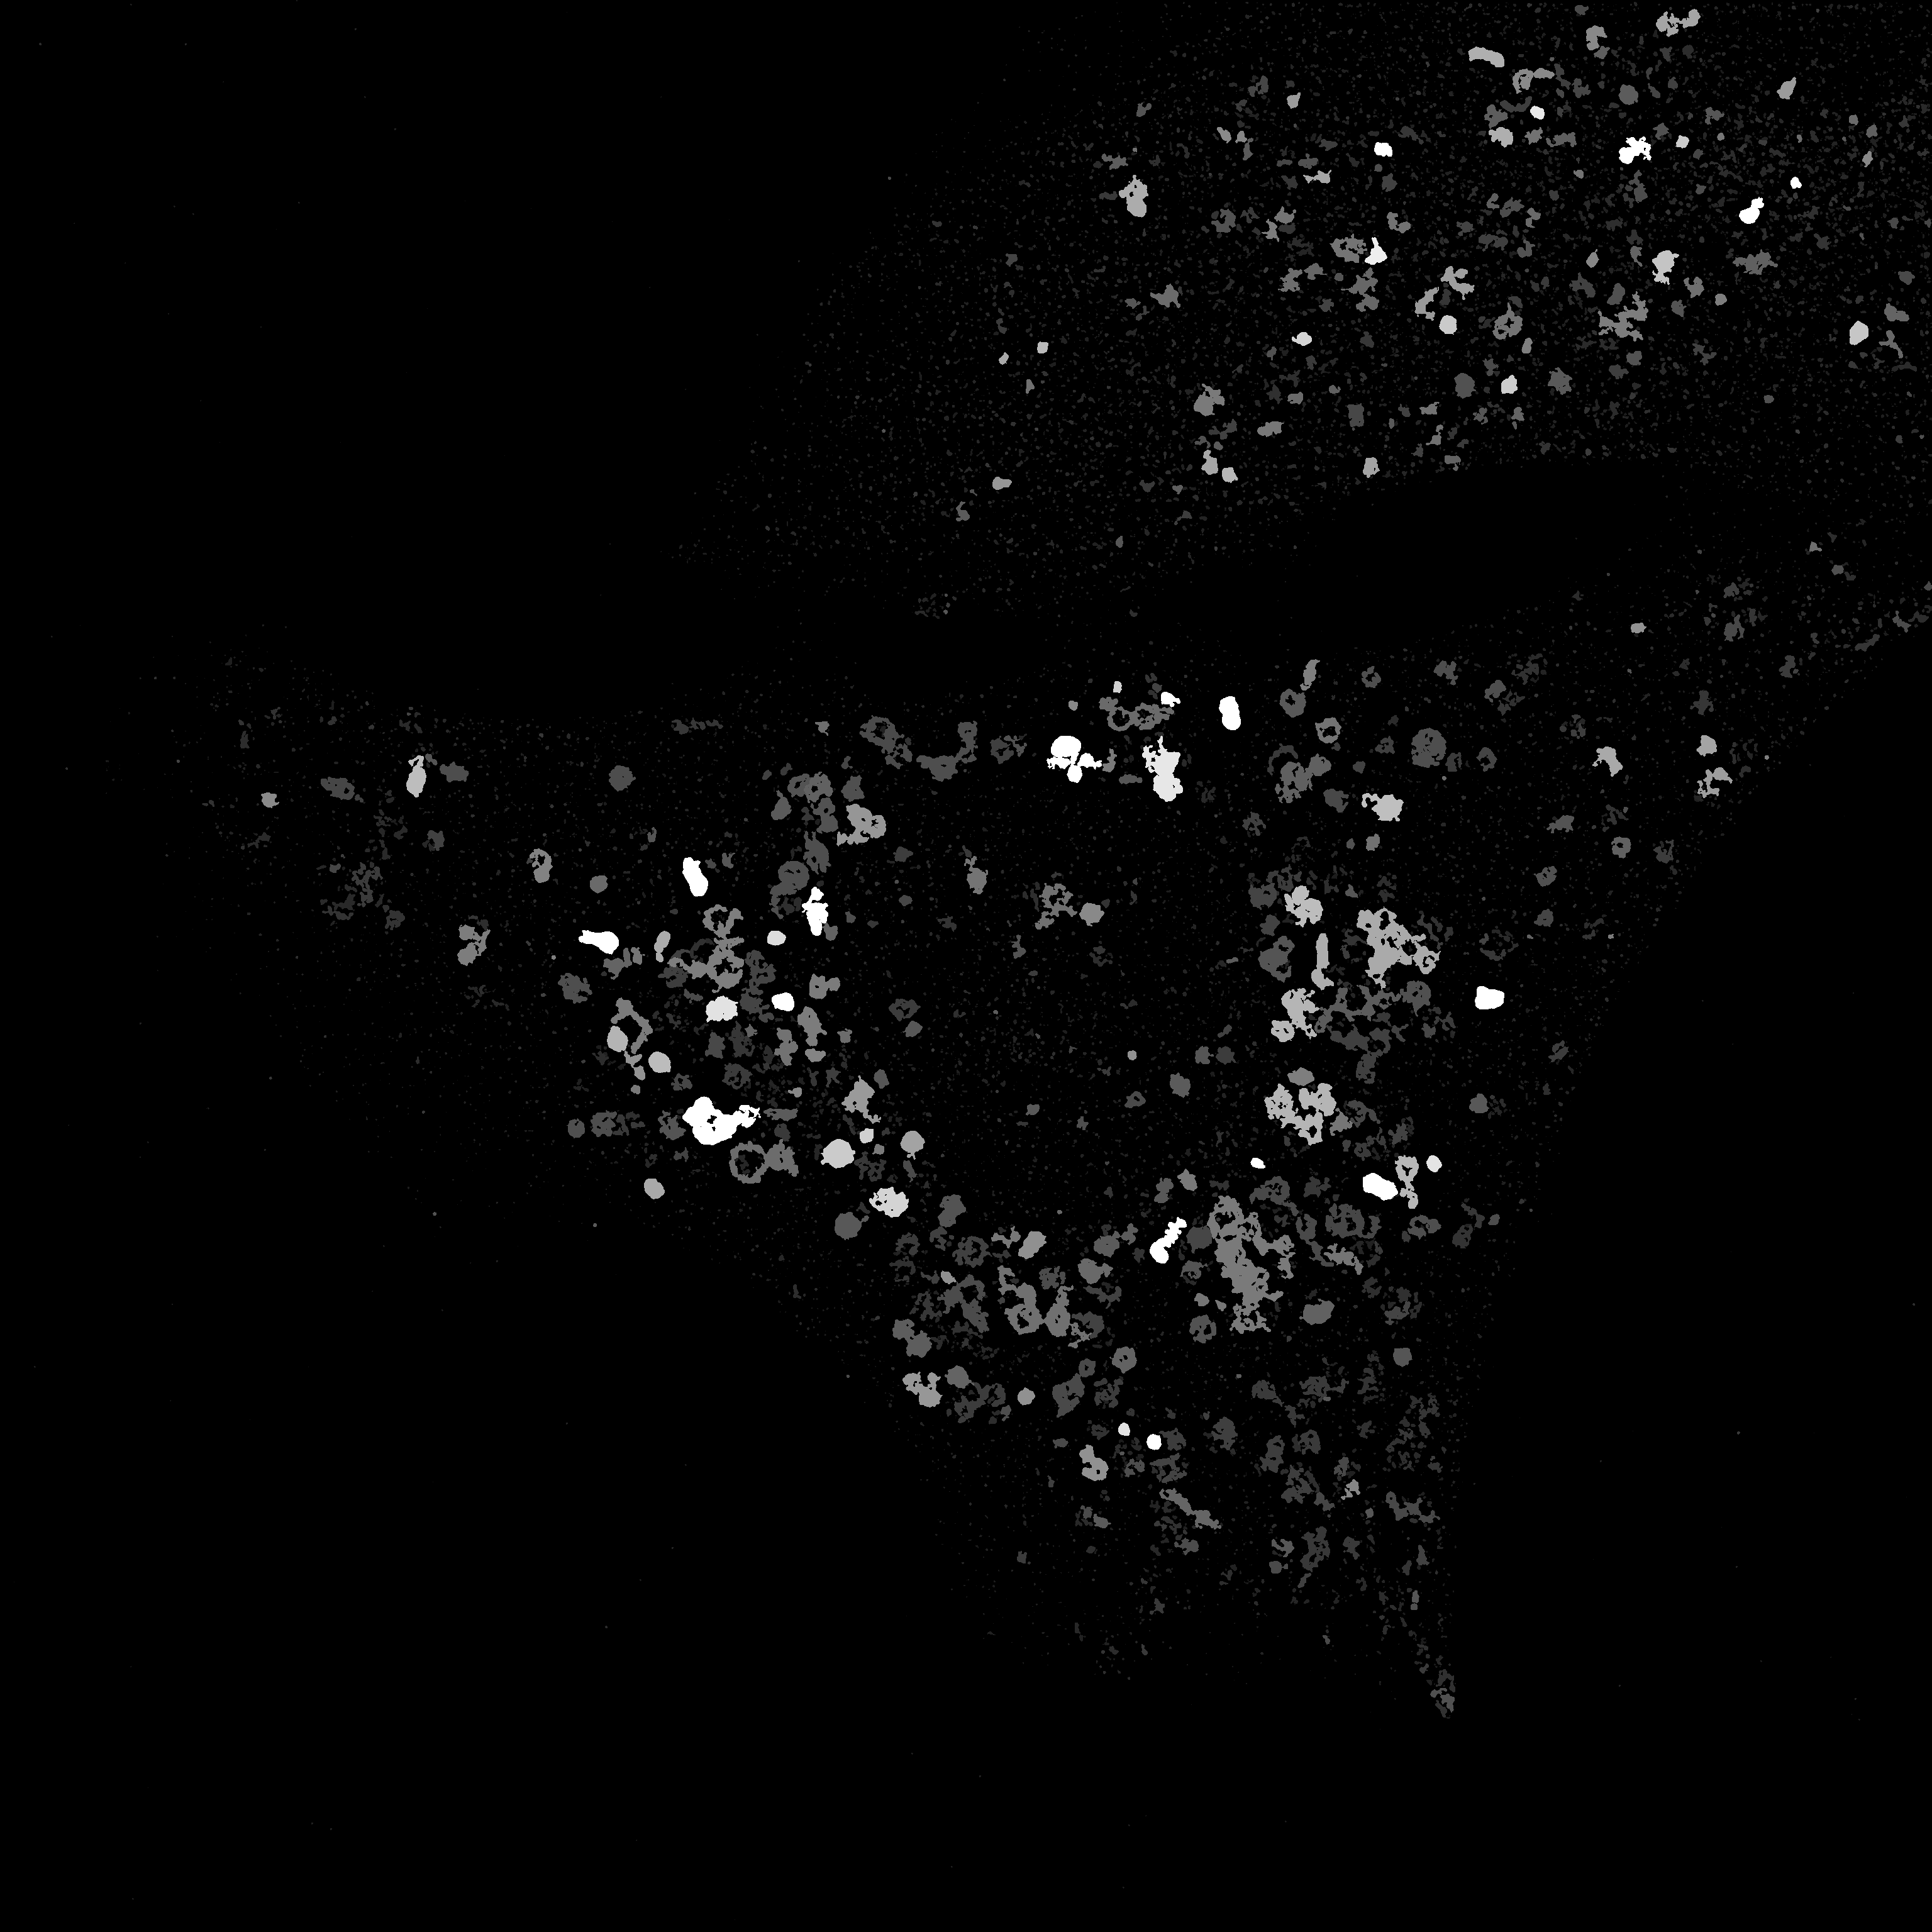
\includegraphics[width=0.49\textwidth]{figs/ch3figs/raw_highlight.png}}
    \subcaptionbox{The high threshold using no window weighting has been applied\label{subfig:window_weight_b}}{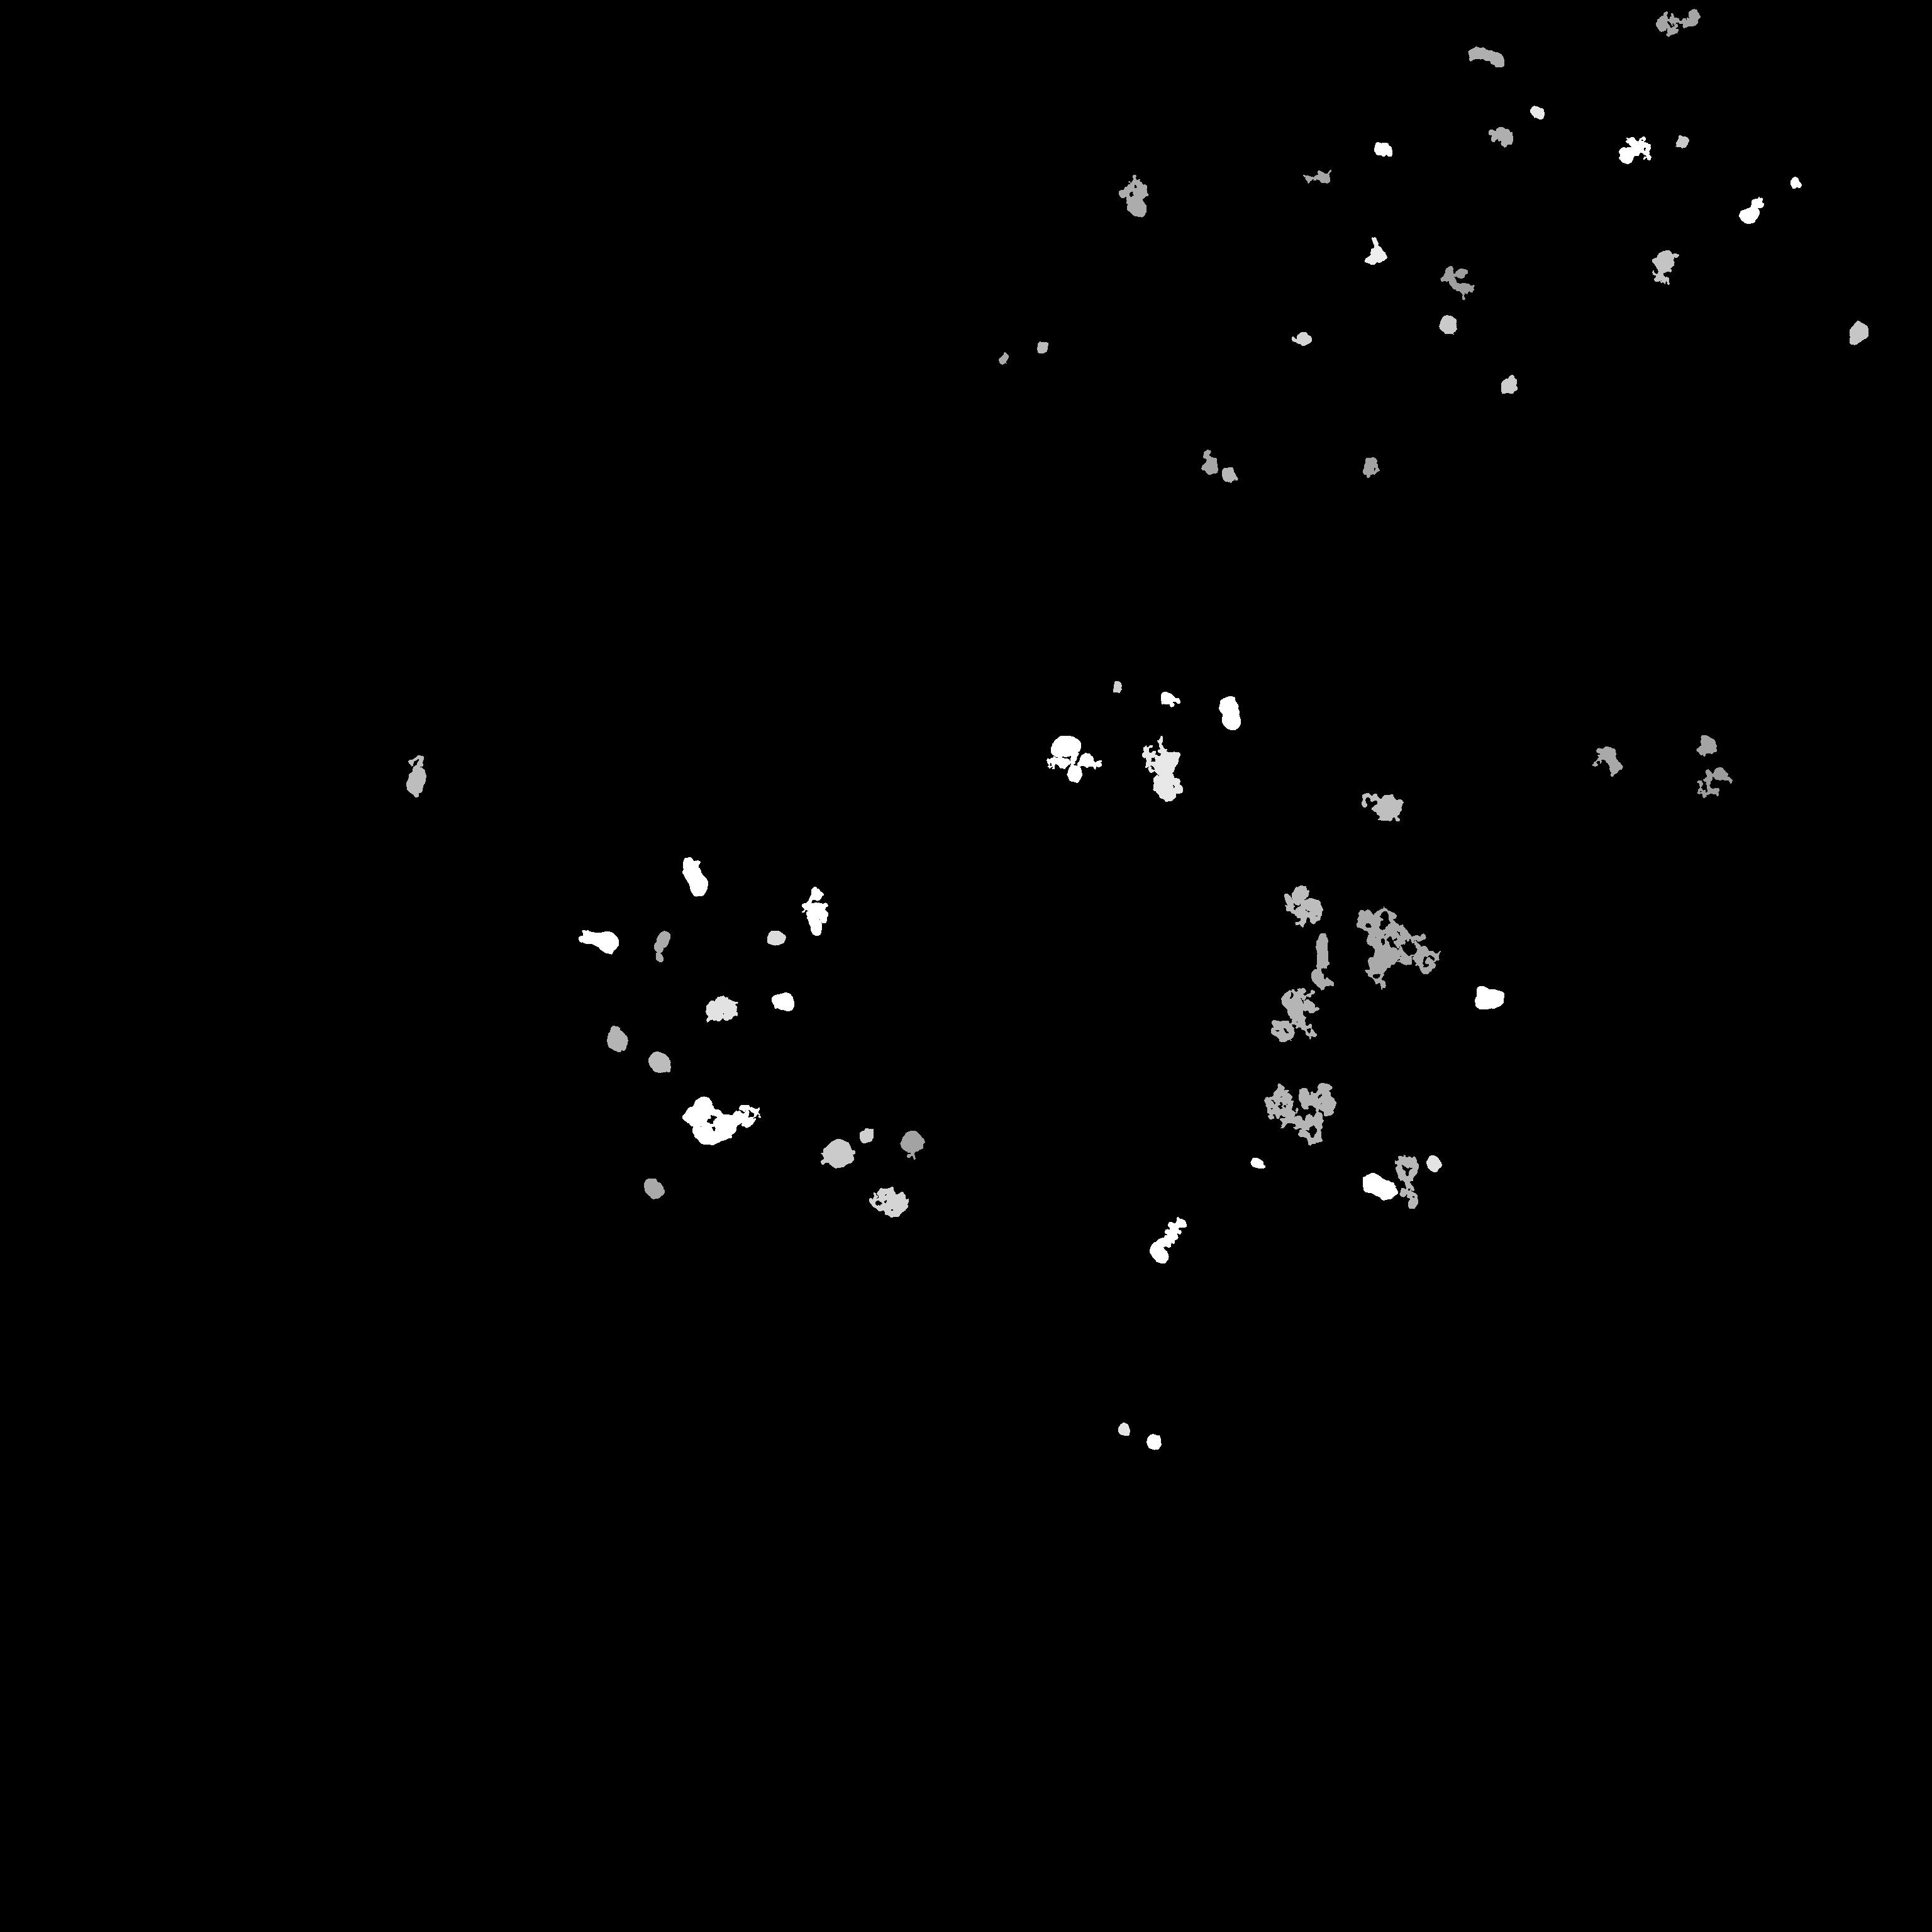
\includegraphics[width=0.49\textwidth]{figs/ch3figs/zero_window.png}}
    \subcaptionbox{The high threshold using the window width weighting has been applied\label{subfig:window_weight_c}}{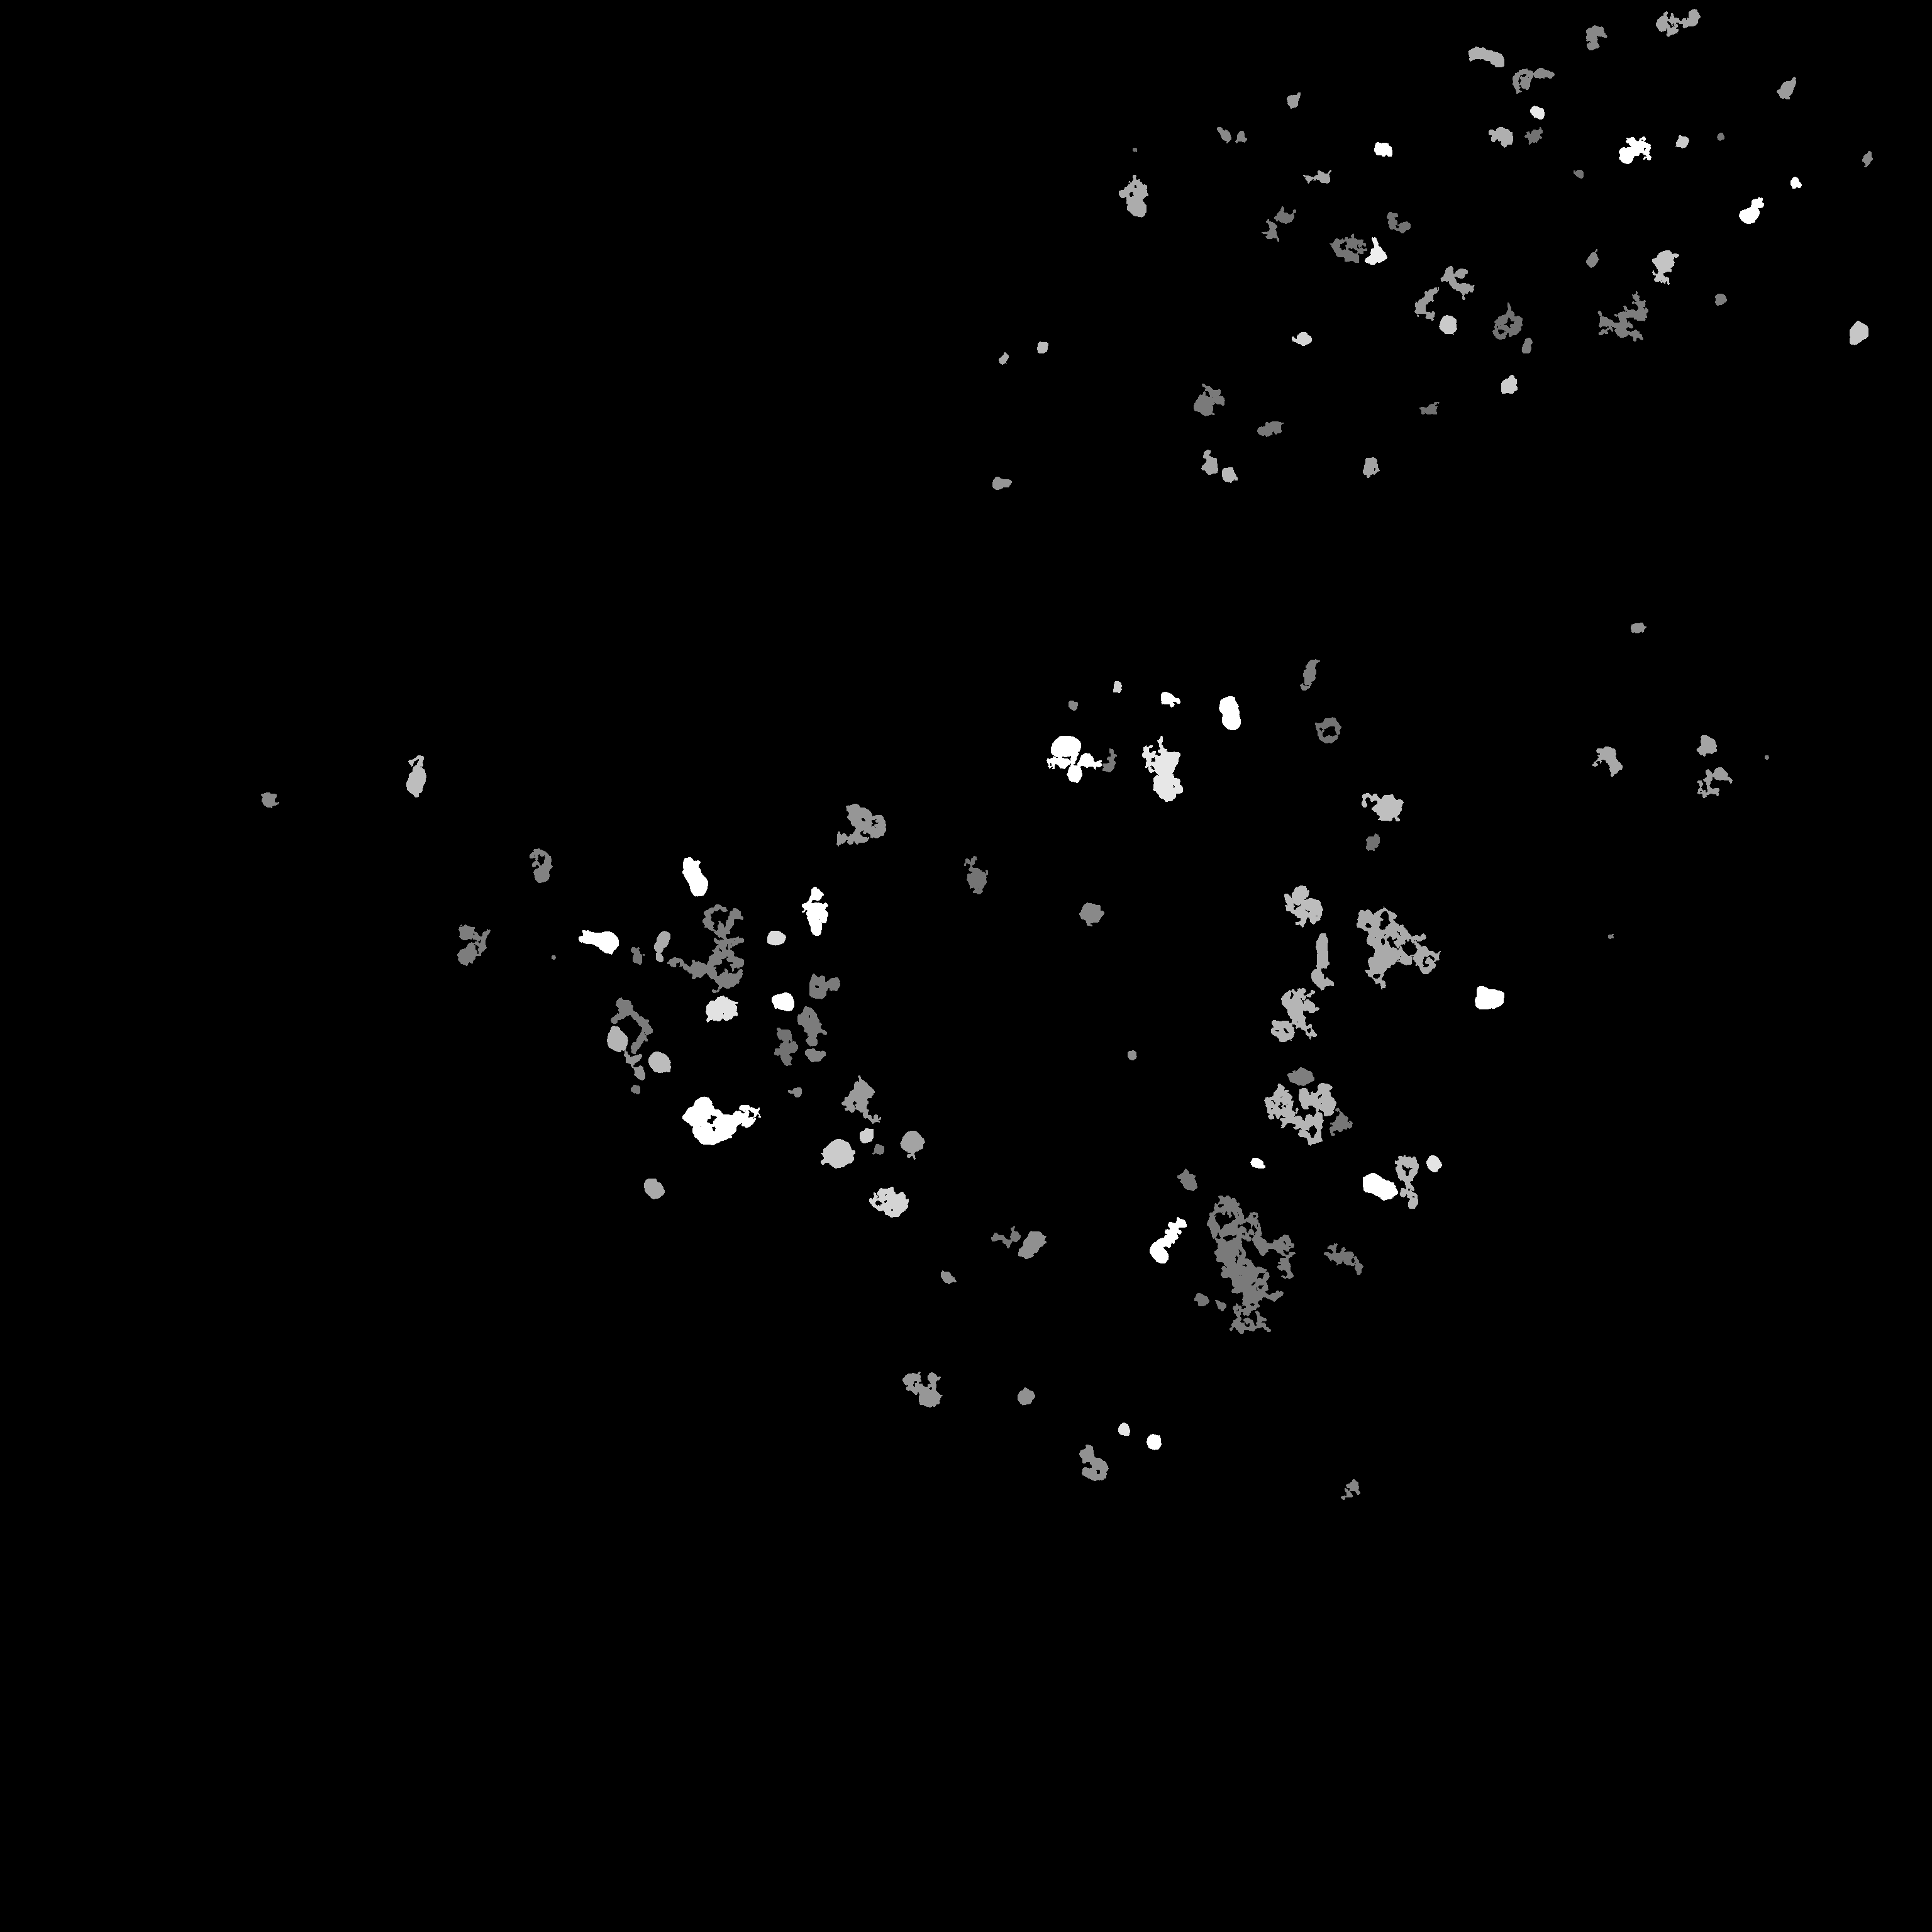
\includegraphics[width=0.49\textwidth]{figs/ch3figs/window_width.png}}
    \subcaptionbox{The high threshold using the window mass weighting has been applied\label{subfig:window_weight_d}}{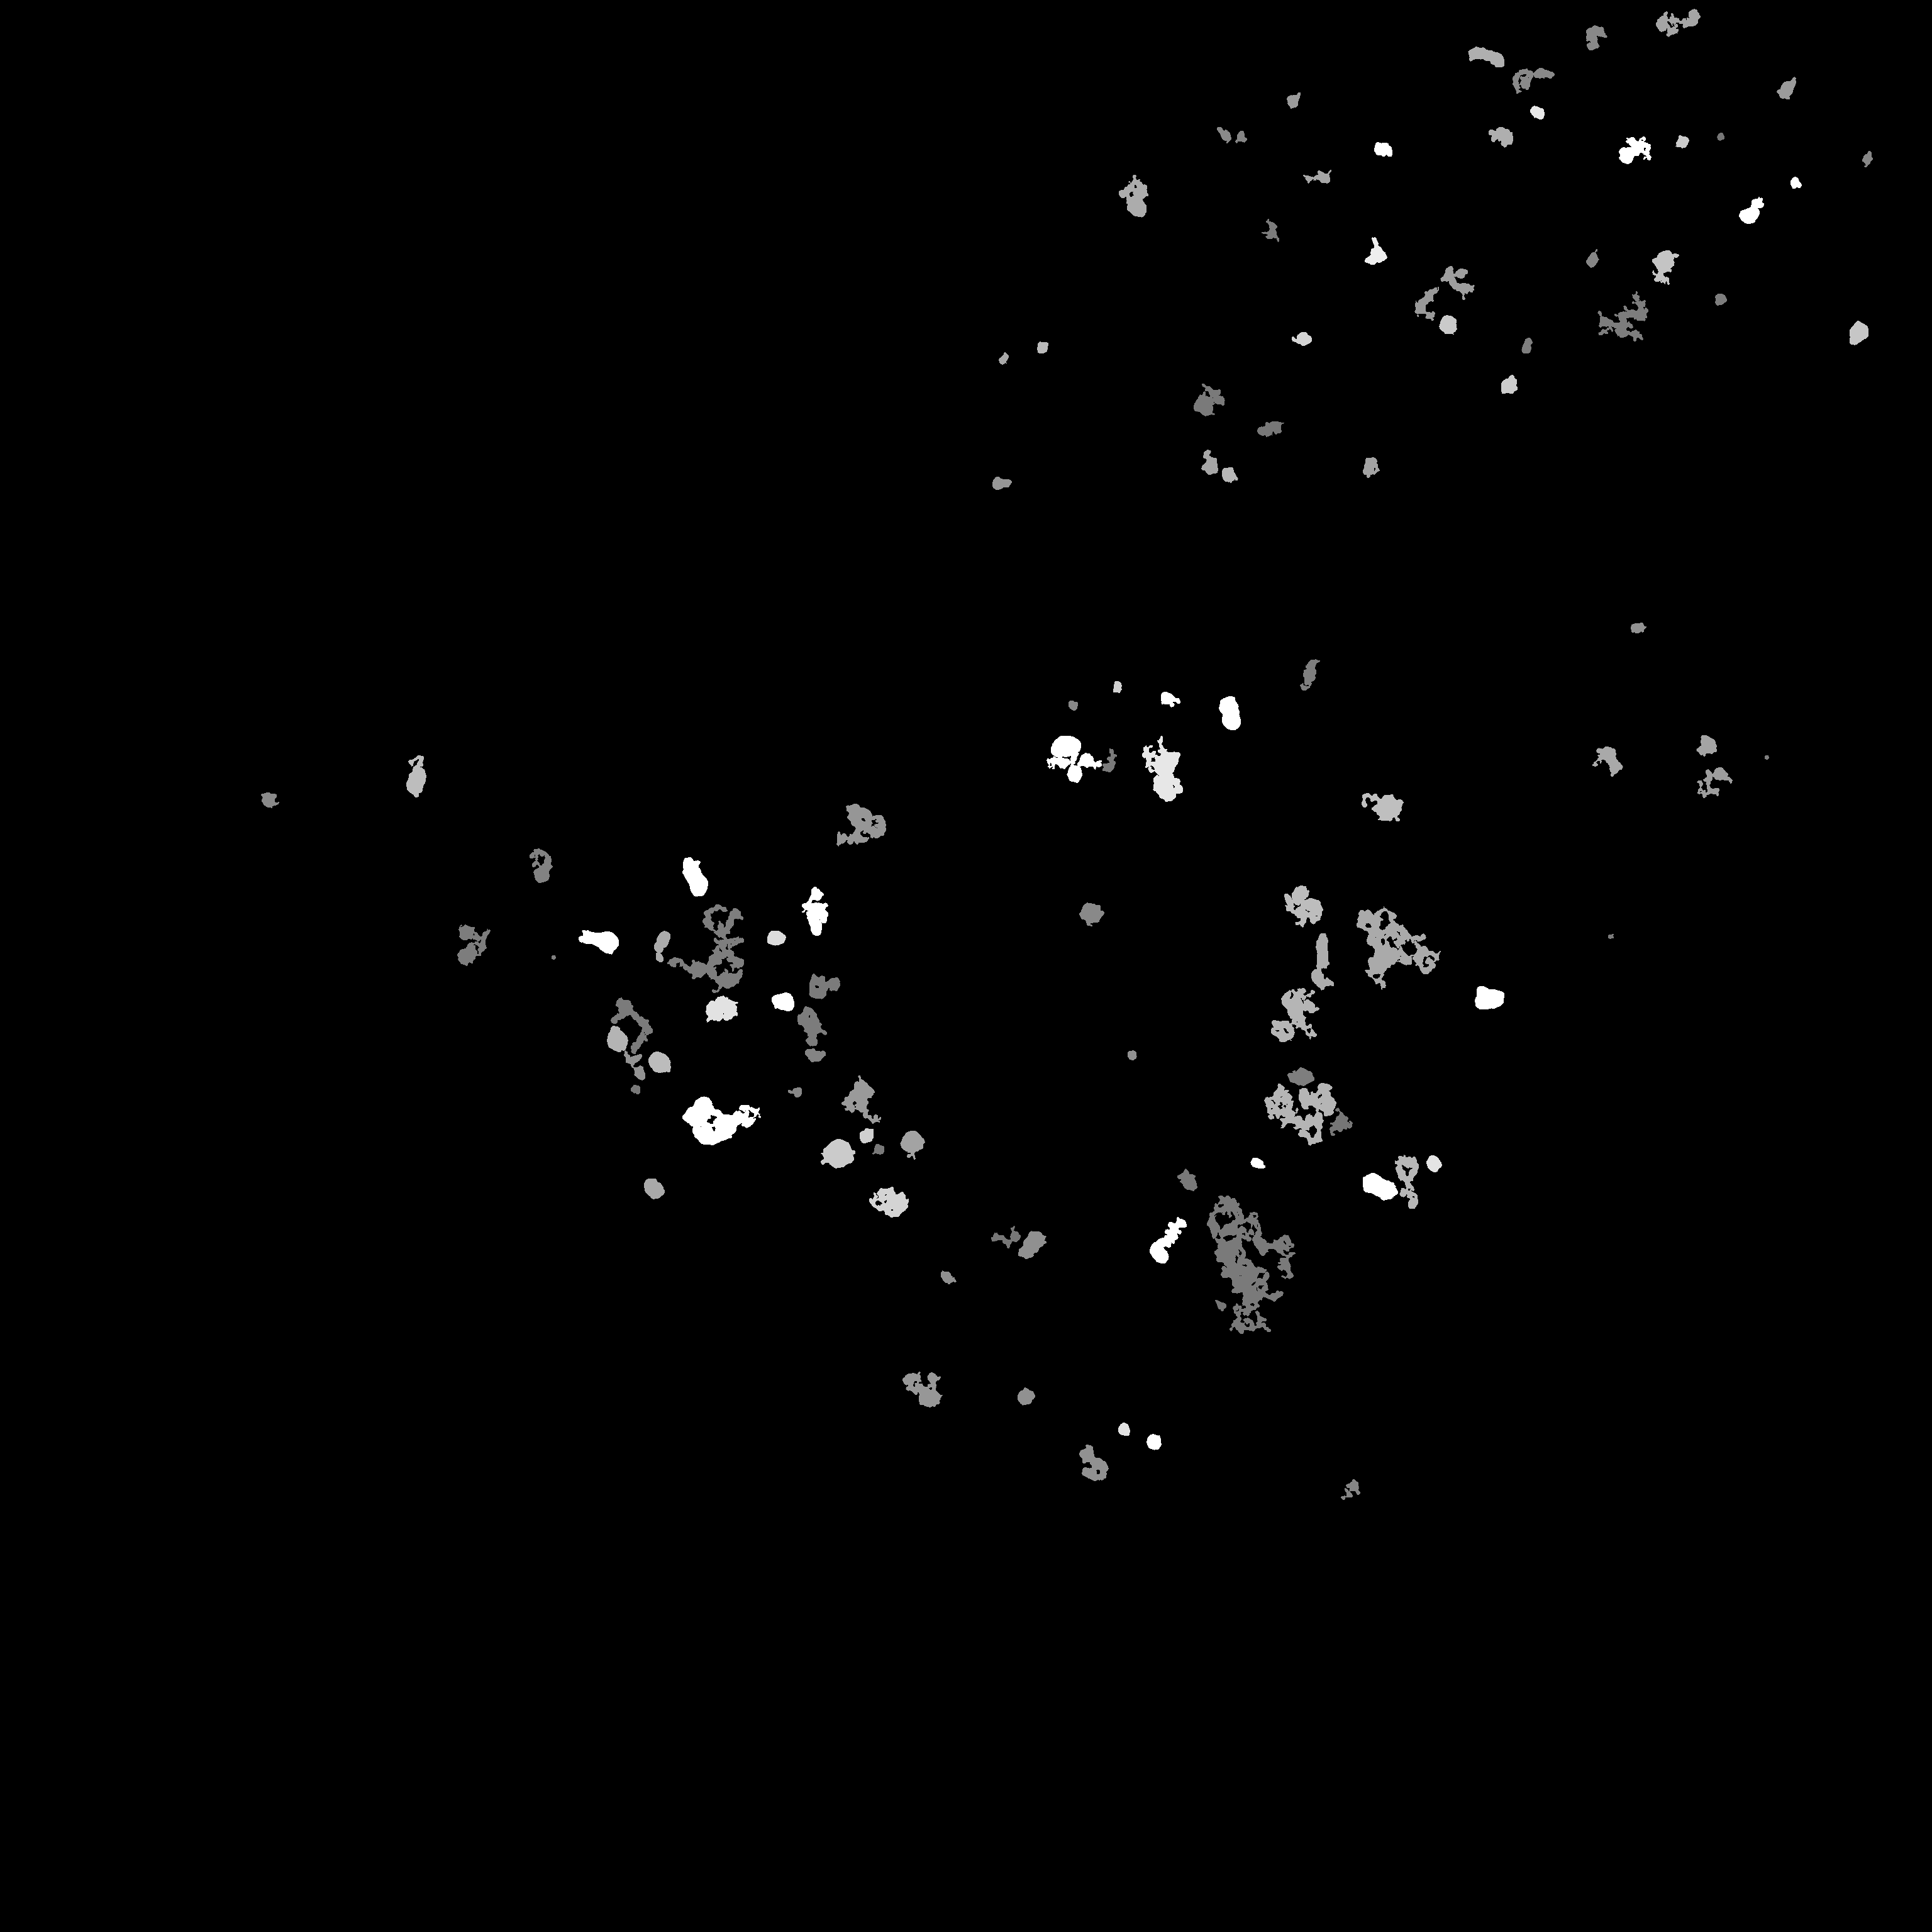
\includegraphics[width=0.49\textwidth]{figs/ch3figs/window_mass.png}}
    \caption[This showcase shows the impact of the window weighting approaches on the determined centroids to be used for the high threshold]{This showcase shows the impact of the window weighting approaches on the determined centroids to be used for the high threshold. The structures shown are highlighted with a brightness proportional to the brightest voxel contained within and are flattened to a 2D MIP image from a 3D image. The original image with only the low threshold applied is shown in (\subref{subfig:window_weight_a}) with high threshold applications shown in (\subref{subfig:window_weight_b}), (\subref{subfig:window_weight_c}), and (\subref{subfig:window_weight_d}). No centroid window weighting biases are applied in (\subref{subfig:window_weight_b}) with a high threshold of $155$ being derived; the window width weighting bias is applied in (\subref{subfig:window_weight_c}) with a high threshold of $112$ being derived; and the window mass weighting bias is applied in (\subref{subfig:window_weight_d}) with a high threshold of $117$}
    \label{fig:window_mips}
\end{figure}

\subsubsection*{Weighting bias summary}
From the exploration of both the IHH weighting bias and the windowing weighting bias approaches detailed thus far it has been observed that the impact the IHH weighting has on the final distribution shape (when combined) can greatly change the final result acquired. The window weighting bias increases the sensitivity to the distribution shape of the lower intensities of the distribution as the shrinking iterating window creates an emphasis on the distribution shape that is maximal at the lowest distribution intensity and diminishes as the intensity increases. Whether this diminishment is linear or non-linear depends on whether the \textbf{window width} weighting or \textbf{window mass} weighting approaches are used respectively. A showcase of this can be seen in Table \ref{tab:window_weighting} where the centroids to be used as the high thresholds for three random sample images are shown. In this table, the centroid values derived without any window weighting, with the window width weighting, and with the window mass weightings are displayed including the added involvement of the IHH bias.
%\rowcolors{2}{yellow!80!red!50}{red!60!yellow!40}
\begin{table}
    \centering
    \begin{tabular}{|c|c|m{0.15\textwidth}|m{0.16\textwidth}|m{0.15\textwidth}|} \hline 
         \textbf{Sample}&  \textbf{IHH Bias}&  \textbf{No Window Weighting}&  \textbf{Window Width Weighting}& \textbf{Window Mass Weighting}\\ \hline 
         A&  False&  155&  112& 117\\ \hline 
         &  True&  107&  87& 85\\ \hline 
         B&  False&  126&  95& 93\\ \hline 
         &  True&  105&  89& 87\\ \hline 
         C&  False&  137&  101& 101\\ \hline 
         &  True&  125&  97& 96\\ \hline
    \end{tabular}
    \caption[Table depicting the effect of the different window weighting approaches on the centroid value for a limited subset of three samples]{The different results of the weighting approaches (no window weighting, window width weighting, window mass weighting) on the final centroid result after consolidation for three random samples is shown. The effect of the IHH bias on the centroid outcome is included as it can have a drastic influence on the behaviour of the window weighting approaches}
    \label{tab:window_weighting}
\end{table}
From the results shown it is observed that the biggest difference is the application of no window weighting versus some window weighting (as mentioned previously), as well as the difference between the two window weighting, approaches not being terribly different although depending on the image, it may only be a single digit shift in value to determine if a structure is labelled as foreground. The biggest difference noted is when the IHH bias is applied but it is speculated that this is due to the IHH distribution being a non-increasing function and thus it is more likely that a greater proportion of the distribution is larger towards the lower intensities and the more aggressive this is the greater the impact the application has on the final centroid result. The expectation is that flatter IHH distributions will have a lesser impact on the centroid results while steeper (or more heavily decreasing distributions) will have a greater impact. This results in a redistribution of the "mass" of the distribution and can lead to low-intensity heavy windows impacting window mass weighting more so than window width weighting.

\section*{Chapter Conclusions}
This chapter has detailed both the methodology behind the preparation of the data used in the development (and testing) of AHT, and the inner workings of the AHT itself. \paragraph{Dataset preparation} is discussed with a focus on the sample preparation prior to microscopy imaging, the microscopy imaging conditions (microscope model, configurations, etc.), and the preprocessing involved with the sample images prior to thresholding which AHT performs.\paragraph{System design} is detailed as the journey to select the thresholding method and motivations behind it, which was Hysteresis thresholding, and how the parameters for said method are to be approximated without any external human involvement. The parameter approximation was the primary focus with the low threshold and high threshold calculation being the two main components. The low threshold determination was the simpler component of the two as multiple methods were compared (including the Kneedle algorithm) with final method being chosen based on quantitative measures and qualitative evaluations of the behaviour of said methods.\par The high threshold was more involved with a novel application of Hysteresis thresholding applied to generate a new distribution from which to analyze the thresholding response of the image in terms of the sensitivity of the total volume of structures to the high threshold selection. Finally, two types of dynamic biasing methods are explored which can tune the high threshold results in a manner that is adaptive to the unique sample image. With the fundamental inner workings of AHT described the proceeding chapters will concern the performance of the AHT relative to other established methods, observations regarding the conditions favourable to AHT, and ending with a conclusion consolidating all of the findings and where that places this research with regard to future interest.